\documentclass{article}

\usepackage{amsmath}
\usepackage{amssymb}
\usepackage{enumerate}
\usepackage[spanish]{babel}
\usepackage{cancel}
\usepackage{caption}
\usepackage[margin=1.5in]{geometry}
\usepackage{graphicx}
\usepackage[utf8]{inputenc}
\usepackage{tcolorbox}
\usepackage{esint}

\renewcommand{\Bbb}{\mathbb}

\tcbuselibrary{theorems}

\begin{document} 

\definecolor{ududff}{rgb}{0.30196078431372547,0.30196078431372547,1}
\definecolor{cqcqcq}{rgb}{0.7529411764705882,0.7529411764705882,0.7529411764705882}

\section{T1}

\subsection{El espacio vectorial $\Bbb R^n$}

El objetivo de la materia es adaptar los conceptos de Análisis I (derivadas, integrales, Taylor ...) al espacio n-dimensional, $\mathbb{R}^n$.

\begin{equation}
x \in \Bbb R^n \Longleftrightarrow x = (x_1, x_2, x_3, ..., x_n)
\end{equation}

Se dice que $x$ es un vector o punto de $\Bbb R^n$, compuesto por $n$ números reales. No se distingue entre vector y punto, salvo que sea necesario.

$\Bbb R^n$ se estructura en espacio vectorial definiendo las siguientes operaciones:

\begin{subequations}
\begin{align}
\forall x, y \in \Bbb R^n, & z = x + y \Longleftrightarrow z_i = x_i + y_i, \forall i \in [1, n] & \text{SUMA VECTORIAL}\\
\forall \alpha \in \Bbb R, & x \in \Bbb R^n, z = \alpha x \Longleftrightarrow z_i = \alpha x_i \forall i \in [1, n] & \text{PRODUCTO POR ESCALAR}
\end{align}
\end{subequations}

Con estas definiciones, puede probarse que $\Bbb R^n$ es cerrado para la suma vectorial y producto por un escalar, considerando el vector nulo (todos ceros), $\overline{0}$, como el neutro para la suma, y el número real 1 como el neutro del producto por escalar.

Adicionalmente, $\Bbb R^n$ pasa a ser un \textbf{espacio vectorial euclídeo} si se le agrega un \textbf{producto escalar}:

\begin{equation}
\forall x, y \in \Bbb R^n, \alpha = x \cdot y \Longleftrightarrow \alpha = \sum\limits_{i=1}^{n} x_i y_i = x_1 y_1 + x_2 y_2 + ... + x_n y_n
\end{equation}

Definiendo una \textbf{norma} sobre el producto escalar, $\Bbb R^n$ pasa a ser un espacio vectorial euclídeo y normado. La norma canónica en $\Bbb R^n$ es la raíz cuadrada del producto escalar del vector consigo mismo:

\begin{equation}
\forall x \in \Bbb R^n, \|x\| = \sqrt{x \cdot x} = \sqrt{ \sum\limits_{i=1}^{n} x_i^2 }
\end{equation}

Un \textbf{versor} es un vector de norma 1. Para "normalizar" cualquier vector, se lo divide por su norma:

\begin{equation}
\forall x \in \Bbb R^n, \left\| \frac{x}{\|x\|} \right\| = 1
\end{equation}

\subsection{Ángulo entre dos vectores - Proyección}

Si $x, y \neq \overline{0}$, el ángulo entre x e y, $\alpha(x,y)$, satisface la siguiente igualdad:

\begin{equation}
\cos (\alpha(x, y)) = \frac{x \cdot y}{ \|x\| \|y\| }
\end{equation}

\begin{figure}[t]
\caption{Proyección del vector x sobre el vector y}
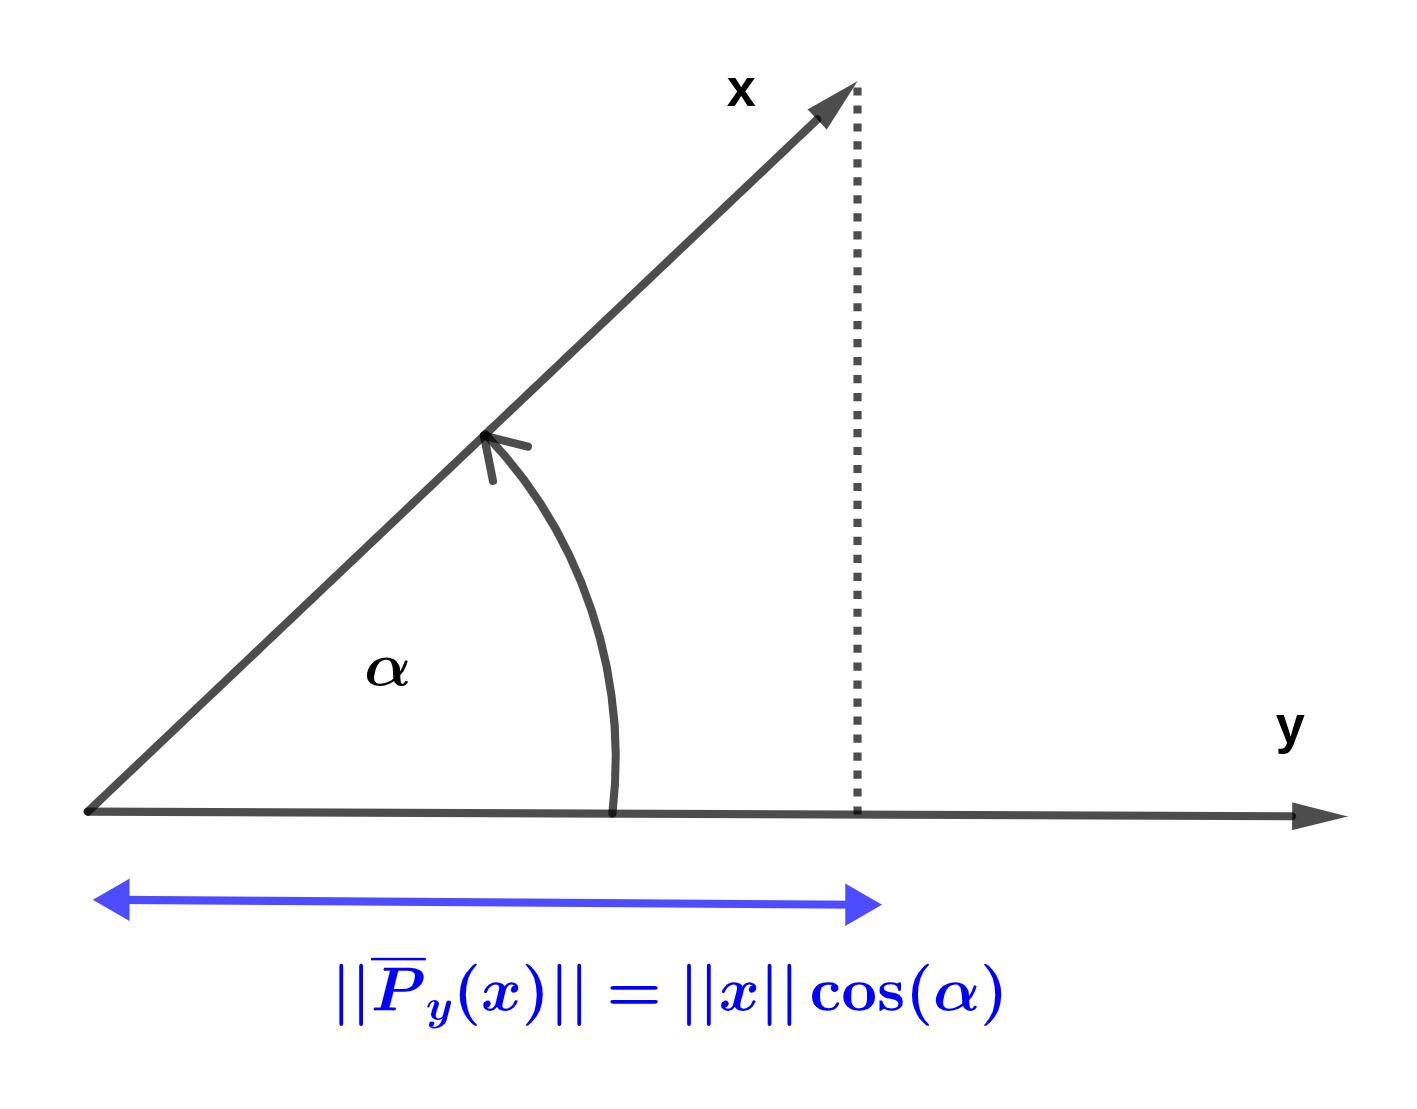
\includegraphics[scale=1]{img/teo_fig001_proyeccion.png} 
\centering
\label{fig:proyeccion}
\end{figure}

Aplicando la igualdad del ángulo entre vectores, y considerando el versor $\breve{y} = \frac{y}{\|y\|}$, resulta:

\begin{equation}
x \cdot y = \|x\| \|y\| \cos(\alpha) \Longrightarrow x \cdot \breve{y} = \|x\| \underbrace{ \cancel{ \| \breve{y} \| } }_{\text{Norma 1}} \cos(\alpha) = \|x\| \cos(\alpha)
\end{equation}

Geométricamente, como se observa en la figura ~\ref{fig:proyeccion}, la proyección de x sobre y se obtiene como el siguiente vector:

\begin{equation}
\overline{P}_{y}(x) =  \underbrace{ \|x\| \cos(\alpha) }_{\text{Escalar}}  \underbrace{ \breve{y} }_{\text{Versor}}
\end{equation}

\begin{equation}
\tcboxmath[colback=orange!25!white,colframe=orange, title=Proyección de x sobre y]
{ \overline{P}_{y}(x) = (x \cdot \breve{y}) \breve{y} }
\end{equation}

\begin{subequations}
\begin{align}
\overline{P}_{y}(x) = \overline{0} & \Longleftrightarrow x \perp y \Longleftrightarrow \cos \alpha = 0 \\
\overline{P}_{y}(x) = x & \Longleftrightarrow x = \alpha y, \alpha > 0
\end{align}
\end{subequations}

\subsection{Distancia entre dos puntos}

$\forall x, y \in \Bbb R^n$, se define la distancia entre x e y como:

\begin{equation}
d(x,y) = \| x - y \| = \| y - x \|
\end{equation}

\subsection{Producto vectorial}

Sólo para $\Bbb R^3$, se define el \textbf{producto vectorial} como:

\begin{equation}
\forall x, y \in \Bbb R^3: x \otimes y = \begin{vmatrix}
    \breve{i} & \breve{j} & \breve{k} \\
    x_1 & x_2 & x_3 \\ 
    y_1 & y_2 & y_3
  \end{vmatrix} =
\left(
  \begin{vmatrix} x_2 & x_3 \\ y_2 & y_3 \end{vmatrix},
  -\begin{vmatrix} x_1 & x_3 \\ y_1 & y_3 \end{vmatrix},
  \begin{vmatrix} x_1 & x_2 \\ y_1 & y_2 \end{vmatrix}
\right)
\end{equation}

Propiedades:

\begin{subequations}
\begin{align}
x \otimes y & \perp x \\
x \otimes y & \perp y \\
x \otimes y & = -y \otimes x \\
\| x \otimes y \| & = \|x\| \|y\| \sin(\alpha(x,y)) = \text{Área del paralelogramo determinado por x e y} \\
x \otimes y & = \overline{0} \Longleftrightarrow \{x, y\} \text{ es linealmente dependiente} \Longleftrightarrow x \parallel y
\end{align}
\end{subequations}

\subsection{Clasificación de puntos en un subconjunto de $\Bbb R^n$}

Sea un punto $P_0 \in \Bbb R^n$; se define como \textbf{bola o entorno} de centro $P_0$ y radio $r$ al conjunto de puntos cuya distancia a $P_0$ es menor que $r$. Simbólicamente:

\begin{equation}
B(P_0, r) = \{ x \in \Bbb R^n / \| x - P_0 \| < r \}
\end{equation}

En $\Bbb R$, esto es un intervalo abierto; en $\Bbb R^2$, el interior de un círculo; en $\Bbb R^3$, el interior de una esfera. Para dimensiones mayores, no hay tal representación geométrica, pero la definición se mantiene.

Si se excluye al centro $P_0$, se habla de una bola o entorno \textbf{reducido}:

\begin{equation}
B^*(P_0, r) = B(P_0, r) - \{ P_0 \}
\end{equation}

Considérese a continuación un subconjunto $A \subseteq \Bbb R^n$

\subsubsection{Punto interior}

$P_0$ es punto interior de $A \Longleftrightarrow \exists B(P_0, r) \subset A$. Es decir, si existe al menos un entorno centrado en $P_0$ que esté incluido en $A$. En otras palabras, $P_0$ está "rodeado por todas partes" de puntos de $A$.

Por otro lado, se define al \textbf{conjunto interior de} $A$, notado $\mathring{A}$, de la siguiente manera:

\begin{equation}
\mathring{A} = \{ x \in \Bbb R^n / x \text{ es punto interior de } A \}
\end{equation}

\subsubsection{Punto exterior}

$P_0$ es punto exterior de $A \Longleftrightarrow \exists B(P_0, r) \subset A^c$. Es decir, un punto es exterior de $A$ si es interior del complemento de $A$ ($A^c$).

\begin{equation}
Ext(A) = \{ x \in \Bbb R^n / x \text{ es p.e. de A } \}
\end{equation}

\subsubsection{Punto frontera}

$P_0$ es punto frontera de $A \Longleftrightarrow$ toda bola centrada en $P_0$ contiene elementos de $A$ y $A^c$. Simbólicamente:

\begin{equation}
P_0 \text{ es p.f. de } A \Longleftrightarrow \forall B(P_0, r), \left\{
\begin{array}{ll}
B(P_0, r) \cap A \neq \varnothing \\
B(P_0, r) \cap A^c \neq \varnothing
\end{array}
\right.
\end{equation}

La \textbf{frontera} de $A$, $\partial A$, se define como:

\begin{equation}
\partial A = \{ x \in \Bbb R^n / x \text{ es p.f. de A } \}
\end{equation}

Propiedades:

\begin{subequations}
\begin{align}
\mathring{A} \cap \partial A & = \varnothing \\
Ext(A) \cap \partial A & = \varnothing \\
\mathring{A} \cap Ext(A) & = \varnothing \\
\mathring{A} \cup \partial A \cup Ext(A) & = \Bbb R^n \\
\text{Clausura/adherencia de A } = \overline{A} & = A \cup \partial A \\
\text{A es abierto } \Longleftrightarrow A & = \mathring{A} \\
\text{A es cerrado } \Longleftrightarrow A & = \overline{A} \Longleftrightarrow A^c \text{ es abierto } \\
\end{align}
\end{subequations}

\subsubsection{Punto aislado}

$P_0$ es p.a. $\Longleftrightarrow \exists B^*(P_0, r) / B^*(P_0, r) \cap A = \varnothing$.

O sea, hay al menos un entorno reducido centrado en $P_0$ que no contiene otro elemento de $A$ aparte de $P_0$.

\subsubsection{Punto de acumulación}

$P_0$ es p. de ac. $\Longleftrightarrow \forall B^*(P_0, r), B^*(P_0, r) \cap A \neq \varnothing$.
Vale decir, en todo entorno reducido de $P_0$ hay elementos de $A$. El conjunto derivado de $A$, denotado $A'$, se define como el conjunto de todos los puntos de acumulación de $A: A' = \{ x \in \Bbb R^n / x \text{ x es p. de ac. de A} \}$

\subsection{Cónicas}

Las cónicas son curvas planas (bidimensionales) que se obtienen al seccionar un cono (tridimensional) de diferentes maneras.

\subsubsection{Circunferencia}

\begin{equation}
(x-x_0)^2 + (y-y_0)^2 = r^2, \text{ siendo r el radio y } (x_0, y_0) \text{ el centro}
\end{equation}

\subsubsection{Elipse}

\begin{equation}
\frac{(x-x_0)^2}{a^2} + \frac{(y-y_0)^2}{b^2} = 1, \text{ siendo a el semieje x, b el semieje y, y } (x_0, y_0) \text{ el centro}
\end{equation}

\subsubsection{Parábolas}

Parábola vertical:

\begin{equation}
y = a (x-c)^2 + b
\end{equation}

Parábola horizontal:

\begin{equation}
x = a (y-c)^2 + b
\end{equation}

\subsubsection{Hipérbolas}

\begin{equation}
\frac{(x-x_0)^2}{a^2} - \frac{(y-y_0)^2}{b^2} = 1
\end{equation}

\begin{figure}[t]
\caption{Hipérbolas}
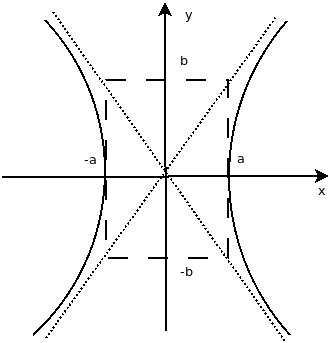
\includegraphics[scale=0.8]{img/pra_fig001_hiperbolas.png} 
\centering
\label{fig:hiperbolas}
\end{figure}

En la hipérbola de la figura ~\ref{fig:hiperbolas}, $a$ es el semilado $x$ del rectángulo, y $b$ corresponde al semilado $y$. El centro del rectángulo es el punto $(x_0, y_0)$, que en el dibujo corresponde al origen. 
Nótese además que las diagonales del rectángulo definido por $a$ y $b$ son asíntotas oblicuas de la cónica. Por otro lado, el eje que la curva no corta es el asociado al término negativo ($y$ en este ejemplo).

\subsection{Planos}

La \textbf{forma implícita} de definir un plano en $\Bbb R^3$ es:

\begin{equation}
\overline{N} \cdot (\overline{Q} - \overline{P}) = 0
\end{equation}

En este esquema, $P$ y $Q$ son dos puntos pertenecientes al plano, y $N$ es la \textbf{normal}, un vector ortogonal al plano.

Por otro lado, se tiene la \textbf{forma vectorial}:

\begin{equation}
(x,y,z) = \alpha (p_1, p_2, p_3) + \beta (q_1, q_2, q_3) + R
\end{equation}

En esta forma, $P = (p_1, p_2, p_3)$ y $Q = (q_1, q_2, q_3)$ son dos vectores, no puntos; es importante la distinción en este caso; pensar a los vectores como segmentos orientados para distinguirlos de los puntos. De ese modo, $P$ y $Q$ son vectores contenidos en el plano, en tanto $R$ es un punto contenido en el mismo. Los parámetros $\alpha$ y $\beta$ son reales, y sus combinaciones de valores cubren todo el plano definido. 

\section{T2 - Funciones}

\begin{subequations}
\begin{align}
&f: A \rightarrow B \\
&A = \text{dominio de f} \\
&B = \text{codominio/imagen de f} = Im(f) \\
&\text{Gráfico de f } = G(f) = \{ (x, f(x)) \text{ con x } \in A \}
\end{align}
\end{subequations}

Si $A \subset \Bbb R^n$ y $B \subset \Bbb R^m$, entonces $G(f) \subset \Bbb R^(n+m)$.

$x$ es el argumento de $f$, y $f(x)$ es la imagen de $x$ a través de $f$.

\subsection{Preimagen}

\begin{equation}
f^{-1}(H) = \{ x \in A / f(x) \in H \}
\end{equation}

$f^{-1}(H)$ NO es la inversa de $f$; esto es notación.

En palabras, la preimagen del conjunto $H$ consiste de los elementos del dominio cuya imagen a través de $f$ pertenece a $H$.

\begin{equation}
H \cap Im(f) = \varnothing \Longrightarrow f^{-1}(H) = \varnothing
\end{equation}

\subsection{Tipos de funciones}

i) Funciones escalares: $A \subset \Bbb R$, $B \subset \Bbb R \Longrightarrow f: \Bbb R \rightarrow \Bbb R$

ii) Campos escalares: $A \subset \Bbb R^n, B \subset \Bbb R \Longrightarrow \overline{f}: \Bbb R^n \rightarrow \Bbb R$

iii) Funciones vectoriales (curvas): $A \subset \Bbb R, B \subset \Bbb R^n \Longrightarrow \overline{f}: \Bbb R \rightarrow \Bbb R^n$

iv) Campos vectoriales: $A \subset \Bbb R^n, B \subset \Bbb R^m \Longrightarrow \overline{f}: \Bbb R^n \rightarrow \Bbb R^m$

\subsection{Conjuntos de nivel}

Partiendo de la definición de preimagen, si $H$ tiene un único elemento $u$, se llama conjunto de nivel $u$ de $f$ a:

\begin{equation}
C_u(f) = \{ x \in A / f(x) = u, u \in B \}
\end{equation}

$u$ puede ser un vector o escalar.

\subsection{Conjunto conexo}

$A \subset \Bbb R^n$ es conexo $\Longleftrightarrow \nexists \text{ dos conjuntos } A_1 y A_2 / A = A_1 \cup A_2$, con $\overline{A_1} \cap A_2 = \varnothing \wedge A_1 \cap \overline{A_2} = \varnothing$.

O sea, no se puede "partir en dos" a $A$.

Construyendo sobre esta definición, $A \subset \Bbb R^n$ es \underline{arco-conexo} si cualquier par de puntos de $A$ puede ser unido a través de una curva continua. Simbólicamente:

\begin{equation}
A \subset \Bbb R^n \text{ es arco-conexo } \Longleftrightarrow \exists \overline{f}: [a,b] \rightarrow A / \overline{f}(a) = x \wedge \overline{f}(b) = y \forall x,y \in A
\end{equation}

\subsection{Conjunto acotado}

$A \subset \Bbb R^n$ es acotado $\Longleftrightarrow \forall x \in A, \exists M > 0 / \|x\| < M$. Vale decir, todo $A$ puede ser contenido en una bola de radio $M$.

\subsection{Coordenadas polares}

En el sistema de coordenadas cartesianas en $\Bbb R^2$, se miden las proyecciones del vector posición sobre el eje $x$ y el eje $y$. En cambio, en el sistema de coordenadas polares, se miden el ángulo respecto al eje $x$ (coordenada $\phi$), y la distancia desde el origen al punto sobre la recta asociada a dicho ángulo (coordenada $\rho$).

\begin{figure}[t]
\caption{Coordenadas polares}
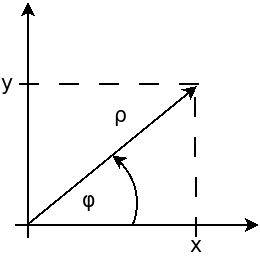
\includegraphics[scale=1.0]{img/pra_fig002_polares.png} 
\centering
\label{fig:polares}
\end{figure}

Conversión de C.C. a C.P.:

\begin{subequations}
\begin{align}
x & = \rho \cos \phi \\
y & = \rho \sin \phi
\end{align}
\end{subequations}

Conversión de C.P. a C.C.:

\begin{subequations}
\begin{align}
\rho & = \sqrt{x^2 + y^2} \\
\phi & = \arctan \left( \frac{y}{x} \right)
\end{align}
\end{subequations}

\subsection{Cuádricas}

Las cuádricas son superficies en $\Bbb R^3$ que encierran un volumen.

\subsubsection{Esfera}

\begin{equation}
(x-x_0)^2 + (y-y_0)^2 + (z-z_0)^2 = r^2
\end{equation}

\subsubsection{Elipsoide}

\begin{equation}
\frac{(x-x_0)^2}{a^2} + \frac{(y-y_0)^2}{b^2} + \frac{(z-z_0)^2}{c^2} = 1
\end{equation}

\subsubsection{Paraboloide}

\begin{equation}
\frac{(x-x_0)^2}{a^2} + \frac{(y-y_0)^2}{b^2} = z
\end{equation}

Con esta definición, el paraboloide se proyecta sobre $z$ (puede ser sobre $x$ o $y$, intercambiando las variables).

\subsubsection{Cilindro}

Circular recto, sobre el eje $z$:

\begin{equation}
(x-x_0)^2 + (y-y_0)^2 = r^2, z \in \Bbb R
\end{equation}

Elíptico recto, sobre el eje $z$:

\begin{equation}
\frac{(x-x_0)^2}{a^2} + \frac{(y-y_0)^2}{b^2} = 1, z \in \Bbb R
\end{equation}

\subsubsection{Cono}

Circular:

\begin{equation}
(x-x_0)^2 + (y-y_0)^2 = (z-z_0)^2
\end{equation}

Elíptico:

\begin{equation}
\frac{(x-x_0)^2}{a^2} + \frac{(y-y_0)^2}{b^2} = (z-z_0)^2
\end{equation}

\subsubsection{Hiperboloide (1 hoja)}

\begin{equation}
\frac{(x-x_0)^2}{a^2} + \frac{(y-y_0)^2}{b^2} - \frac{(z-z_0)^2}{c^2} = 1
\end{equation}

\begin{figure}[t]
\caption{Hiperboloide (1 hoja)}
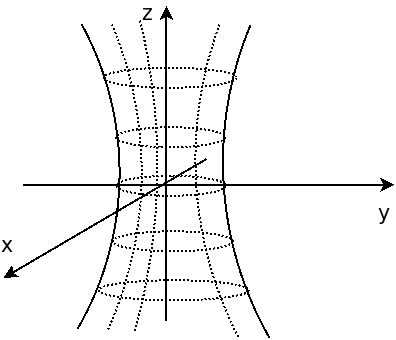
\includegraphics[scale=0.75]{img/pra_fig003_hiperboloide1.png} 
\centering
\label{fig:hiperboloide1}
\end{figure}

\subsubsection{Hiperboloide (2 hojas)}

\begin{equation}
-\frac{(x-x_0)^2}{a^2} - \frac{(y-y_0)^2}{b^2} + \frac{(z-z_0)^2}{c^2} = 1
\end{equation}

\begin{figure}[t]
\caption{Hiperboloide (2 hojas)}
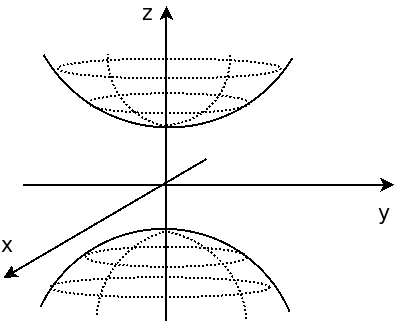
\includegraphics[scale=0.75]{img/pra_fig004_hiperboloide2.png} 
\centering
\label{fig:hiperboloide2}
\end{figure}

\subsubsection{Paraboloide hiperbólico}

\begin{equation}
-\frac{(x-x_0)^2}{a^2} + \frac{(y-y_0)^2}{b^2} = \frac{z-z_0}{c}
\end{equation}

\begin{figure}[t]
\caption{Paraboloide hiperbólico}
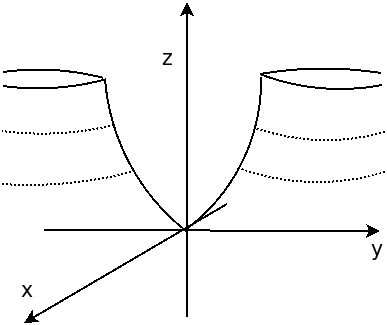
\includegraphics[scale=0.75]{img/pra_fig005_paraboloide_h.png} 
\centering
\label{fig:paraboloide_h}
\end{figure}

\section{T3 - Límite y continuidad}

Un plano puede verse como la imagen de un campo vectorial. Si $\pi: P_0 + \alpha \overrightarrow{u} + \beta \overrightarrow{v}$ (el plano que pasa por $P_0$ y es generado por $\overrightarrow{u}$ y $\overrightarrow{v}$, entonces puede definirse el siguiente campo vectorial:

\begin{equation}
\overline{f}: \Bbb R^2 \rightarrow \Bbb R^3 / \overline{f}(\alpha, \beta) = (x, y, z) = P_0 + \alpha \overrightarrow{u} + \beta \overrightarrow{v}
\end{equation}

Algo análogo puede hacerse con la recta:

\begin{equation}
L = P_0 + t \overrightarrow{u} \longrightarrow \overline{f}: \Bbb R \rightarrow \Bbb R^3 / \overline{f}(t) = P_0 + t \overrightarrow{u}
\end{equation}

Viendo esto físicamente, $t$ puede ser el tiempo, y $\overline{f}$ la trayectoria de un Movimiento Rectilíneo Uniforme.

\subsection{Límite y continuidad}

Generalizando, sea $f: A \rightarrow B$, con $A, B \in \Bbb R^n$

Sea $P_0$ un punto de acumulación de $A$. Se dice que $L \in B$ es el límite de $f$ cuando $P$ tiende a $P_0$ si:

\begin{equation}
\lim_{P \rightarrow P_0}f(P) = L \longleftrightarrow \forall E(L, \epsilon) \exists E^*(P_0, \delta) / [f(E^*(P_0, \delta) \cap A)] \subset E(L, \epsilon)
\end{equation}

\begin{figure}[t]
\caption{Límite}
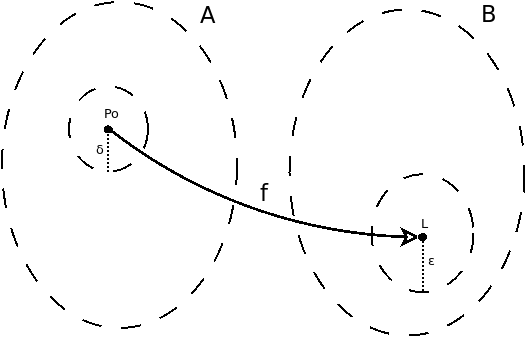
\includegraphics[scale=0.75]{img/teo_fig002_limite.png} 
\centering
\label{fig:limite}
\end{figure}

Como se observa en la figura ~\ref{fig:limite}, el concepto es que, si existe el límite, no importa cuánto se acerque a cero el infinitésimo $\delta$ en el dominio $A$; siempre habrá un entorno centrado en $L$, de radio infinitésimo $\epsilon$, que contenga las imágenes del entorno dominio.

\subsubsection{Aproximación con curva}

\begin{figure}[t]
\caption{Límite}
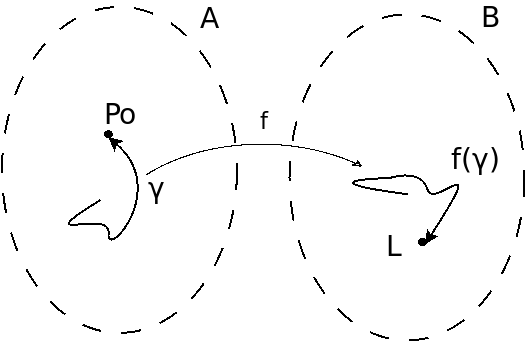
\includegraphics[scale=0.75]{img/teo_fig003_limite_curva.png} 
\centering
\label{fig:limite_curva}
\end{figure}

Lo que pretende mostrar la figura ~\ref{fig:limite_curva} es que, siempre asumiendo que existe el límite, si la aproximación en el dominio se hace con una curva $\gamma$ en lugar de un entorno, la imagen de dicha curva, $f(\gamma)$, convergerá hacia $L$ a medida que $\gamma$ se aproxime a $P_0$. El camino que siga dependerá de cómo transforme f los puntos de $\gamma$.

\subsubsection{Continuidad}

$f$ es continua en $P_0 \longleftrightarrow \displaystyle{\lim_{P \rightarrow P_0}} f(P) = f(P_0)$. En todo otro caso, $f$ es discontinua en $P_0$ de forma \textbf{esencial} si L no existe o es infinito, y de forma \textbf{evitable} si el límite existe, pero $L \neq f(P_0)$ o $\nexists f(P_0)$.

\subsubsection{Unicidad del límite}

Si $L$ existe, es único. Como en Análisis I, esto indica que uno forma de demostrar que un límite no existe, es mostrar que da diferentes valores al calcularlo de diferentes maneras.

\subsubsection{Inexistencia y unicidad}

En funciones de $\Bbb R$ en $\Bbb R$, la existencia e igualdad de los límites laterales garantizaba la existencia del límite, porque sólo había dos direcciones, Sin embargo, en $\Bbb R^n$ hay infinitas formas de aproximarse a un punto; ergo, la igualdad de límites (iterados, radiales, etc) no asegura nada. Sin embargo, si dos difieren, el límite definitivamente no existe.

\subsubsection{Límite de funciones vectoriales}

Para toda función vectorial, el vector límite existe si y sólo si existe el límite para cada uno de los componentes del vector. Por ejemplo:

\begin{equation}
\lim_{t \rightarrow 0} \left( \frac{\sin t}{t}, (1 + t)^\frac{1}{t}, \frac{1-\cos t}{t} \right) = \left( \lim_{t \rightarrow 0} \frac{\sin t}{t}, \lim_{t \rightarrow 0} (1 + t)^\frac{1}{t}, \lim_{t \rightarrow 0} \frac{1-\cos t}{t} \right) = (1, e, 0)
\end{equation}

En este caso, los tres límites existen, y por ende el límite existe. Pero si al menos uno no existiera, dejaría de existir el de la función vectorial.

\subsubsection{Límite de campos escalares}

Ejemplo 1: Sea

\begin{equation}
f(x,y) = x^2 + y
\end{equation}

Es bastante evidente que esta función es continua en todo su dominio; no hay singularidades de ningún tipo. Eso nos permite afirmar, por ejemplo:

\begin{equation}
\lim_{(x,y) \rightarrow (2,1)} f(x,y) = f(2,1) = 5
\end{equation}

Ejemplo 2: Sea

\begin{equation}
f(x,y) = \frac{x^2 - y^2}{x^2 + y^2} \Rightarrow \lim_{(x,y) \rightarrow (0,0)} f(x,y) = ?
\end{equation}

Dado que hay dos variables, no se puede salvar esta indeterminación con elementos de Análisis I como el factoreo y la regla de L'Hopital. En este caso en particular, es posible usar límites sucesivos (no son límites realmente, sino "parientes bastardos"). La idea es variar una sola variable a la vez, dejando el resto constante. Luego, cambiar de variable. Por ejemplo, en $\Bbb R^2$:

\begin{subequations}
\begin{align}
l_{12} = \lim_{y \rightarrow y_0} \left( \lim_{x \rightarrow x_0} f(x,y) \right) \\
l_{21} = \lim_{x \rightarrow x_0} \left( \lim_{y \rightarrow y_0} f(x,y) \right)
\end{align}
\end{subequations}

Nótese que el orden de los subíndices en el nombre indica el orden en que se mueven las variables. Este concepto es fácilmente extendible a n variables. Para el ejemplo anterior, resulta:

\begin{subequations}
\begin{align}
l_{12} = \lim_{y \rightarrow 0} \left( \lim_{x \rightarrow 0} \frac{x^2-y^2}{x^2 + y^2} \right) = \lim_{y \rightarrow 0} \frac{-y^2}{y^2} = -1 \\
l_{21} = \lim_{x \rightarrow 0} \left( \lim_{y \rightarrow 0} \frac{x^2-y^2}{x^2 + y^2} \right) = \lim_{x \rightarrow 0} \frac{x^2}{x^2} = 1
\end{align}
\end{subequations}

Dado que dos límites sucesivos dan valores diferentes, resulta que el límite origen en dos variables no existe.

Cabe destacar que en cada uno de estos pasos, se está calculando el límite para una sola variable, por lo que vale la regla de L'Hopital y demás recursos de una variable.

\section{T4 - Límite 2}

\subsubsection{Límites radiales}

Dado un punto $P_0 = (x_0, y_0)$, la idea es aproximarse infinitesimalmente al mismo a través de las infinitas rectas que lo atraviesan, exceptuando la vertical. Por ejemplo, en $\Bbb R^2$:

\begin{equation}
y = m (x-x_0) + y_0 \Rightarrow l_m = \lim_{x \rightarrow x_0} f(x, m (x-x_0) + y_0)
\end{equation}

Con esta definición, $l_m$ resulta un límite de una variable. Por lo tanto, da como resultado un número, o una expresión que depende de $m$. Como en el segundo caso tendríamos valores diferentes, el límite no existiría. En el primer caso, tendríamos un valor candidato para el límite, pero sin certeza de que exista.

Generalizando para $\Bbb R^n$:

\begin{equation}
P = P_0 + t \overrightarrow{v} \Rightarrow l_{\overrightarrow{v}} = \lim_{t \rightarrow 0} f(P_0 + t \overrightarrow{v})
\end{equation}

\subsubsection{Límites parabólicos}

La misma idea que las rectas, pero usando parábolas. En general, se puede usar cualquier curva que pase por $P_0$. En particular, los límites parabólicos se prestan a funciones cuadráticas o bicuadráticas. Por ejemplo:

\begin{equation}
f(x,y) = \frac{x^2 + y^4}{xy^2} ^ P_0 = (0,0)
\end{equation}

Las curvas a usar serán de la forma $x = a y^2$. Nótese que en este caso particular, por la forma particular de $f$, se eligió $y$ como variable independiente. Con ello resulta:

\begin{equation}
l_p = \lim_{y \rightarrow 0} f(ay^2, y) = \lim_{y \rightarrow 0} \frac{a^2 y^4 + y^4}{ay^2y^2} = \frac{a^2 + 1}{a} \Rightarrow \nexists L
\end{equation}

Este ejemplo da la pauta de que suele ser conveniente elegir curvas de una familia relacionada a las expresiones que aparezcan en $f$; en este caso, cuadrados. Si $f$ contuviera funciones trigonométricas, probablemente ayude aproximarse con senos, cosenos o combinaciones lineales de ellos.

\subsection{Derivada de funciones vectoriales (curvas)}

Sea $\overline{f}:I \rightarrow \Bbb R^n$, con $I \subset \Bbb R$, una curva o función vectorial. La imagen de $\overline{f}$ suele llamarse trayectoria. Si $\overline{f}$ es continua en $I$, es una curva continua. Puede probarse fácilmente que la derivada de una función vectorial es el vector cuyas componentes sean las derivadas de cada función escalar de una variable que componen a $\overline{f}$. Por lo tanto, esto se reduce a derivar una variable (Análisis I).

Una curva se dice de orden $C^p$, o bien que $\overline{f} \in C^p \Longleftrightarrow$ sus derivadas hasta el orden $p$ inclusive son todas continuas. Por ejemplo, si la primera derivada ya es discontinua, $\overline{f} \in C^0$

\section{T5 - Derivadas parciales}

\subsection{Plano normal y recta tangente}

Para una curva $\overline{f}$, el plano normal en un punto $P_0 = \overline{f}(t_0)$ está dado por:

\begin{equation}
\Pi_N : (Q - P_0) \cdot \overline{f}'(t_0) = 0
\end{equation}

Y la recta tangente está dada por:

\begin{equation}
R_T: P_0 + \lambda \overline{f}'(t_0)
\end{equation}

\subsection{Derivadas de campos escalares}

El campo escalar cuyo conjunto de salida es $\Bbb R^2$ es aquel que se denomina impropiamente "de dos variables". Primero, se presentará la definición de derivadas parciales para dicho caso, y luego se generalizará para "n variables". Sean:

\begin{subequations}
\begin{align}
\text{Sea } f: A \rightarrow \Bbb R, \text{ con } A \subseteq \Bbb R^2 / z = f(x,y) \\
\text{Sea } P_0 = (x_0, y_0) \text{ un punto interior de A} \\
\text{Sea } H \text{ un vector de } \Bbb R^2 / (P_0 + H) \in E(P_0, r) \subset A
\end{align}
\end{subequations}

La última definición exige que el vector $P_0 + H$ pertenezca a $A$. Dado todo esto, se definen las derivadas parciales del campo escalar $f$ como los siguientes límites, en tanto existan:

\begin{subequations}
\begin{align}
f_x(x_0, y_0) = \lim_{h \rightarrow 0} \frac{f(x_0 + h, y_0) - f(x_0, y_0)}{h} \\
f_y(x_0, y_0) = \lim_{h \rightarrow 0} \frac{f(x_0, y_0 + h) - f(x_0, y_0)}{h}
\end{align}
\end{subequations}

Notaciones alternativas: $f_x(x_0, y_0) = f'_x(P_0) = D_1 f(P_0) = \frac{\partial f}{\partial x} (P_0)$

Nótese que $f_x$, la derivada parcial respecto a $x$, se calcula incrementado infinitesimalmente sólo $x$, y manteniendo $y$ constante. Lo inverso ocurre para $f_y$.

Generalizando para un campo escalar de $n$ variables:

\begin{equation}
f_{x_i}(P_0) = \frac{\partial f}{\partial x_i} = \lim_{h \rightarrow 0} \frac{f(P_0 + h e_i) - f(P_0)}{h}
\end{equation}

En esta expresión, $e_i$ es un vector de $n$ componentes que valen todas cero, excepto en la i-ésima posición, donde vale 1.

\section{T6 - Derivadas (continuación)}

Para un campo escalar de $n$ variables, las derivadas parciales de orden $k$ son, en total, $n^k$.

\begin{equation}
\text{Nomenclatura:  } f_{xy} = \frac{\partial^2 f}{\partial y \partial x } = \frac{\partial}{\partial y} \left( \frac{\partial f}{\partial x} \right)
\end{equation}

Primero, se deriva respecto de x. Luego, de y. El orden es importante.

\subsection{Teorema de Schwartz}

Para un campo escalar de clase $C^p$ en un punto $P_0$, las derivadas con hasta $p$ subíndices permutados son iguales.

\subsection{Derivada respecto de un vector y derivada direccional}

Sea $f$ un campo escalar y $P_0$ un punto interior del dominio de $f$. Sean $\overrightarrow{v}$ un vector cualquiera en $\Bbb R^n$, y $h$ un escalar tal que $P_0 + h \overrightarrow{v}$ pertenezca a un entorno de $P_0$ incluido en el dominio. Esto puede visualizarse en la figura ~\ref{fig:deriv_direcc} en la página ~\pageref{fig:deriv_direcc}.

\begin{figure}[t]
\centering
\caption{Derivada direccional}
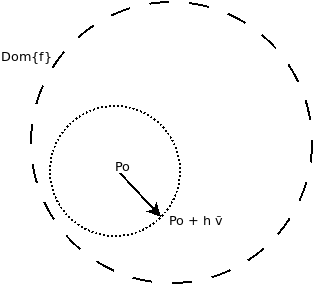
\includegraphics[scale=0.5]{img/teo_fig004_deriv_direcc.png}
\label{fig:deriv_direcc}
\end{figure}

>Entonces, se define la derivada del campo escalar $f$ en el punto $P_0$ respecto del vector $\overrightarrow{v}$ como el siguiente límite, en tanto exista:

\begin{equation}
\tcboxmath[colback=orange!25!white,colframe=orange, title=Derivada respecto de un vector]
{ f'(P_0, \overrightarrow{v}) = \lim_{h \rightarrow 0} \frac{f(P_0 + h \overrightarrow{v})-f(P_0)}{h} }
\end{equation}

Esto es una generalización que incluye a las derivadas parciales como un caso particular. Si $\overrightarrow{v}$ es un versor, la derivada es \textbf{direccional}.

Otra forma de calcular $f'(P_0, \overrightarrow{v})$ involucra una composición de funciones:

% TODO Make this work
% \includegraphics[scale=1]{img/teo_fig005_dd.png} 

Sea $g:\Bbb R \rightarrow \Bbb R / g(t) = f(P_0 + t \overrightarrow{v})$

Derivando:

\begin{equation}
g'(t) = \lim_{h \rightarrow 0} \frac{g(t+h)-g(t)}{h}
\end{equation}

Reemplazando la definición de $g(t)$:

\begin{equation}
g'(t) = \lim_{h \rightarrow 0} \frac{f(P_0 + t \overrightarrow{v} + h \overrightarrow{v}) - f(P_0 + t \overrightarrow{v})}{h}
\end{equation}

Por definición de derivada direccional:

\begin{equation}
f'(P_0 + t \overrightarrow{v}, \overrightarrow{v}) = g'(t) 
\end{equation}

Evaluando en $t = 0$:

\begin{equation}
g'(0) = f'(P_0, \overrightarrow{v})
\end{equation}

\subsection{Diferenciabilidad para campos escalares}

Sean $f$ un campo escalar, $P_0 \in \mathring{A}$, y $\overrightarrow{H} \in \Bbb R^n / (P_0 + \overrightarrow{H}) \in E(P_0, r) \subset A$. Se dice que $f$ es diferenciable en $P_0$ si y sólo si existen una transformación lineal $T_{P_0}: \Bbb R^n \rightarrow \Bbb R$ y una función $\phi_{P_0}: \Bbb R^n \rightarrow \Bbb R / \lim_{\overrightarrow{H} \rightarrow 0} \frac{\phi_{P_0}(\overrightarrow{H})}{||\overrightarrow{H}||} = 0$, que satisfagan:

\begin{equation}
\tcboxmath[colback=orange!25!white,colframe=orange, title=Diferenciabilidad para campo escalar]
{ f(P_0 + \overrightarrow{H}) = f(P_0) + T_{P_0}(\overrightarrow{H}) + \phi_{P_0}(\overrightarrow{H}) }
\end{equation}

\section{T7: Gradiente y diferenciabilidad}

Proposición: Sean $f$ un campo escalar diferenciable en $P_0$, $\overrightarrow{H} = h \overrightarrow{v}$ y $\frac{\phi(\overrightarrow{H})}{||\overrightarrow{H}||} = \psi(\overrightarrow{H})$.

Reemplazando en la definición de diferenciabilidad:

\begin{equation}
f(P_0 + h \overrightarrow{v}) = f(P_0) + \underbrace{ T_{P_0}(h \overrightarrow{v}) }_{\text{Por ser t.l., } h T_{P_0}(\overrightarrow{v})} + \underbrace{ \left|\left|\overrightarrow{H}\right|\right| }_{|h| ||\overrightarrow{v}||} \psi(\overrightarrow{H})
\end{equation}

Restando $f(P_0)$ y dividiendo por $h$ miembro a miembro:

\begin{equation}
\frac{f(P_0 + h\overrightarrow{v})-f(P_0)}{h} = T_{P_0}(\overrightarrow{v}) \pm ||\overrightarrow{v}|| \psi(h \overrightarrow{v})
\end{equation}

Tomando el límite para $h$ tendiendo a cero miembro a miembro:

\begin{equation}
\lim_{h \rightarrow 0} \frac{f(P_0 + h\overrightarrow{v})-f(P_0)}{h} = \lim_{h \rightarrow 0} T_{P_0}(\overrightarrow{v}) \pm \lim_{h \rightarrow 0} ||\overrightarrow{v}|| \psi(h \overrightarrow{v}) 
\end{equation}

Dado que por definición $\psi(\overrightarrow{H}) = \frac{\phi(\overrightarrow{H})}{||\overrightarrow{H}||}$, el segundo sumando del lado derecho tiende a cero. Y el lado izquierdo es la definición de la derivada direccional. Por lo tanto, resulta:

\begin{equation}
f'(P_0, \overrightarrow{v}) = T_{P_0}(\overrightarrow{v})
\end{equation}

Ergo, la transformación lineal de la definición de diferenciabilidad es la derivada direccional. Y además, si un campo escalar es diferenciable, existen todas las derivadas direccionales, lo cual incluye a las derivadas parciales (cuando $\overrightarrow{v}$ es un versor).

\subsection{Vector gradiente y derivada direccional}

Sea un vector genérico $\overrightarrow{H} \in \Bbb R^n$, expresado como matriz de $1xn$ o vector fila $H$:

\begin{equation}
H = \sum\limits_{i=1}^{n} {h_i \overrightarrow{e_i}} \Rightarrow T_{P_0}(H) = \sum\limits_{i=1}^{n}{ h_i \underbrace{T_{P_0}(\overrightarrow{e_i})}_{\text{deriv. parcial } f_{x_i}} } = \sum\limits_{i=1}^{n}{ h_i f_{x_i}(P_0) }
\end{equation}

(Recuérdese de la sección anterior que la transformación lineal $T_{P_0}$ corresponde a la derivada direccional, y para los versores $\overrightarrow{e_i}$ eso corresponde a su vez a las derivadas parciales). La sumatoria final puede ser expresada como un producto escalar entre dos vectores de $\Bbb R^n$:

\begin{align}
    \sum\limits_{i=1}^{n}{ f_{x_i}(P_0) h_i } &= \underbrace{ (f_{x_1}(P_0), f_{x_2}(P_0), \cdots, f_{x_n}(P_0)) }_{ \nabla{f(P_0)} = (\overrightarrow{\nabla{f}}(P_0))^T }
    \begin{pmatrix}
           h_1 \\
           h_2 \\
           \vdots \\
           h_n
    \end{pmatrix}
\end{align}

Entonces, designando a $\overrightarrow{\nabla{f}}(P_0)$ como el vector gradiente evaluado en el punto $P_0$, resulta:

\begin{equation}
T_{P_0}(H) = \underbrace{ \nabla{f}(P_0) H }_{\text{PROD. MATRICIAL}} = \underbrace{ \overrightarrow{\nabla{f}}(P_0) \overrightarrow{H} }_{PROD. ESCALAR}
\end{equation}

\begin{equation}
\tcboxmath[colback=orange!25!white,colframe=orange, title=Gradiente y diferenciabilidad]
{ \text{f es diferenciable} \Leftrightarrow f(P_0 + h) = f(P_0) + \nabla{f}(P_0) H + \phi_{P_0}(H) }
\end{equation}

Despejando $\phi_{P_0}(H)$, dividiendo por $||H||$, tomando norma y exigiendo que el límite del cociente sea cero, resulta:

\begin{equation}
\tcboxmath[colback=orange!25!white,colframe=orange, title=Gradiente y diferenciabilidad]
{ \text{f es diferenciable} \Leftrightarrow \lim_{H \rightarrow \overrightarrow{0}}\frac{ |f(P_0 + h) - f(P_0) - \nabla{f}(P_0) H| }{||H||} = 0 }
\end{equation}

Nótese que la derivada direccional es la proyección del vector gradiente sobre $\overrightarrow{v}$:

\begin{equation}
f'(P_0, \overrightarrow{v}) = \overrightarrow{ \nabla{f} }(P_0) \overrightarrow{v}
\end{equation}

Expresando este producto escalar en función de las normas y el ángulo entre ambos vectores $\alpha$:

\begin{equation}
\overrightarrow{ \nabla{f} }(P_0) \overrightarrow{v} = ||\overrightarrow{ \nabla{f} }(P_0)|| \cos \alpha
\end{equation}

De este modo, la derivada direccional máxima se obtiene cuando $\overrightarrow{v}$ coincide en dirección y sentido con el vector gradiente. Y en ese caso, dicho valor máximo será la norma del vector gradiente. En cuanto al valor mínimo, corresponderá a $\alpha=pi$, y será el opuesto al máximo. Por otro lado, si la derivada direccional es nula, siempre lo será en una dirección perpendicular al gradiente. Ergo, el gradiente en $P_0$ es perpendicular al conjunto de nivel 1 que pasa por $P_0$.

\begin{equation}
f \in C^1 \Rightarrow \text{f es diferenciable} \Rightarrow \left\{
\begin{array}{ll}
\exists \text{ todas las derivadas direccionales} \\
\text{f es continua} \\
\text{Todas las derivadas primeras de f son continuas}
\end{array}
\right.
\end{equation}

Ninguno de los recíprocos es verdadero. Sin embargo, este resultado es útil para aplicar modus tollens. Por ejemplo, si $f$ no es continua, no es diferenciable.

\section{T8 - Derivadas}

\subsection{Interpretación gráfica}

Sea $f$ un campo escalar en $\Bbb R^3$, diferenciable en el punto $P_0$. Por los resultados ya vistos en cuanto a diferenciabilidad, debe cumplirse que:

\begin{equation}
f(P_0 + H) = f(P_0) + \overrightarrow{\nabla{f}}(P_0) H + \theta(H)
\end{equation}

Una posible interpretación gráfica de la derivada sería:

\begin{figure}[ht]
\caption{Interpretación gráfica de la derivada}
\centering
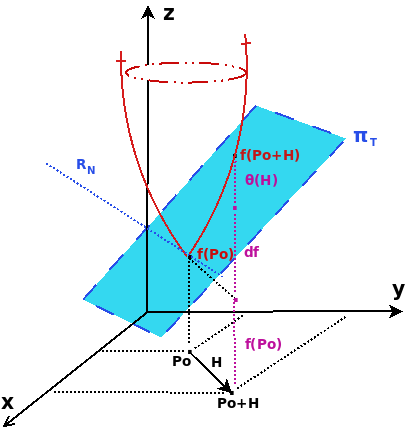
\includegraphics[scale=0.6]{img/teo_fig006_dg.png} 
\label{fig:deriv_graf}
\end{figure}

En lugar de una recta tangente, hay un plano tangente $\Pi_T$ (marcado con color cian en la figura~\ref{fig:deriv_graf}). Dicho plano es geométricamente tangente a la superficie del campo escalar en el punto $P_0$. Una forma directa de determinar el plano tangente es hallar una recta normal $R_N$, que sea ortogonal a la superficie del campo escalar en $P_0$. Dicha recta será la normal que defina el plano tangente en dicho punto.

Observando los segmentos de color fucsia, se observa que $df$ es la distancia entre $f(P_0)$ y el plano tangente. Esto se corresponde al caso de 1 variable, donde $df$ era la distancia entre $f(x_0)$ y la recta tangente. Esto permite hacer una simple extrapolación/aproximación del campo escalar $f$: $f(P_0 + H) \approx f(P_0) + df$. 

Para calcular la expresión del campo tangente, considérese:

\begin{equation}
\Pi_T: z = f(P_0) + \overrightarrow{\nabla{f}}(P_0) H + \theta(H), \text{ siendo } H = (\Delta x, \Delta y) = (x-x_0, y-y_0)
\end{equation}

De forma equivalente:

\begin{gather}
\Pi_T: z-z_0 - f_x(P_0) (x-x_0) - f_y (y-y_0) = 0 \\
R_N = N t + (x_0, y_0, z_0), \text{ siendo } N = (-f_x(P_0), -f_y(P_0), 1)
\end{gather}

Una forma más sencilla:

\begin{equation}
z = f(x,y) \Rightarrow F(x,y,z) \equiv z - f(x,y)
\end{equation}

Siendo el gradiente perpendicular al conjunto de nivel cero, o sea $\nabla{f} \perp (\text{Graf} = C_0(F))$, resulta:

\begin{equation}
\Pi_T: \nabla{F} (P - P_0) = 0, { con } P = (x,y,z)
\end{equation}

\subsection{Derivación de campos vectoriales}

\textbf{Matriz jacobiana de f}: Un campo vectorial $\overline{f}: \Bbb R^n \rightarrow \Bbb R^m$ es diferenciable si:

\begin{gather}
\overline{f}(P_0 + H) = \overline{f}(P_0) + J_f(P_0) H + \theta(H) \\
J_f(P_0) \in \Bbb R^{n x m} / J_{ij} = \frac{\partial f_i}{\partial x_j} 
\end{gather}

La matriz jacobiana $J_f$ puede pensarse como la forma más general de representar una derivada. Cubre el caso de los campos escalares (m = 1) y el caso de 1 variable (n = 1, m = 1).

\section{T9: Derivada de la composición (regla de la cadena)}

Sean $f:\Bbb R^q \rightarrow R^m$ y $g:\Bbb R^n \rightarrow \Bbb R^q$ diferenciables, y en particular sea $f$ diferenciable en el punto $g(x)$. Considérese la función compuesta $h = f \circ g = f(g(x))$. Visualmente:

\begin{figure}[ht]
\caption{Composición de funciones}
\centering
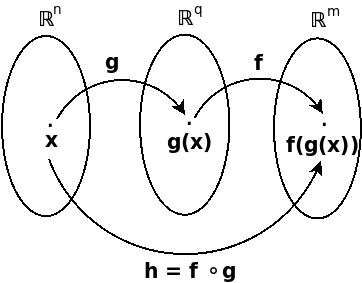
\includegraphics[scale=0.6]{img/teo_fig007_rc.png} 
\label{fig:composic_func}
\end{figure}

La regla de la cadena generalizada establece entonces que:

\begin{gather}
    \tcbhighmath[colframe=orange]{\begin{gathered}\label{equationAB}
      f:\Bbb R^q \rightarrow \Bbb R^m \wedge g:\Bbb R^n \rightarrow \Bbb R^q \text{ son diferenciables }\\
      \Downarrow \\
      h:\Bbb R^n \rightarrow \Bbb R^m / h(x) = f(g(x)) \text{ es diferenciable, y } J_{f \circ g}(x) = J_f(g(x)) J_g (x)
    \end{gathered}}
\end{gather}

Tanto en la composición como en el producto matricial, el orden es relevante.

\subsection{Derivada respecto a una recta}

Esto puede pensarse como una extensión del concepto de derivada direccional, y también como un caso particular de composición de funciones. Sea $f:\Bbb R^n \rightarrow \Bbb R$ diferenciable en el punto $P_0$, y sea la recta parametrizada $\overline{g}(t) = P_0 + t \overrightarrow{v}$, con $\overrightarrow{v} \in \Bbb R^n$. Dicha recta pasa por el punto $P_0$ y tiene su dirección determinada por $\overrightarrow{v}$.

Considérese $h = f \circ g$. Dado que $g:\Bbb R \rightarrow \Bbb R^n$ y $f:\Bbb R^n \rightarrow \Bbb R$, $h:\Bbb R \rightarrow \Bbb R$. Aplicando la regla de la cadena y evaluando en $t=0$, se obtiene un resultado conocido:

\begin{gather}
h'(t) = \overrightarrow{\nabla{f}}(g(t))  \\
h'(0) = \underbrace{ \overrightarrow{\nabla{f}}(P_0) }_{f'(g(0)) = f'(P_0)} \cdot \underbrace{ \overrightarrow{v} }_{ \overrightarrow{g}' }
\end{gather}

En palabras, $h'(0)$ es la derivada direccional de $f$ en el punto $P_0$ y la dirección de $\overrightarrow{v}$.

\subsection{Derivada respecto a una función}

Ya que se puede derivar respecto a una recta, derivar respecto a cualquier otro tipo de función no es otra cosa que derivar una composición de funciones. Por ejemplo, sea $f(x,y) = x^2 y$, que se desea derivar respecto a $y = x^2$. Pensando en términos de una composición:

Pasada a forma paramétrica, la curva $y = x^2$ resulta $\overline{g}(t) = (t, t^2)$. Esto es necesario para que las dimensiones de los dominios e imágenes concuerden y la composición tenga sentido:

\begin{equation}
\left.
\begin{array}{ll}
f:\Bbb R^2 \rightarrow \Bbb R / f(x,y) = x^2 y \\
\overline{g}: \Bbb R \rightarrow \Bbb R^2 / g(t) = (t, t^2)
\end{array}
\right\} \Rightarrow h = f \circ \overline{g} \Rightarrow h'(t) = \underbrace{ \left( \begin{matrix}2t^3 & t^2\end{matrix} \right) }_{J_f(\overline{g}(t))} \underbrace{ \left( \begin{matrix}1 & 2t\end{matrix} \right)^T }_{J_{\overline{g}}(t)} = 4t^3
\end{equation}

\subsection{Derivando por los ``caminitos''}

Esto es un abuso de notación para facilitar el cálculo de derivadas al usar la regla de la cadena.
Sean:

\begin{gather}
f: \Bbb R^3 \rightarrow \Bbb R / f(x, y, z)
g: \Bbb R^2 \rightarrow \Bbb R^3 / \overline{g}(u, v)
h: \Bbb R^2 \rightarrow \Bbb R / h = f \circ g = h(u, v) = f(g(u,v))
\end{gather}

Considérese la derivada de $h$; por la regla de la cadena:

\begin{equation}
h' = J_h = J_f(g) J_g \Rightarrow (h_u h_v) = (f_x f_y f_z) 
\begin{bmatrix}
x_u & x_v \\
y_u & y_v \\
z_u & z_v \\
\end{bmatrix}
\end{equation}

Es en este punto donde se realiza el abuso de notación; se utilizan subíndices y el producto matricial para expresar el orden de derivación a aplicar:

\begin{gather}
h_u = f_x x_u + f_y y_u + f_z z_u = \frac{\partial f}{\partial x} \frac{\partial x}{\partial u} + \frac{\partial f}{\partial y} \frac{\partial y}{\partial u} + \frac{\partial f}{\partial z} \frac{\partial z}{\partial u} \\
h_v = f_x x_v + f_y y_v + f_z z_v = \frac{\partial f}{\partial x} \frac{\partial x}{\partial v} + \frac{\partial f}{\partial y} \frac{\partial y}{\partial v} + \frac{\partial f}{\partial z} \frac{\partial z}{\partial v}
\end{gather}

Los ``caminitos'' que esto representa, visualmente, son:

\begin{figure}[ht]
\caption{Regla de la cadena visualmente}
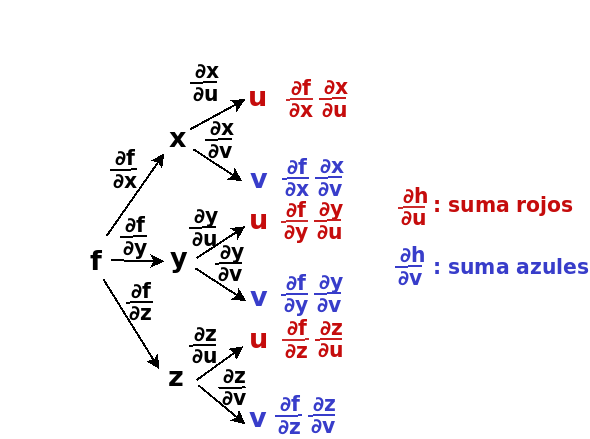
\includegraphics[scale=.5]{img/teo_fig008_rc2.png} 
\centering
\label{fig:rc2}
\end{figure}

\section{T10 - Composición II \& TFI}

\subsection{Composición}

Considérese el siguiente ejemplo de una variable:

\begin{equation}
\left.
\begin{array}{ll}
f(x) = 2x \\
f'(x) = 2
\end{array}
\wedge
\begin{array}{ll}
g(x) = x^2 \\
g'(x) = 2x
\end{array}
\wedge
h = f \circ g
\right\} \Rightarrow
\begin{array}{ll}
h(x) = 4x^2 \\
h'(x) = 8x
\end{array}
\end{equation}

La derivada puede conceptualizarse como el coeficiente de dilatación aplicado a los elementos del dominio (tomando módulo).
Por ejemplo, para $f(x) = 2x$, un intervalo de ancho $a$ en el eje x es mapeado a un intervalo de ancho $2a$ en el eje y; siendo la derivada $f'(x)=2$, esto es trivial. Para el caso más general de las jacobianas, el factor de dilatación está dado por los \textbf{determinantes jacobianos}. Por ejemplo:

\begin{gather}
\overline{f}:\Bbb R^2 \rightarrow \Bbb R^2 / \overline{f}(u,v) = (x(u,v), y(u,v)) \Rightarrow J_f(u,v) =
\begin{bmatrix}
\dfrac{\strut \partial x}{\strut \partial u} & \dfrac{\strut \partial x}{\strut \partial v} \\
\dfrac{\strut \partial y}{\strut \partial u} & \dfrac{\strut \partial y}{\strut \partial v}
\end{bmatrix} = \frac{\partial(x,y)}{\partial(u,v)} \\
|J_f(u,v)| = \frac{\partial x}{\partial u} \frac{\partial y}{\partial v} - \frac{\partial x}{\partial x} \frac{\partial y}{\partial u}
\end{gather}

\subsection{TFI: Teoremas de las funciones implícitas}

\subsubsection{Teorema de Euler}

Definición previa: función homogénea de grado $n$.

\begin{equation}
f:\Bbb R^n \rightarrow \Bbb R^m \text{ es homogénea de grado } k \Leftrightarrow f(\alpha x) = \alpha^k f(x) \text{ } \forall x \in \Bbb R^n
\end{equation}

Con esta definición, el teorema de Euler sobre funciones homogéneas establece que:

\begin{equation}
f:\Bbb R^n \rightarrow \Bbb R \text{ diferenciable en } \Bbb R^n \text{ y homogénea de grado n } \Rightarrow \overrightarrow{x} \cdot \overrightarrow{\nabla f} (\overrightarrow{x}) = n f(\overrightarrow{x})
\end{equation}

\subsubsection{Función implícita}

Supóngase $f:\Bbb R^3 \rightarrow \Bbb R$, definida como $f(x,y,z) = x^2 y^3 - z$. Considérese el conjunto de puntos $(x,y,z) \in \Bbb R^3 /f(x,y,z) = 0$, o en otras palabras el conjunto de nivel cero $C_0$. Una forma alternativa de pensar en este conjunto es como el gráfico de una función $z = \phi(x,y)$, con $Graf \phi = C_0$.

Para este ejemplo, por simple despeje, $z = x^2 y^3$. Pero en la mayoría de los casos tal despeje no es posible; sin embargo, eso no implica que $\phi(x,y)$ no exista. Existe un teorema que permite calcular las derivadas parciales de la función implícita sin conocer su expresión, dadas ciertas condiciones. A saber:

\subsubsection{Teorema de Cauchy-Dini}

Sea $f:\Bbb R^{n+1} \rightarrow \Bbb R$ un campo escalar de clase $C_1$ en el punto $(\overrightarrow{x}, z)$, con $x \in \Bbb R^n$ y $z \in \Bbb R$. Esta notación divide a un punto entre las $n$ coordenadas de $x$, y una coordenada dada por $z$. Si además $f(\overrightarrow{x}, z) = 0$ y $\frac{\partial f}{\partial z} \neq 0$, en un cierto entorno de $\overrightarrow{x}$ existe $z:E(x) \rightarrow \Bbb R / z = \phi(\overrightarrow{x})$. Dicha función implícita $\phi$ satisface $f(\overrightarrow{x}, \phi(\overrightarrow{x})) = 0$. Y por último, las derivadas parciales de $z$ son:

\begin{equation}
z_{x_1} = -\frac{\partial f / \partial x_1}{\partial f / \partial z}, z_{x_2} = -\frac{\partial f / \partial x_2}{\partial f / \partial z}, \ldots
\end{equation}

\subsubsection{Funciones definidas implícitamente por un sistema de ecuaciones}

Por ejemplo, sea el sistema de ecuaciones:

\begin{equation}
\left\{
\begin{array}{ll}
f_1(x, y, z) = 0 \\
f_2(x, y, z) = 0
\end{array}
\right.
\end{equation}

Éste es un sistema de 2 ecuaciones con 3 incógnitas. Por ende, puede decirse que hay un grado de libertad, ya que hay una variable libre, y las otras dos quedan determinadas por ella. Si se toma $x$ como la variable libre, se obtiene:

\begin{equation}
\begin{array}{ll}
y = y(x) \\
z = z(x)
\end{array} \Rightarrow
\left\{
\begin{array}{ll}
f_1(x, y(x), z(x)) = 0 \\
f_2(x, y(x), z(x)) = 0
\end{array}
\right.
\end{equation}

Derivando con la regla de la cadena, miembro a miembro, resulta:

\begin{figure}[ht]
\caption{Derivando un sistema de ecuaciones}
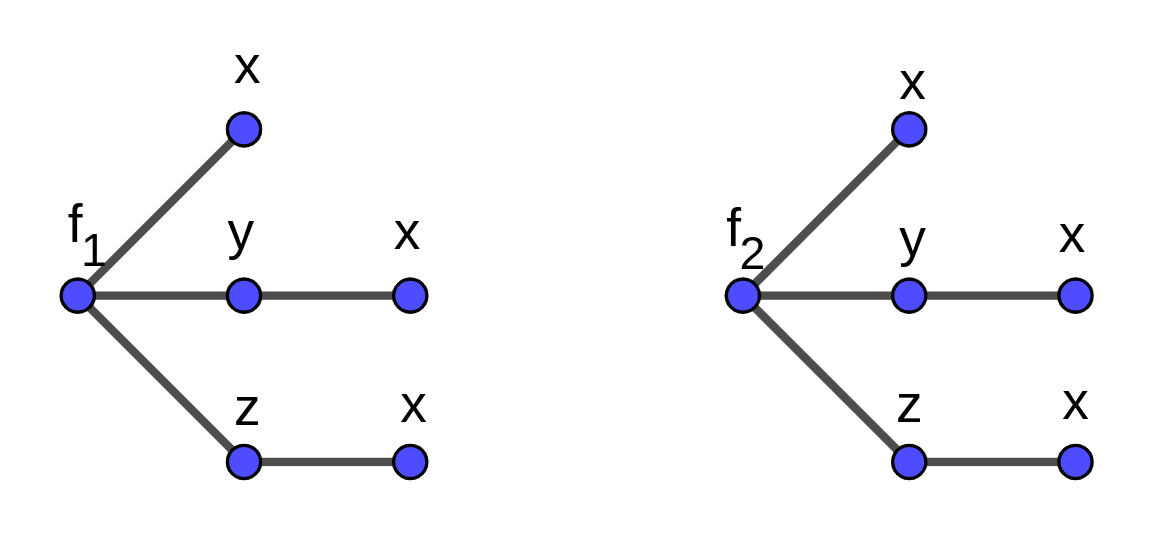
\includegraphics[scale=1]{img/teo_fig009_tcd.png} 
\centering
\label{fig:tcd}
\end{figure}

\begin{equation}
\left\{
\begin{array}{ll}
\frac{\partial f_1}{\partial x} + \frac{\partial f_1}{\partial y} \frac{\mathop{dy}}{\mathop{dx}} + \frac{\partial f_1}{\partial z} \frac{\mathop{dz}}{\mathop{dx}} = 0 \\
\frac{\partial f_2}{\partial x} + \frac{\partial f_2}{\partial y} \frac{\mathop{dy}}{\mathop{dx}} + \frac{\partial f_2}{\partial z} \frac{\mathop{dz}}{\mathop{dx}} = 0
\end{array}
\right.
\end{equation}

Ahora quedan dos ecuaciones con dos incógnitas: $\frac{\mathop{dy}}{\mathop{dx}}$ y $\frac{\mathop{dz}}{\mathop{dx}}$. Pasando $\frac{\partial f_1}{\partial x}$ y $\frac{\partial f_2}{\partial x}$ como términos independientes y expresando matricialmente:

\begin{equation}
\left\{
\begin{array}{ll}
\frac{\partial f_1}{\partial y} \frac{\mathop{dy}}{\mathop{dx}} + \frac{\partial f_1}{\partial z} \frac{\mathop{dz}}{\mathop{dx}} = -\frac{\partial f_1}{\partial x} \\
\frac{\partial f_2}{\partial y} \frac{\mathop{dy}}{\mathop{dx}} + \frac{\partial f_2}{\partial z} \frac{\mathop{dz}}{\mathop{dx}} = -\frac{\partial f_1}{\partial x}
\end{array}
\right. \approx 
\underbrace{
\begin{bmatrix}
\frac{\partial f_1}{\partial y} & \frac{\partial f_1}{\partial z} \\
\frac{\partial f_2}{\partial y} & \frac{\partial f_2}{\partial z}
\end{bmatrix}
}_{A`}
\begin{bmatrix}
\mathop{dy}/\mathop{dx} \\
\mathop{dz}/\mathop{dx}
\end{bmatrix} = 
\begin{bmatrix}
-\partial f_1/ \partial x \\
-\partial f_2/ \partial x
\end{bmatrix}
\end{equation}

Para que este sistema sea determinado, o en otras palabras, para que existan $\frac{\mathop{dy}}{\mathop{dx}}$ y $\frac{\mathop{dz}}{\mathop{dx}}$, el determinante de la matriz $A$ debe ser no nulo.

\subsubsection{Teorema de Cauchy-Dini generalizado}

Sea $\overline{f}:\Bbb R^{n+m} \rightarrow \Bbb R^m$, $\overline{f} = (f_1, f_2, \ldots, f_m)$. Vale decir, un campo vectorial compuesto por $m$ campos escalares de $n$ variables. Sea $f_i(\overrightarrow{x}, \overrightarrow{z}) = 0$, donde $\overrightarrow{x} \in \Bbb R^n$ corresponde a las variables libres, y $\overrightarrow{z} \in \Bbb R^m$ corresponde a las variables dependientes. De la condición de igualdad a cero surge un sistema de ecuaciones al aplicar el teorema de Cauchy-Dini a cada campo escalar. En dicho sistema, las incógnitas son $\frac{\partial z_k}{\partial x_h}$, donde $k = 1, 2, \ldots, m$ y $h = 1, 2, \ldots, n$.

\section{T11 - Taylor}

Para una variable:

\begin{equation}
g(x_0 + h) = \underbrace{ g(x_0) + g'(x_0) h + \frac{1}{2!} g''(x_0) h^2 + \ldots + \frac{1}{n!} g^{(n)}(x_0) h^n }_{P_n(x_0)} +  \underbrace{ \frac{1}{(n+1)!} g^{(n+1)}(c) h^{n+1} }_{T_n(x_0, c)}
\end{equation}

$P_n(x_0)$ es el polinomio de Taylor de grado $n$ desarrollado en el punto $x_0$. Dicho punto suele denominarse como centro del desarrollo. El término $T_n(x_0, c)$ es el resto o término complementario; es importante recordar que se evalúa en $c \in (x_0, x_0 + h)$ y no en $x_0$.

Una importante consecuencia del teorema de Taylor es que si $g$ es infinitamente derivable, y se conocen todas sus derivadas en un punto, se puede extrapolar la función completa sólo con un punto. También es posible tomar más de un punto de desarrollo, para disminuir el error.

El teorema de Taylor de 1 variable puede reescribirse en términos del diferencial en lugar de la derivada. Puede demostrarse que esa definición es válida para $n$ variables.

\begin{equation}
\tcboxmath[colback=orange!25!white,colframe=orange, title=Taylor generalizado]
{ g(x_0 + h) = g(x_0) + dg(x_0) h + \ldots + \frac{1}{n!} d^{(n)}g(x_0) +  \frac{1}{(n+1)!} d^{(n+1)}g(c) }
\end{equation}

Nótese que las potencias de $h$ se fueron. En dicha expresión, $d^ng$ es el n-ésimo diferencial de $g$. Para campos escalares:

\begin{equation}
d^{n}f(P_0, \overrightarrow{H}) = \left. (\overrightarrow{H} \cdot \overrightarrow{\nabla f})^n \right|_{P_0}
\end{equation}

El producto entre $\overrightarrow{H}$ y el gradiente es escalar, y se evalúa en $P_0$. De esa manera, el teorema de Taylor para campos escalares de $n$ variables resulta:

Para un campo escalar $f \in C^{n+1}$ en un entorno de $P_0$, y para $H \in \Bbb R^n/ (P_0+ H)$ pertenece a un entorno de $P_0$ incluido en $Dom f$:

\begin{equation}
f(P_0+H) = f(P_0) + df(Po, H) + \ldots + \frac{1}{n!} d^nf(Po,H) + \frac{1}{(n+1)!} d^{n+1}f(c)
\end{equation}

\subsection{Extremos de campos escalares}

\noindent
\begin{minipage}{\textwidth}
\centering
\captionof{figure}{Extremo de campo escalar tipo 1}
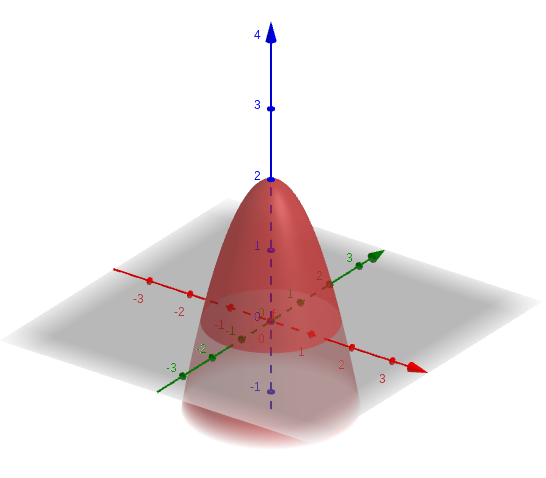
\includegraphics[scale=0.6]{img/teo_fig010_exce01.png} 
\label{fig:exce01}
\end{minipage}

Sea $P_0$ un punto interior del dominio de $f$, y sea:

\begin{equation}
E(P_0) \subset Dom f / f(P) \leq f(P_0) \forall P \in E(P_0)
\end{equation}

Entonces, $P_0$ es un máximo local. Es un escalar, y se alcanza en $P_0$. Este es el caso tipo 1, correspondiente a la figura~\ref{fig:exce01}. 

\begin{figure}[ht]
\caption{Extremo de campo escalar tipo 2}
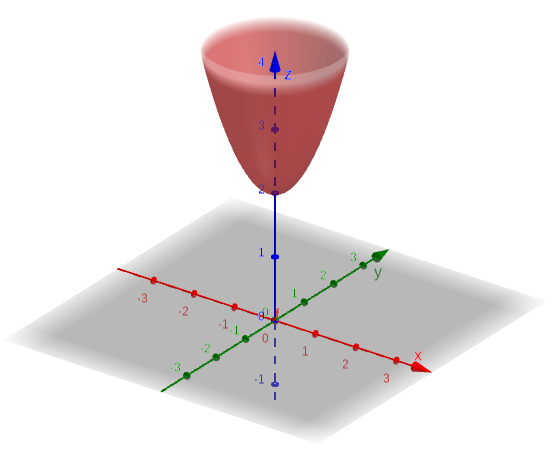
\includegraphics[scale=0.6]{img/teo_fig010_exce02.png} 
\centering
\label{fig:exce02}
\end{figure}

El caso 2, ejemplificado en la figura~\ref{fig:exce02}, se define igual que el 1, cambiando el $\leq$ por $\geq$, y ``máximo local'' por ``mínimo local''

\begin{figure}[ht]
\caption{Extremo de campo escalar tipo 3}
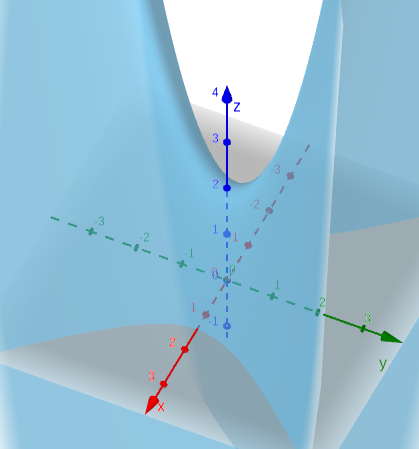
\includegraphics[scale=0.6]{img/teo_fig010_exce03.png} 
\centering
\label{fig:exce03}
\end{figure}

El caso 3, ejemplificado en la figura~\ref{fig:exce03}, se denomina \textbf{punto silla}, y se define de la siguiente manera:

Si $\forall E(P_0) \in P / f(P) \geq f(P_0)$, existen puntos $P' / f(P') \leq f(P_0)$, y además $f$ es diferenciable en $P_0$ con diferencial nulo en dicho punto $\Rightarrow$ el punto $(P_0, f(P_0))$ es un punto silla.

\textbf{Teorema}: Sea $f$ diferenciable en $P_0$, y $(P_0, f(P_0))$ un extremo local $\Rightarrow$ todas las derivadas parciales son nulas en $P_0$ $\Rightarrow \overrightarrow{\nabla f}(P_0) = 0$.

Nótese que la condición es necesaria, pero no suficiente. La anulación total del gradiente en un punto no garantiza que el mismo sea un extremo local, pero en todo extremo local se anula el gradiente.

\section{T12 - Extremos, 2da parte}

Otra forma más general de expresar la condición de diferenciabilidad es:

\begin{equation}
f(P_0 + H) = f(P_0) + J_f(P_0) H + \frac{1}{2} H^T H_f(P_0) H + \sigma( ||H||^2 )
\label{eq:hessiandiff}
\end{equation}

En la ecuación~\ref{eq:hessiandiff}, $H_f$ es la matriz de Hesse, o Hessiano: $H_{f_{ij}} = \frac{\partial^2 f}{\partial x_j \partial x_i}$. Así como el jacobiano está asociado a las derivadas parciales de primer orden, el hessiano agrupa las derivadas de segundo orden mixtas. Por ello se entiende las que no se hacen derivando dos veces la misma variable.

El último término es una forma abreviada del infinitésimo que aparecía en la definición inicial de diferenciabilidad:

\begin{equation}
\sigma(||H||^2) = \frac{\phi(H)}{||H||^2}, \lim_{H \rightarrow 0}  \sigma(||H||^2) = 0
\end{equation}

Si $P_0$ es un extremo local y $f \in C^3$, el término del jacobiano se anula, y resulta:

\begin{equation}
f(P_0 + H) = f(P_0) + \frac{1}{2} H^T H_f(P_0) H + \sigma(||H||^2)
\end{equation}

Sea:

\begin{equation}
g:\Bbb R^n \rightarrow \Bbb R / g(H) = \frac{1}{2} H^T H_f(P_0) H
\end{equation}

Por las dimensiones de los dos vectores y la matriz, el producto da siempre un escalar. La función $g$ es una \textbf{forma cuadrática} en $\Bbb R^n$ que se dice \textbf{definida positiva (o negativa)} según sea $g(H) > 0$ (o $g(H) < 0$) para todo $H \neq 0$.  

Si se considera el subconjunto de $\Bbb R^n / ||H|| = 1$ y se restringe $g$ a ese conjunto, debe alcanzarse un mínimo $m$. Ergo, en $P_0$ se alcanza un mínimo local si $g$ es definida positiva, un máximo si $g$ es definida negativa, y un punto silla si es indefinida. En el caso de que sea nula, se requiere otro análisis. Recuérdese que en todo este análisis, $P_0$ es un candidato a extremo local por anularse el jacobiano en él.

g es definida positiva $\Leftrightarrow$ todos los determinantes diagonales de $H(P_0)$ son positivos

g es definida negativa $\Leftrightarrow$ todos los determinantes diagonales de orden impar de $H(P_0)$ son negativos, y los de orden par son positivos

g es indefinida $\Leftrightarrow$ no es definida positiva ni negativa

\subsection{Determinantes diagonales}

Para explicar a través de un ejemplo, considérese una matriz de 4x4 con elementos $a, b, c, \ldots , $ñ dispuestos por filas:

\begin{figure}[ht]
\caption{Determinantes diagonales}
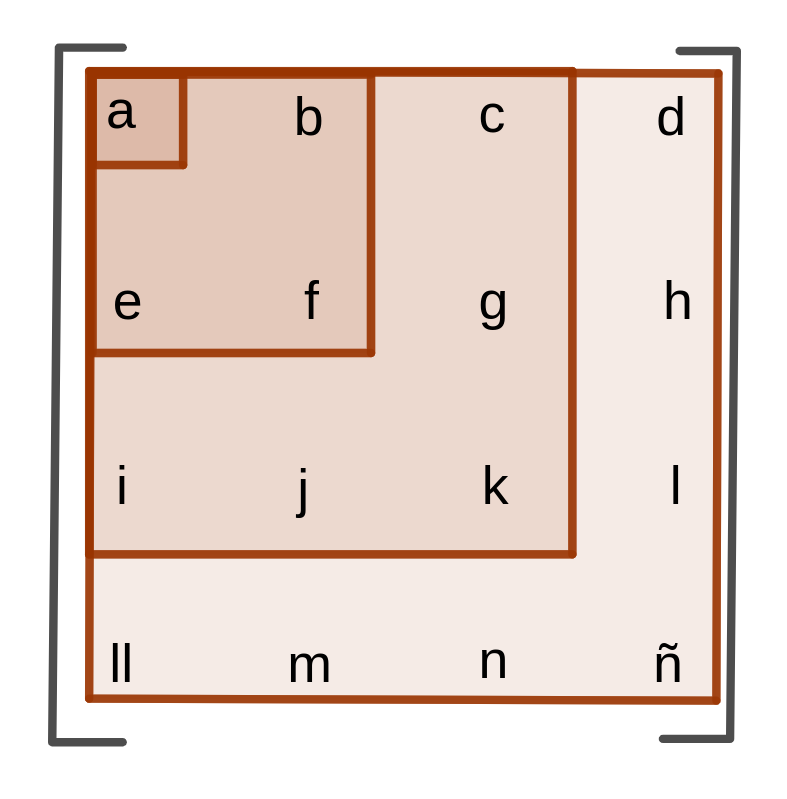
\includegraphics[scale=0.8]{img/teo_fig011_detdiag.png} 
\centering
\label{fig:detdiag}
\end{figure}

\begin{gather}
\det_1 = \det [a] = a \\
\det_2 = \det \begin{bmatrix} a & b \\ e & f \end{bmatrix} = a f - b e \\
\det_3 = \det \begin{bmatrix} a & b & c \\ e & f & g \\ i & j & k \end{bmatrix} \\
\det_4 = \det \begin{bmatrix} a & b & c & d \\ e & f & g & h \\ i & j & k & l \\ ll & m & n & \tilde{n} \end{bmatrix}
\end{gather}

Generalizando, $\det_i$ se obtiene tomando una submatriz cuadrada de tamaño $i$ cuyo primer elemento siempre coincide con el primer elemento de la matriz original. El subíndice $i$ va de $1$ a $n$, siendo $\det_n$ equivalente al determinante de la matriz completa.

Volviendo al tema de si $g$ es definida positiva o negativa, si la matriz del ejemplo fuera $H(P_0)$:

$g$ es definida positiva y hay un mínimo local en $P_0$ si $\det_i > 0 \forall i \in (1 \ldots 4)$

$g$ es definida negativa y hay un máximo local en $P_0$ si $\det_1 < 0, \det_2 > 0, \det_3 < 0, \det_4 > 0$. Vale decir, todos los impares negativos, y todos los pares positivos.

En cualquier otro caso, $g$ es indefinida. Si no ocurre que todos los determinantes diagonales son nulos, entonces $P_0$ es un punto silla.

\subsection{Extremos condicionados}

Sea un campo escalar de $n$ variables $z = F(x_1, x_2, \ldots, x_n)$ con $m$ condiciones de vínculo de la forma $G(x_1, x_2, \ldots, x_n) = 0$. Se define una función auxiliar $H$, cuyos extremos son los de $F$ restringida por las condiciones $G$. De forma general:

\begin{equation}
H(x_1, x_2, \ldots, x_n; \lambda_1, \lambda_2, \ldots, \lambda_m) = F(x_1, x_2, \ldots, x_n) + \sum\limits_{i=1}^m \lambda_i G_i(x_1, x_2, \ldots, x_n) 
\end{equation}

Los escalares $\lambda_i$ se denominan \textbf{multiplicadores de Lagrange}, y son los valores a determinar para resolver un problema de extremos condicionados.

Por ejemplo, sea $F(x,y) = 3 x^2 + y^2 - x + 1$, y se desea hallar sus extremos sobre la curva $x^2 + \frac{y^2}{4} = 1$. La curva determina la única condición de vínculo $G(x,y) = x^2 + \frac{y^2}{4} - 1$. La función auxiliar $H$ resulta:

\begin{equation}
H(x, y, \lambda) = 3 x^2 + y^2 - x + 1 + \lambda \left( x^2 + \frac{y^2}{4} - 1 \right)
\end{equation}

El próximo paso es hallar los puntos críticos de $H$. Para ello, se buscan los ceros del gradiente, o lo que es lo mismo, de las derivadas parciales en cada componente:

\begin{equation}
\left\{
\begin{array}{ll}
H_x = 6 x - 1 + 2 \lambda x \\
H_y = 2 y + \frac{1}{2} \lambda y \\
H_{\lambda} = x^2 + \frac{y^2}{4} - 1
\end{array}
\right.
\end{equation}

En las ecuaciones que tienen $\lambda$, conviene despejarlo primero, porque es el que primero interesa restringir:

\begin{equation}
\begin{array}{ll}
H_x = 0 \Leftrightarrow \lambda = \frac{1-6x}{2x} \\
H_y = 0 \Leftrightarrow \lambda = -4, \text{ con } y \neq 0
\end{array}
\end{equation}

Fijado $\lambda = -4$, reemplazando en la primera ecuación, se obtiene $x = -\frac{1}{2}$. Ingresando $x$ en la tercera ecuación, resulta $y = \pm \sqrt{3}$. Esto da dos posibles puntos críticos: $(-\frac{1}{2}, \sqrt{3})$ y $(-\frac{1}{2}, -\sqrt{3})$

Considerando el caso $y = 0$, que había sido apartado al calcular $\lambda$, se verifica que $x^2 = 1$ anula todas las derivadas. Por lo tanto, hay dos puntos críticos posibles más: $(1, 0)$ y $(-1, 0)$.

Para categorizar los posibles puntos críticos, queda como ejercicio analizar el hessiano de la función auxiliar $H$ en dichos puntos.

\section{T13 - Integrales}

\subsection{Integral de línea o circulación}

Sean $\overrightarrow{f}$ un campo vectorial $\in C^0$, y $\overrightarrow{\beta}$ una curva uniparamétrica $\in C^1$ cuyos puntos sean de igual dimensión que los del dominio de $f$. La integral de línea de $\overrightarrow{f}$ sobre $\overrightarrow{\beta}$ se define entonces como:

\begin{equation}
\int_{\overrightarrow{\beta}} \overrightarrow{f} d\overrightarrow{\beta} = \int_{a}^{b} \overrightarrow{f}(\overrightarrow{\beta}(t)) \underbrace{\cdot}_{prod. escalar} \underbrace{ \beta '(t) \mathop{dt} }_{d\overrightarrow{\beta}}
\end{equation}

Los valores $a$ y $b$ corresponde a los puntos inicial y final de la curva $\overrightarrow{\beta}$. No es trivial ver el sentido geométrico de la integral en este caso, pero tiene muchas aplicaciones, como por ejemplo calcular flujo magnético.

\subsection{Integral de trayectoria}

Sean ahora $f$ un campo escalar $\in C^0$, y $\overrightarrow{r}$ una curva uniparamétrica $\in C^1$ cuyos puntos sean de igual dimensión que los del dominio de $f$. Se define entonces la integral de trayectoria como:

\begin{equation}
\int_{\overrightarrow{r}} f(\overrightarrow{r}) d\overrightarrow{r} = \int_{a}^{b} f(\overrightarrow{r(t)}) ||r'(t)|| \mathop{dt}
\end{equation}

Nuevamente, $a$ y $b$ son los valores del parámetro $t$ asociados al punto inicial y final de $r$, respectivamente. Nótese que el integrando es directamente un número real en este caso (en el otro también, pero hay que realizar un producto escalar primero).

En este caso, sí hay una interpretación geométrica directa de la integral, al menos para $\Bbb R^3$. Si el dominio de $f$ es $\Bbb R^2$, y su gráfico $z = f(x,y)$ una superficie en $\Bbb R^3$, y $r$ es una curva en $\Bbb R^3$, la integral de línea de $f$ sobre $r$ es el área bajo la curva $r$ a lo largo del gráfico de $f$.

\begin{figure}[ht]
\caption{Integral de línea en $\Bbb R^3$}
\centering
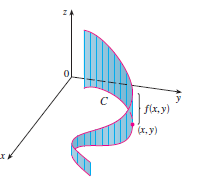
\includegraphics[scale=0.6]{img/teo_fig012_li.png} 
\end{figure}

Por lo tanto, una aplicación inmediata de esta integral es el cálculo del área de superficies curvas.

\subsection{Invirtiendo el sentido de circulación}

Para hacerlo manteniendo fijos $a$ y $b$:

\begin{align}
\overrightarrow{\beta} &: [a, b] \rightarrow \Bbb R^n \\
\overrightarrow{\sigma} &: [a, b] \rightarrow \Bbb R^n / \overrightarrow{\sigma}(t) = \overrightarrow{\beta}(a + b - t) 
\end{align}

\subsection{Observaciones}

\textbf{1)} Si el campo escalar de la integral de trayectoria es la constante 1, el resultado de la integral es la longitud de la curva. Por ejemplo, se sabe que la longitud de la circunferencia es $2 \pi r$. Integrando una curva que represente un círculo de radio $r$:

\begin{align}
\overrightarrow{r(t)} &= (r \cos t, r \sin t) \Rightarrow \int_{\overrightarrow{r}} 1 \mathop{d\overrightarrow{r}} = \int_{0}^{2 \pi} ||r'(t)|| \mathop{dt} = \int_{0}^{2 \pi} ||(-r \sin t, r \cos t)|| \mathop{dt} \\
&= \int_{0}^{2 \pi} \sqrt{r^2 \sin^2 (t) + r^2 \cos^2 (t)} \mathop{dt} = r \int_{0}^{2 \pi} \underbrace{ \sqrt{\sin^2(t) + \cos^2(t)} }_{1} \mathop{dt} = r \int_{0}^{2 \pi} \mathop{dt} \\
&= r (2 \pi - 0) = 2 \pi r
\end{align}

\textbf{2)} Ambos tipos de integral (de línea y de trayectoria) están igualmente bien definidas para curvas $C^1$ a trozos, o seccionalmente $C^1$. La integral simplemente se calcula para cada sección de curva, y se suman los resultados.

\begin{equation}
\left.
\begin{array}{ll}
\beta = \bigcup\limits_{i=1}^p \beta_i, \text{ con } \beta_i \in C^1 \\
\beta_i: [a_i, b_i] \rightarrow \Bbb R^n \\
\beta_{i}(b_i) = \beta_{i+1}(a_{i+1})
\end{array}
\right\} \Rightarrow
\left\{
\begin{array}{ll}
\int_{\overrightarrow{\beta}} \overrightarrow{f} d\overrightarrow{\beta} = \sum\limits_{i=1}^p \int_{\overrightarrow{\beta_i}} \overrightarrow{f} d\overrightarrow{\beta_i} \\
\int_{\overrightarrow{\beta}} f d\overrightarrow{\beta} = \sum\limits_{i=1}^p \int_{\overrightarrow{\beta_i}} f d\overrightarrow{\beta_i}
\end{array}
\right.
\end{equation}

\textbf{3)} Para curvas cerradas, el sentido de circulación se define:

\begin{itemize}
\item Positivo si a la izquierda está el interior: $\oint_{\beta^+}$
\item Negativo si a la derecha está el interior: $\oint_{\beta^-}$
\end{itemize}

\textbf{4)} Curva simple = curva inyectiva. La inyectividad se considera mirando la curva parametrizada: cada valor de $t$ debe corresponder a un punto distinto. Por lo tanto, si la curva pasa más de una vez por el mismo punto, ya no es simple/inyectiva. Otra forma de llamar a las curvas no simples es \textbf{lazo} o \textbf{rulo}. Un lazo es \textbf{simple} si tiene un solo punto no inyectivo.

\textbf{5)} Un lazo simple también se denomina \textbf{lazo de Jordan}. El \textbf{Teorema de Jordan} establece que todo lazo divide el plano en dos regiones: una acotada (el interior) y otra no acotada (el exterior). El símbolo de infinito es un lazo no simple; aunque sea el mismo punto, se pasa dos veces por él, ergo no es simple.

\textbf{6)} Nomenclatura para campos vectoriales de 3 componentes:

Sean:

\begin{align}
\overrightarrow{f}(x, y, z) &= (P(x,y,z), Q(x,y,z), R(x, y, z)) \\
\overrightarrow{\beta}(t) &= (x(t), y(t), z(t))
\end{align}

Entonces, la integral de línea resulta:

\begin{align}
\int_{\overrightarrow{\beta}} \overrightarrow{f} d\overrightarrow{\beta} &= \int_{a}^{b} \overrightarrow{f}(\overrightarrow{\beta}(t)) \cdot \beta'(t) \mathop{dt} \\
&= \int_{a}^{b} \begin{bmatrix}P(\overrightarrow{\beta(t)}) & Q(\overrightarrow{\beta(t)}) & R(\overrightarrow{\beta(t)})\end{bmatrix} \cdot \begin{bmatrix}x'(t) \\ y'(t) \\ z'(t)\end{bmatrix} \mathop{dt} \\
&= \int_{a}^{b} P(\overrightarrow{\beta(t)}) \underbrace{x'(t) \mathop{dt}}_{\mathop{dx}} + Q(\overrightarrow{\beta(t)}) \underbrace{y'(t) \mathop{dt}}_{\mathop{dy}} + R(\overrightarrow{\beta(t)}) \underbrace{z'(t) \mathop{dt}}_{\mathop{dz}}
\end{align}

Realizando un potencial abuso de notación:

\begin{equation}
\int_{\overrightarrow{\beta}} \overrightarrow{f} d\overrightarrow{\beta} = \int_{\overrightarrow{\beta}} P \mathop{dx} + Q \mathop{dy} + R \mathop{dz}
\end{equation}

\textbf{7)} Una integral de línea puede ser interpretada como una de trayectoria. Verbigracia:

Sea:

\begin{equation}
\overrightarrow{T}(t) = \frac{ \overrightarrow{\beta}'(t) }{||\overrightarrow{\beta}'(t)||}
\end{equation}

Entonces, considérese la integral de línea de un campo vectorial $\overrightarrow{F}$ sobre la curva $\overrightarrow{\beta}$:

\begin{align}
\int_{\overrightarrow{\overrightarrow{\beta}}} \overrightarrow{F} \cdot d\overrightarrow{\beta} &= \int_{a}^b \overrightarrow{F}(\overrightarrow{\beta}(t)) \cdot \overrightarrow{\beta'(t)} \mathop{dt} = \int_{a}^b \left[ \overrightarrow{F}(\overrightarrow{\beta}(t)) \cdot \frac{ \overrightarrow{\beta'(t)} }{||\overrightarrow{\beta'(t)}||} \right] ||\overrightarrow{\beta'(t)}|| \mathop{dt} \\
&= \int_{a}^b \left[ \overrightarrow{F}(\overrightarrow{\beta}(t)) \cdot \overrightarrow{T}(t) \right] ||\overrightarrow{\beta}'(t)|| \mathop{dt}
\end{align}

Si se define el campo escalar $H = \overrightarrow{F}(\overrightarrow{\beta}) \cdot \overrightarrow{T}$, la integral de trayectoria de $H$ es igual a la integral de línea de $F$, ambas sobre la misma curva $\overrightarrow{\beta}$, claro.

\section{T14 - Integrales II}

\subsection{Reparametrización}

Reparametrizar una curva es simplemente expresarla de otra manera equivalente. Los valores iniciales del parámetro y las expresiones de los componentes pueden ser diferentes, pero deben generar exactamente los mismo puntos que componen la curva.

Es de interés hallar las condiciones que debe cumplir una reparametrización para no cambiar el valor de la integral de línea. Se presentarán dichas condiciones como resultados.

Sea una función $\phi:\Bbb R \rightarrow \Bbb R$ que satisface:

\begin{align}
&\phi:[a, b] \rightarrow [a^*, b^*] \\
&\phi \text{ es biyectiva en el intervalo } [a,b] \\
&\phi \in C^1[a,b] \\
&\phi(a) = a^* \wedge \phi(b) = b^* \\
&\phi'(t) > 0 \text{ } \forall \text{ } t \in [a,b]
\end{align}

Con estas condiciones, $\phi$ es un \textbf{diffeormorfismo} en $\Bbb R^2$. Una función es un diffeomorfismo si es biyectiva y diferenciable, y su inversa también es diferenciable. Las condiciones cumplidas por $\phi$ garantizan esto, siendo suficientes pero no necesarias. 

Por otro lado, sea $\overrightarrow{\sigma}$ una función que satisface:

\begin{align}
&\sigma: [a^*, b^*] \rightarrow \Bbb R^n \\
&\sigma\in C^1[a^*, b^*] \\
&\sigma(a^*) = A \wedge \sigma(b^*) = B
\end{align}

Finalmente, sea $\overrightarrow{H} = \overrightarrow{\sigma} \circ \phi$. La función $\overrightarrow{H}$ es una reparametrización; $\phi$ es la función que mapea el intervalo parámetrico original $[a,b]$ en el nuevo intervalo $[a^*, b^*]$, y $\sigma$ es la nueva expresión de la curva original $\beta$. Para visualizar las relaciones entre estas funciones, obsérvese la figura~\ref{fig:reparam}.

\begin{figure}[ht]
\centering
\caption{Reparametrización}
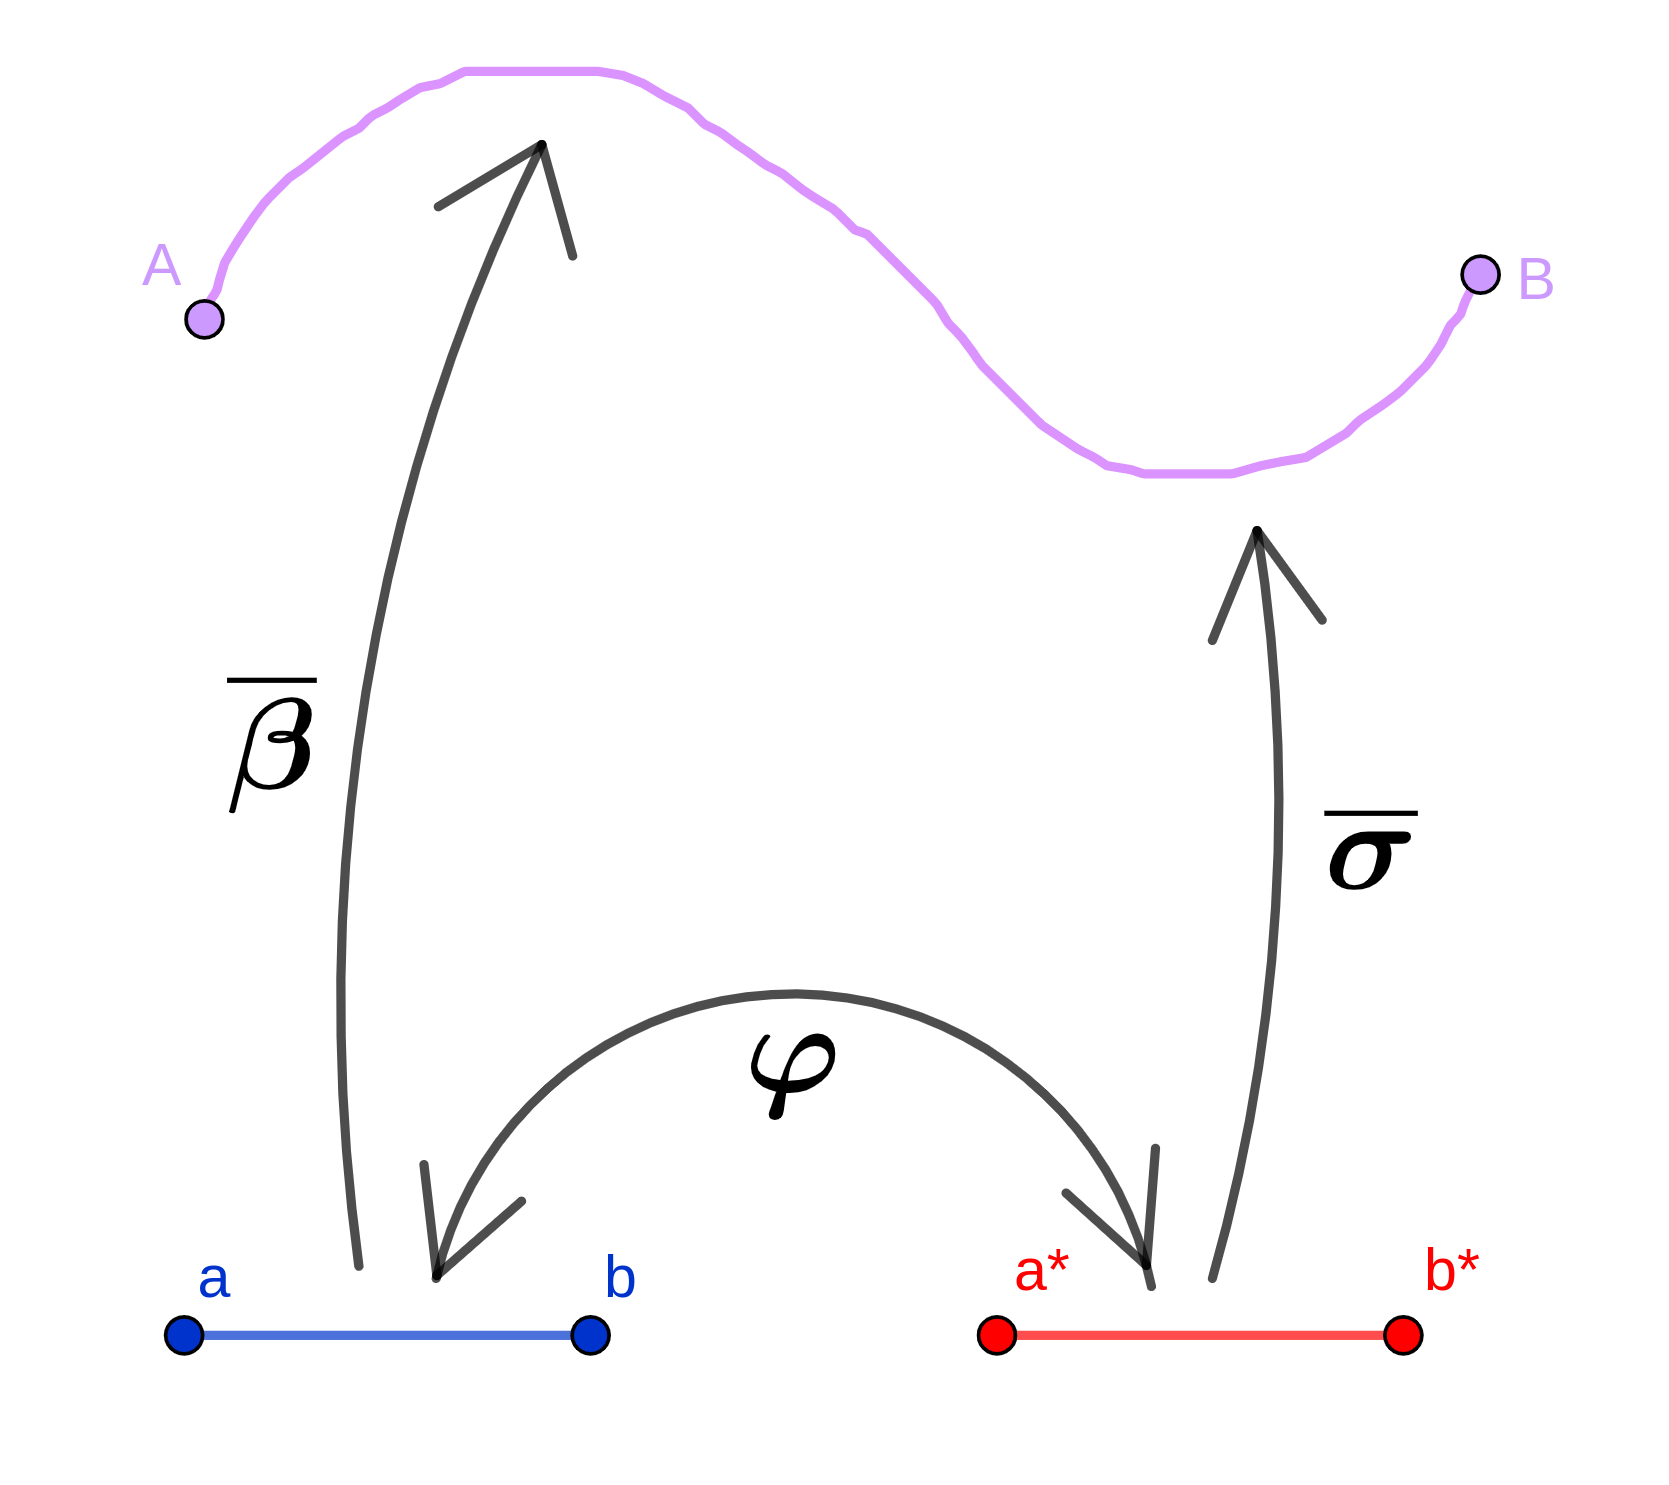
\includegraphics[scale=0.7]{img/teo_fig013_re.png}
\label{fig:reparam}
\end{figure}

Si $\phi$ y $\overrightarrow{\sigma}$ cumplen las condiciones detalladas, entonces puede demostrarse que $\overrightarrow{H}$ es una parametrización equivalente de la curva, y el valor de la integral de línea sobre cualquier campo vectorial se conservará.

\subsection{Preservación del signo}

La integral de línea es invariante frente a diffeomorfismos que preserven el sentido del recorrido. En cambio, la integral de trayectoria se preserva para cualquier diffeomorfismo.

Si $\sigma_1$ es equivalente a $\sigma$ pero invierte el sentido de recorrido:

\begin{gather}
\int_{\overrightarrow{\sigma_1}} \overrightarrow{f} d\overrightarrow{\sigma_1} = - \int_{\overrightarrow{\sigma}} \overrightarrow{f} d\overrightarrow{\sigma} \\
\int_{\overrightarrow{\sigma_1}} f d\sigma_1 = \int_{\overrightarrow{\sigma}} f d\sigma
\end{gather}

Ergo, para integrales de línea, cambiar el sentido de recorrido de la curva cambia el signo de la integral, de forma análoga a cuando en integrales de 1 variable se cambiaba el orden de los límites de la integral. Esto tiene sentido porque para los vectores el sentido es importante, pero no para los escalares.

\subsection{Integral de línea y campos conservativos}

\textbf{Lema}: Sean $\Phi$ un campo escalar diferenciable en un dominio $D_{\Phi}$, y sea $\sigma$ una curva $C^1$ contenida en dicho dominio. 

\begin{figure}[ht]
\centering
\caption{Lema}
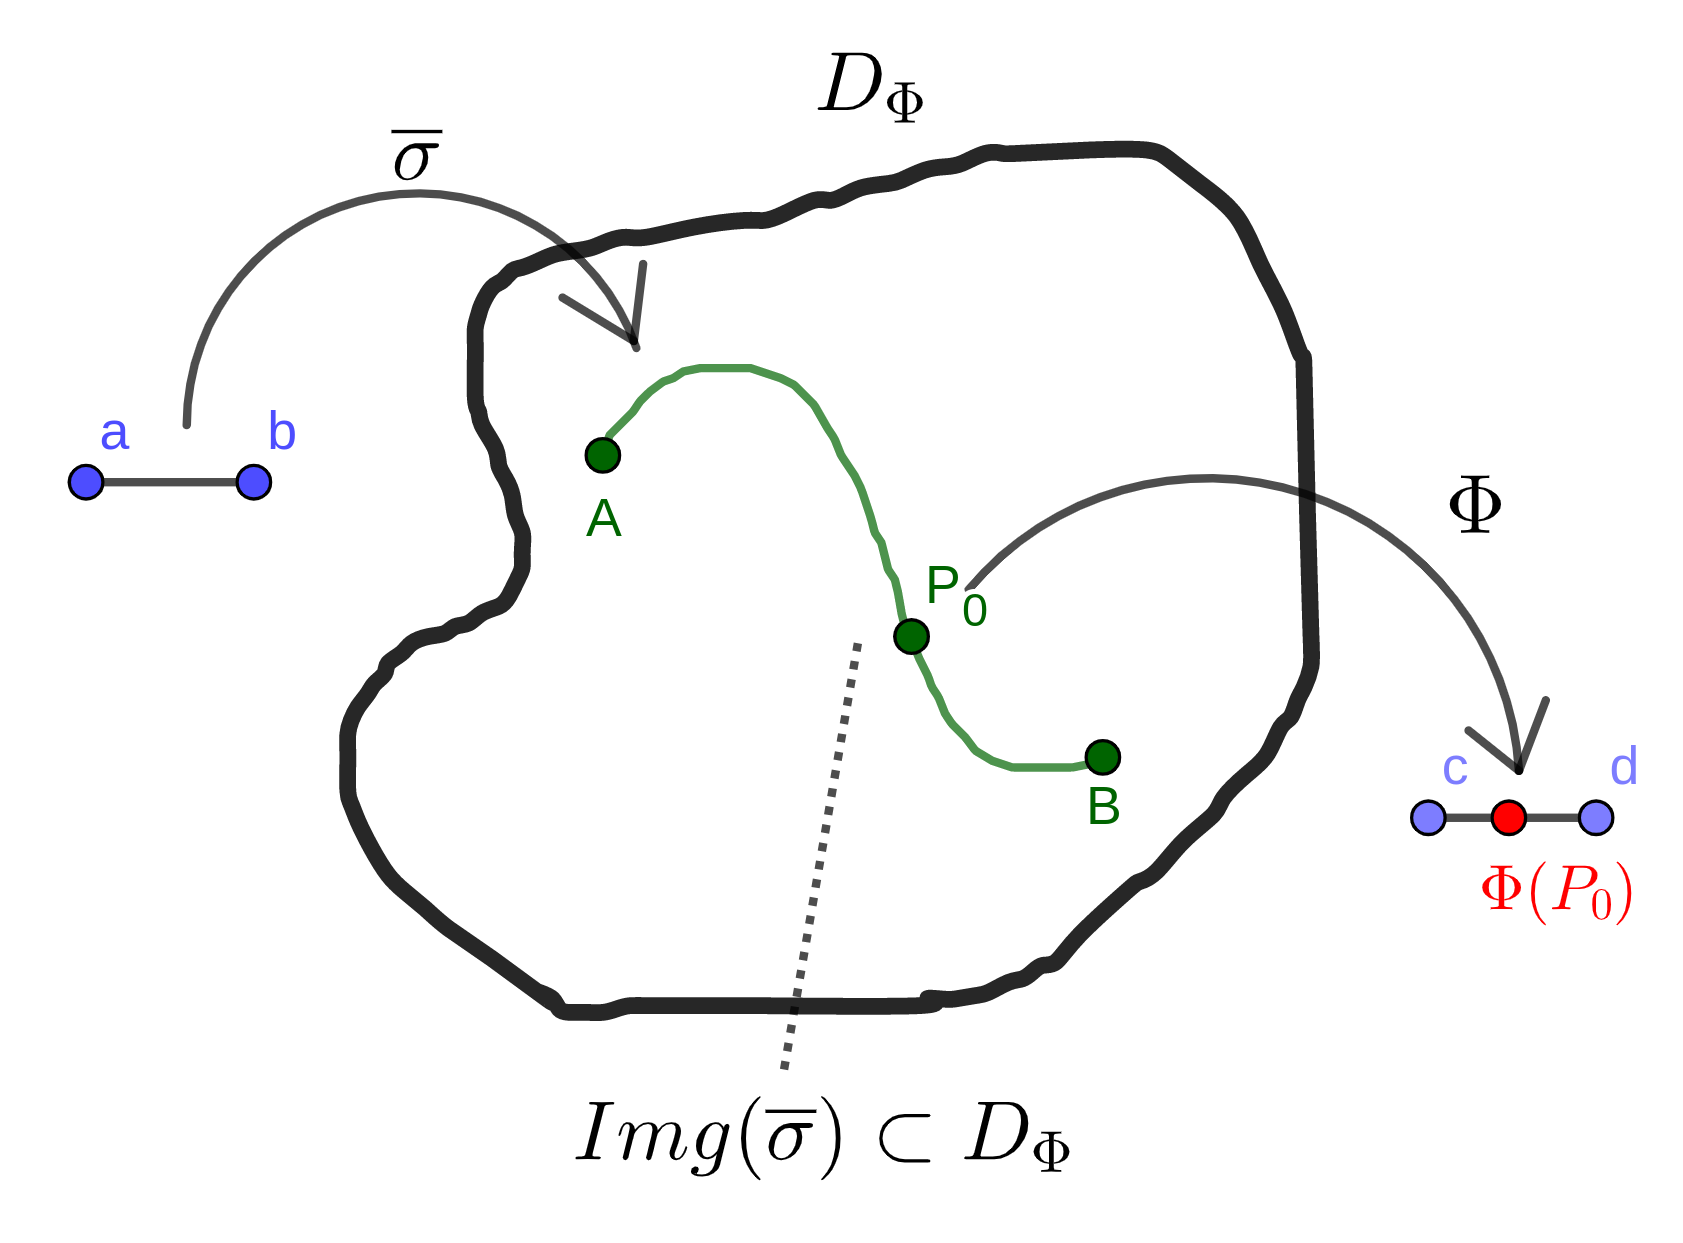
\includegraphics[scale=0.75]{img/teo_fig014_cc.png}
\end{figure}

El diferencial del campo escalar es entonces, en el punto $P_0$:

\begin{equation}
d\Phi(P_0) = \nabla\Phi(P_0) \cdot H = \Phi_{x_1}(P_0) \mathop{dx_1} + \ldots + I_{x_n}(P_0) \mathop{dx_n} 
\end{equation}

Por otro lado, considérese la integral de línea del gradiente de $\Phi$ sobre la curva $\overrightarrow{\sigma}$:

\begin{equation}
\int_{\overrightarrow{\sigma}} \overrightarrow{\nabla}\Phi \cdot d\overrightarrow{\sigma} = \int_a^b \underbrace{ \overrightarrow{\nabla}\Phi( \overrightarrow{\sigma}(t) ) \overrightarrow{\sigma}'(t) }_{d\Phi(\overrightarrow{\sigma}(t))} \mathop{dt} = \Phi(\overrightarrow{\sigma}(b)) - \Phi(\overrightarrow{\sigma}(b)) = \Phi(B) - \Phi(A)
\end{equation}

Ejemplo: Sea la curva $C$ de la figura~\ref{fig:ccej}, con punto inicial $A$ y punto final $B$. Sea el campo vectorial $\overrightarrow{f}(x,y) = (y, x)$. Planteando en términos del lema:

\begin{figure}[ht]
\centering
\caption{Ejemplo}
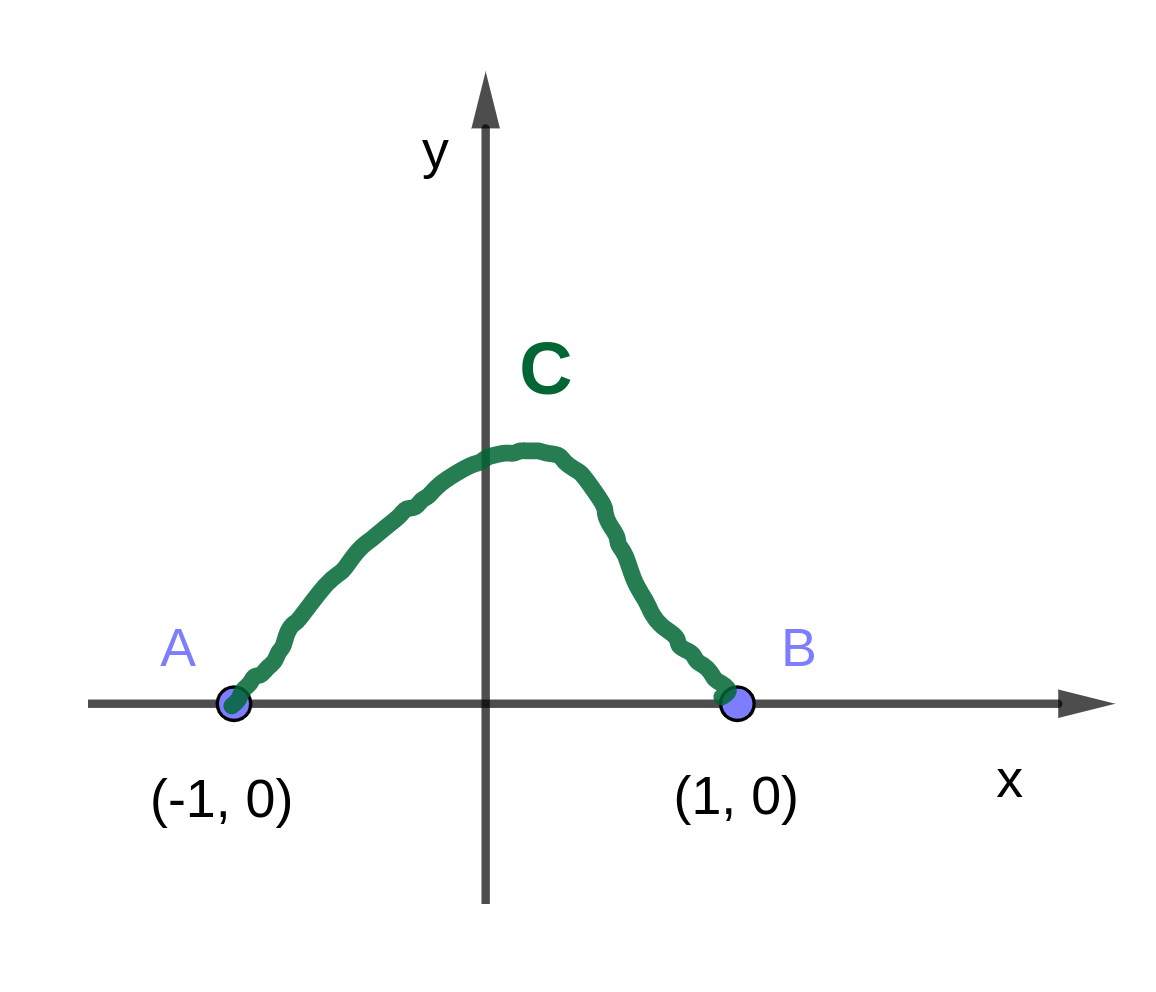
\includegraphics[scale=1]{img/teo_fig015_ccej.png}
\label{fig:ccej}
\end{figure}

\begin{equation}
\int_{\overrightarrow{\sigma}} \overrightarrow{f} d\overrightarrow{\sigma} = \int_C y \mathop{dx} + x \mathop{dy}
\end{equation}

La expresión de $\overrightarrow{\sigma}$ no interesa. Si el campo vectorial $\overrightarrow{f}$ puede expresarse como el gradiente de un campo escalar $\Phi$ a determinar, la integral puede calcularse con el resultado del lema. En este caso, por inspección:

\begin{equation}
\overrightarrow{f}(x, y) = \overrightarrow{\nabla}\Phi(x, y) = (y, x) = (\Phi_x, \Phi_y) \Rightarrow \Phi(x, y) = xy
\end{equation}

Conocido $\Phi$, la integral de línea puede calcularse evaluándolo en $A$ y $B$:

\begin{equation}
\int_C y \mathop{dx} + x \mathop{dy} = \Phi(B) - \Phi(A) = 1 \cdot 0 - (-1 \cdot 0) = 0
\end{equation}

\textbf{Definición}: Un campo vectorial es un \textbf{campo de gradientes (CG)} si y sólo si es el gradiente de un campo escalar. Simbólicamente:

\begin{equation}
\overrightarrow{f} \text{ es CG } \Leftrightarrow \exists \Phi / \overrightarrow{f} = \nabla \Phi
\end{equation}

Entonces, dada la integral de línea $\int_{\overrightarrow{\sigma}} P \mathop{dx} + Q \mathop{dy}$, resulta $\overrightarrow{f} = (P, Q)$. Para que $\overrightarrow{f}$ sea CG, necesariamente:

\begin{equation}
\nabla\Phi = \overrightarrow{f} \Rightarrow (\Phi_x, \Phi_y) = (P, Q)
\end{equation}

Derivando la última igualdad miembro a miembro en el primer componente respecto a $y$ y en el segundo componente respecto a $x$, resulta:

\begin{equation}
(\Phi_{xy}, \Phi_{yx}) = (P_y, Q_x)
\end{equation}

Nótese que esto exige que $\Phi \in C^2$ y $\overrightarrow{f} \in C^1$. Ahora bien, por el Teorema de Schwartz, siendo $\Phi \in C^2 \Rightarrow \Phi_{xy} = \Phi_{yx} \Rightarrow P_y = Q_x$. Esto establece la llamada \textbf{condición de simetría} sobre el campo $\overrightarrow{f}$: para que $f$ sea CG, sus derivadas parciales deben cumplirla. Dicha condición es necesaria: campos vectoriales que no la cumplan no son CG. Por otro lado, puede probarse que dicha condición es suficiente si $Dom f$ es un conjunto \textbf{simplemente conexo}. Vale decir, el interior de todo lazo pertenece al conjunto.

\subsection{Encontrando $\Phi$}

En el ejemplo, se pudo obtener $\Phi$ por inspección. En el caso más general, hay que resolver un sistema de ecuaciones diferenciales en derivadas parciales:

\begin{equation}
\left\{
\begin{array}{ll}
\Phi_x = P \\
\Phi_y = Q
\end{array}
\right.
\end{equation}

Un algoritmo posible:

\begin{enumerate}
\item Tomar la primera o segunda ecuación e integrarla miembro a miembro respecto a la variable del subíndice de $\Phi$. Por ejemplo, tomando la primera:

\begin{equation}
\Phi(x,y) = \text{integral de P resp. a x} + \mu(y)
\end{equation}

La función $\mu(y)$ se introduce para permitir ajuste.

\item En la otra ecuación, reemplazar para obtener $\mu(y)$, y con ello finalmente obtener $\Phi(x,y)$

\end{enumerate}

Nótese que si $\overrightarrow{f}$ es CG, la integral de línea sobre cualquier lazo contenido en su dominio es cero, y aún más importante: \textbf{la integral entre dos puntos no depende de la trayectoria}. A los campos de este tipo se los denomina \textbf{campos conservativos}.

\section{Clase T15: Integración múltiple}

\subsection{Integral doble}

Sea $R = [a, b] \times [c, d]$, un rectángulo en $\Bbb R^2$.

Sean los puntos $(x_i, y_i)$:

\begin{equation}
\left.
\begin{array}{ll}
& \Pi_x: a = x_0 < x_1 < \ldots < x_{n-1} < x_n = b \\
& \Pi_y: c = y_0 < y_1 < \ldots < y_{m-1} < y_m = d
\end{array}
\right\} \Pi = \Pi_x \times \Pi_y
\end{equation}

Sea $||\Pi|| = \max\{ \Delta x_i \Delta y_j \}$ el subrectángulo de mayor área.

Sea $P_{ij} = (\xi_i, \eta_j)$ con $x_i \leq \xi_i \leq x_{i+1}$ e $y_j \leq \eta_j \leq y_{j+1}$

Para visualizar estos objetos juntos, ver la figura~\ref{fig:intmul}.

\begin{figure}[ht]
\centering
\caption{Integración múltiple}
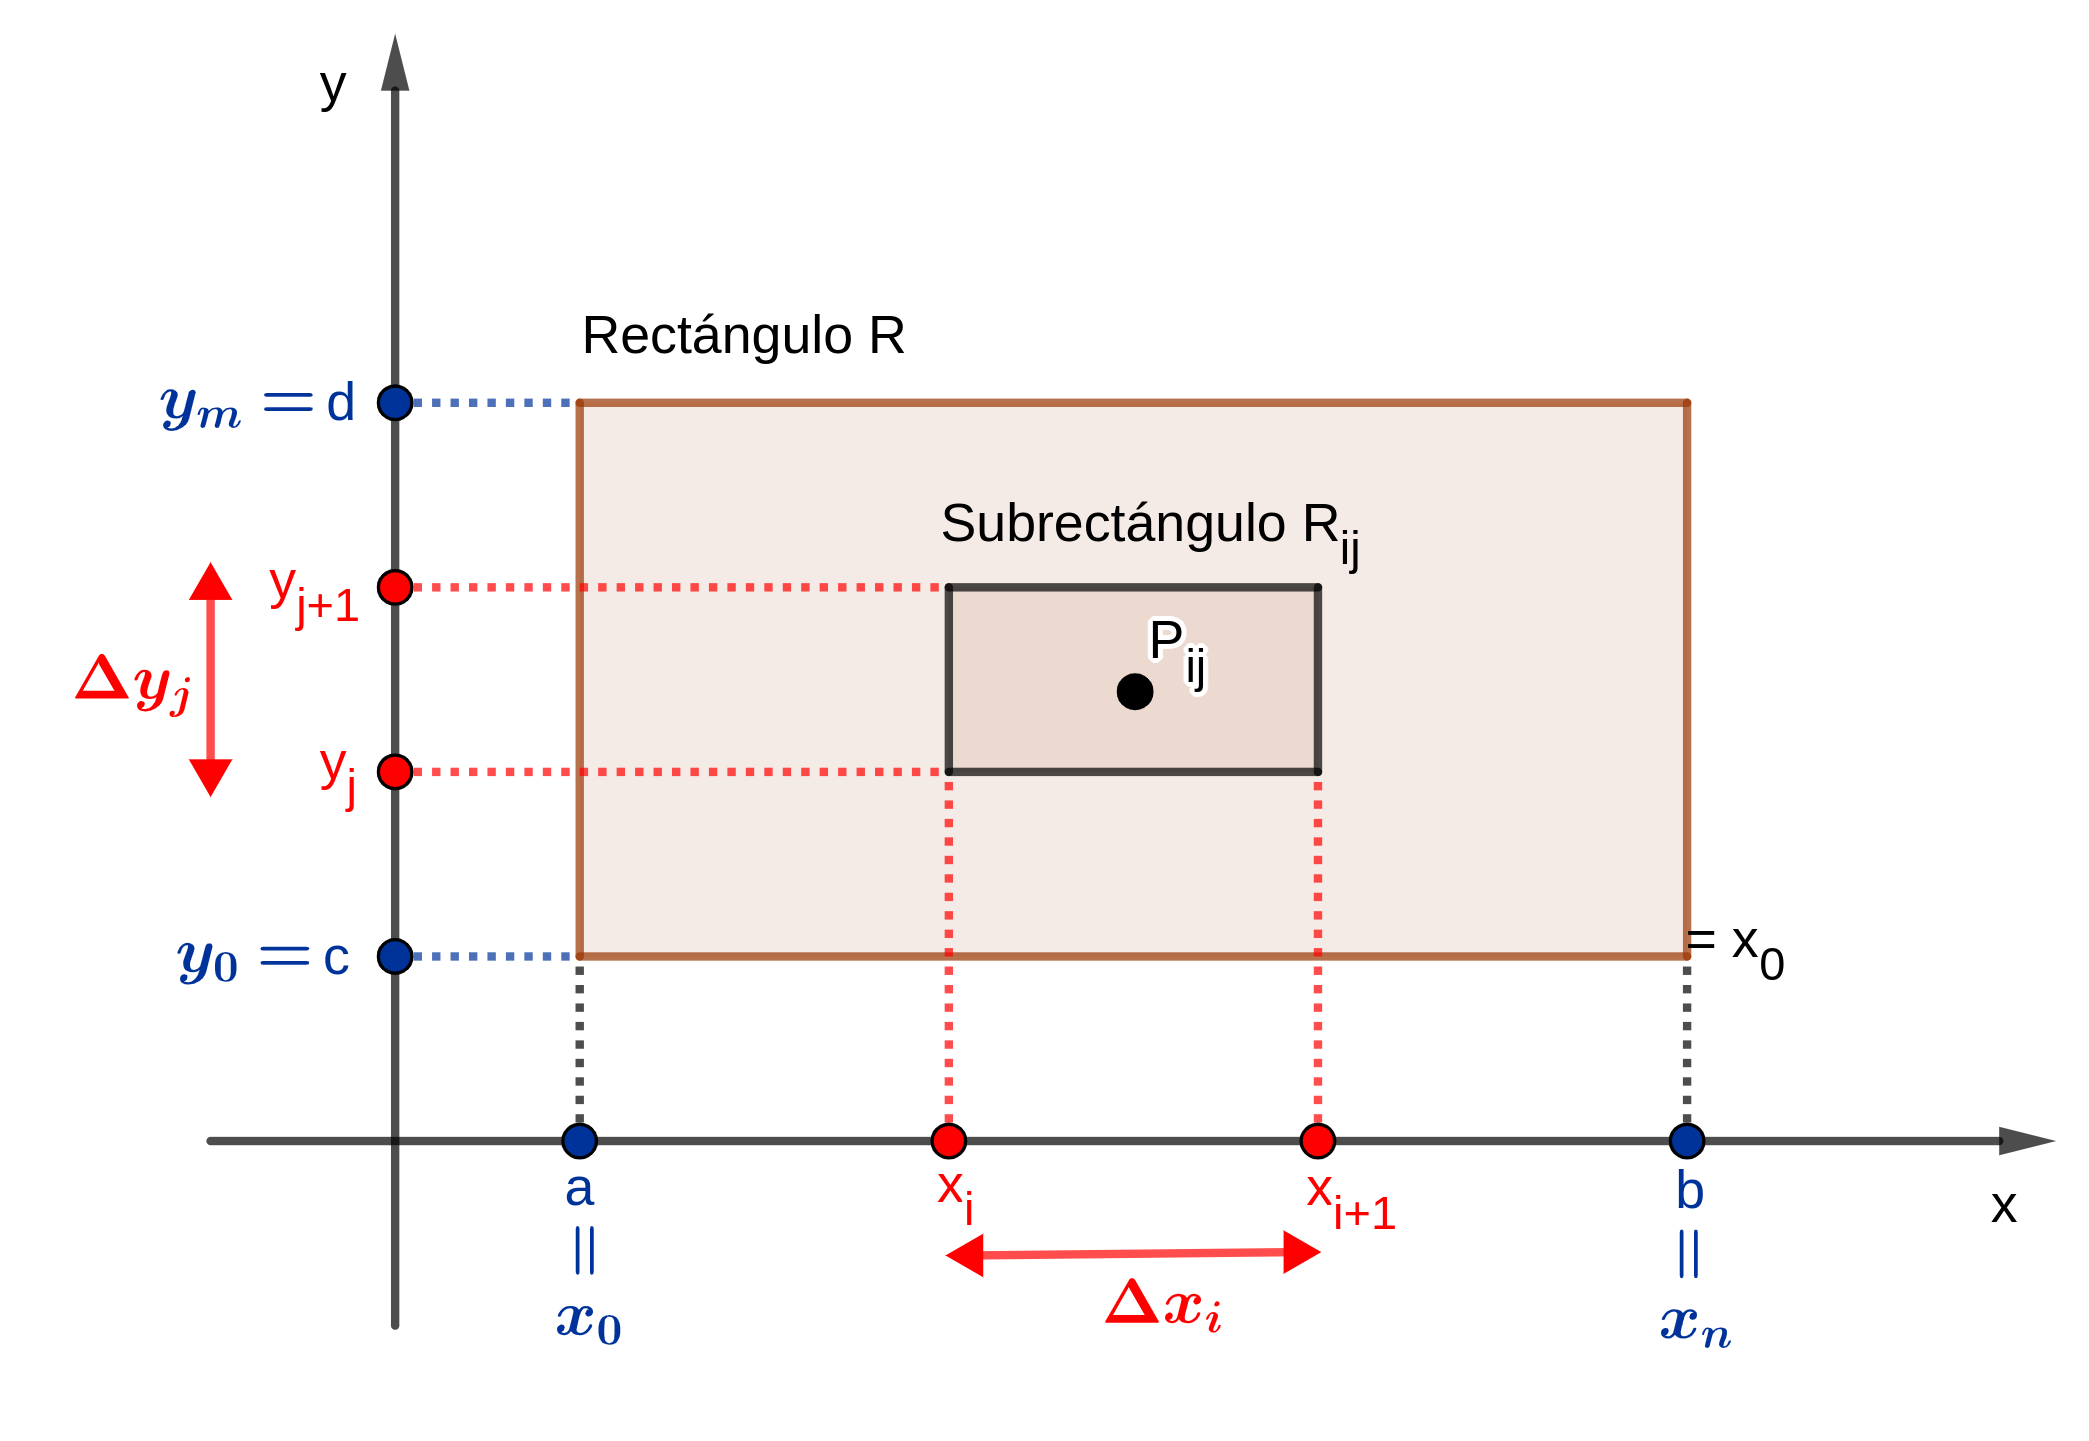
\includegraphics[scale=0.8]{img/teo_fig016_im.png}
\label{fig:intmul}
\end{figure}

A continuación, sea $f$ un campo escalar acotado en $R$, y:

\begin{align}
m_{ij} &= \inf \{ f(x,y) \text{ con } (x,y) \in R_{ij} \} \\
m &= \inf \{ f(x,y) \text{ con } (x,y) \in R \} \\
M_{ij} &= \sup \{ f(x,y) \text{ con } (x,y) \in R_{ij} \} \\
M &= \sup\{ f(x,y) \text{ con } (x,y) \in R \} \\
\end{align}

En este contexto, $\inf$ es el ínfimo, y $\sup$ el supremo; son los mínimos y máximos valores en el subrectángulo $R_{ij}$ y el rectángulo $R$, respectivamente. Con estas definiciones en mente, vale la siguiente desigualdad:

\begin{equation}
m \leq m_{ij} \leq f(P_{ij}) \leq M_{ij} \leq M
\end{equation}

Multiplicando miembro a miembro por el área del subrectángulo $R_{ij}$, o sea $\Delta x_i \Delta y_j$:

\begin{equation}
m \Delta x_i \Delta y_j \leq m_{ij} \Delta x_i \Delta y_j \leq f(P_{ij}) \Delta x_i \Delta y_j \leq M_{ij} \Delta x_i \Delta y_j \leq M \Delta x_i \Delta y_j
\label{eq:desim}
\end{equation}

Considerando todos los subrectángulos $R_{ij}$, hay $n m$ desigualdades como la de la ecuación~\ref{eq:desim}. Si se las suma a todas miembro a miembro, se obtiene:

\begin{equation}
m \underbrace{(b-a) (c-d)}_{\text{area de } R} \leq \underbrace{ s(\Pi) }_{\sum_{ij} m_{ij}} \leq \underbrace{ \sigma(\Pi) }_{\text{SUMA DE RIEMANN}} \leq \underbrace{ S(\Pi) }_{\sum_{ij} M_{ij}} \leq M \underbrace{(b-a) (d-c)}_{\text{area de } R}
\end{equation}

Cuando $n \rightarrow \infty, m \rightarrow \infty$, las sumas de ínfimos y supremos se acercan a la suma de Riemann; asumiendo que la misma es finita, $\sigma = \lim\limits_{\substack{n \rightarrow \infty \\ m \rightarrow \infty}} \sigma(\Pi)$. 

Sean:

\begin{align}
s &= \sup\{ s(\Pi) \text{ } \forall \Pi \} \\
S &= \inf\{ S(\Pi) \text{ } \forall \Pi \}
\end{align}

Si $f$ es tal que $s = \sigma = S$, $f$ es integrable en $R$, y $\sigma$ es la \textbf{integral doble} de $f$ sobre $R$:

\begin{equation}
\iint_R f(x,y) \mathop{dx} \mathop{dy} = s = S = \sigma
\end{equation}

A partir de este análisis, puede demostrarse que:

\begin{equation}
\tcboxmath[colback=orange!25!white,colframe=orange]
{ \text{Si } f \text{ es continua en } R \text{, es integrable en } R }
\end{equation}

Observaciones:

\begin{enumerate}[(A)]
\item Si $f(x,y) = 1 \Rightarrow \iint_R \mathop{dx} \mathop{dy} = $ área del rectángulo $R$. 
\item Si $f(x,y) \geq 0$ en $R$, la integral doble da como resultado el volumen del sólido limitado por $R$ y la superficie $z= f(x,y)$. Por ejemplo, considerando la figura~\ref{fig:volbajosup}, dada la superficie $z=f(x,y)$ (color rosa), el volumen delimitado entre $R$ en el plano $(x,y)$ y dicha superficie corresponde al sólido delimitado con colores verdes.

\begin{figure}[ht]
\centering
\caption{Volumen bajo superficie}
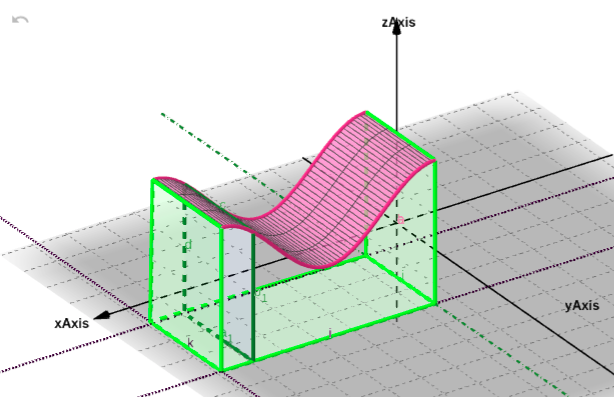
\includegraphics[scale=0.75]{img/teo_fig017_vbs.png}
\label{fig:volbajosup}
\end{figure}

Denominando $K$ a dicho sólido,

\begin{align}
K &= \{ (x,y,z) \in \Bbb R^3 / (x,y) \in R \wedge 0 \leq z \leq f(x,y) \} \\
vol(K) &= \iint_{R} f(x,y) \mathop{dx} \mathop{dy}
\end{align}

\item \textbf{Teorema de Fubbini}: Si $f$ es continua en $R$ exceptuando al conjunto de medida/contenido nulo,

\begin{equation}
\tcboxmath[colback=orange!25!white,colframe=orange, title=Teorema de Fubbini]
{
\begin{array}{ll}
\iint_R f(x,y) \mathop{dx} \mathop{dy} = \int_a^b \left( \int_c^d f(x,y) \mathop{dy} \right) \mathop{dx} \\
\iint_R f(x,y) \mathop{dx} \mathop{dy} = \int_c^d \left( \int_a^b f(x,y) \mathop{dx} \right) \mathop{dy}
\end{array}
}
\end{equation}

Lo que este teorema dice es que dadas sus condiciones, la integral doble puede resolverse integrando primero respecto a $x$ y luego $y$, o viceversa. El resultado debería ser el mismo.

¿Qué se entiende por \textbf{conjunto de contenido nulo}? En $\Bbb R^2$, es un recinto de área nula. En $\Bbb R$, un segmento de longitud nula. En $\Bbb R^3$, volumen nulo. Para mayores dimensiones, será un concepto extendido de tamaño de un recinto.

\item Para recintos no rectangulares, la integral doble puede calcularse según el tipo de recinto.

\begin{enumerate}
\item Dos lados verticales paralelos. Véase la figura~\ref{fig:d1}.

\begin{figure}[ht]
\centering
\caption{Recinto con dos lados verticales paralelos}
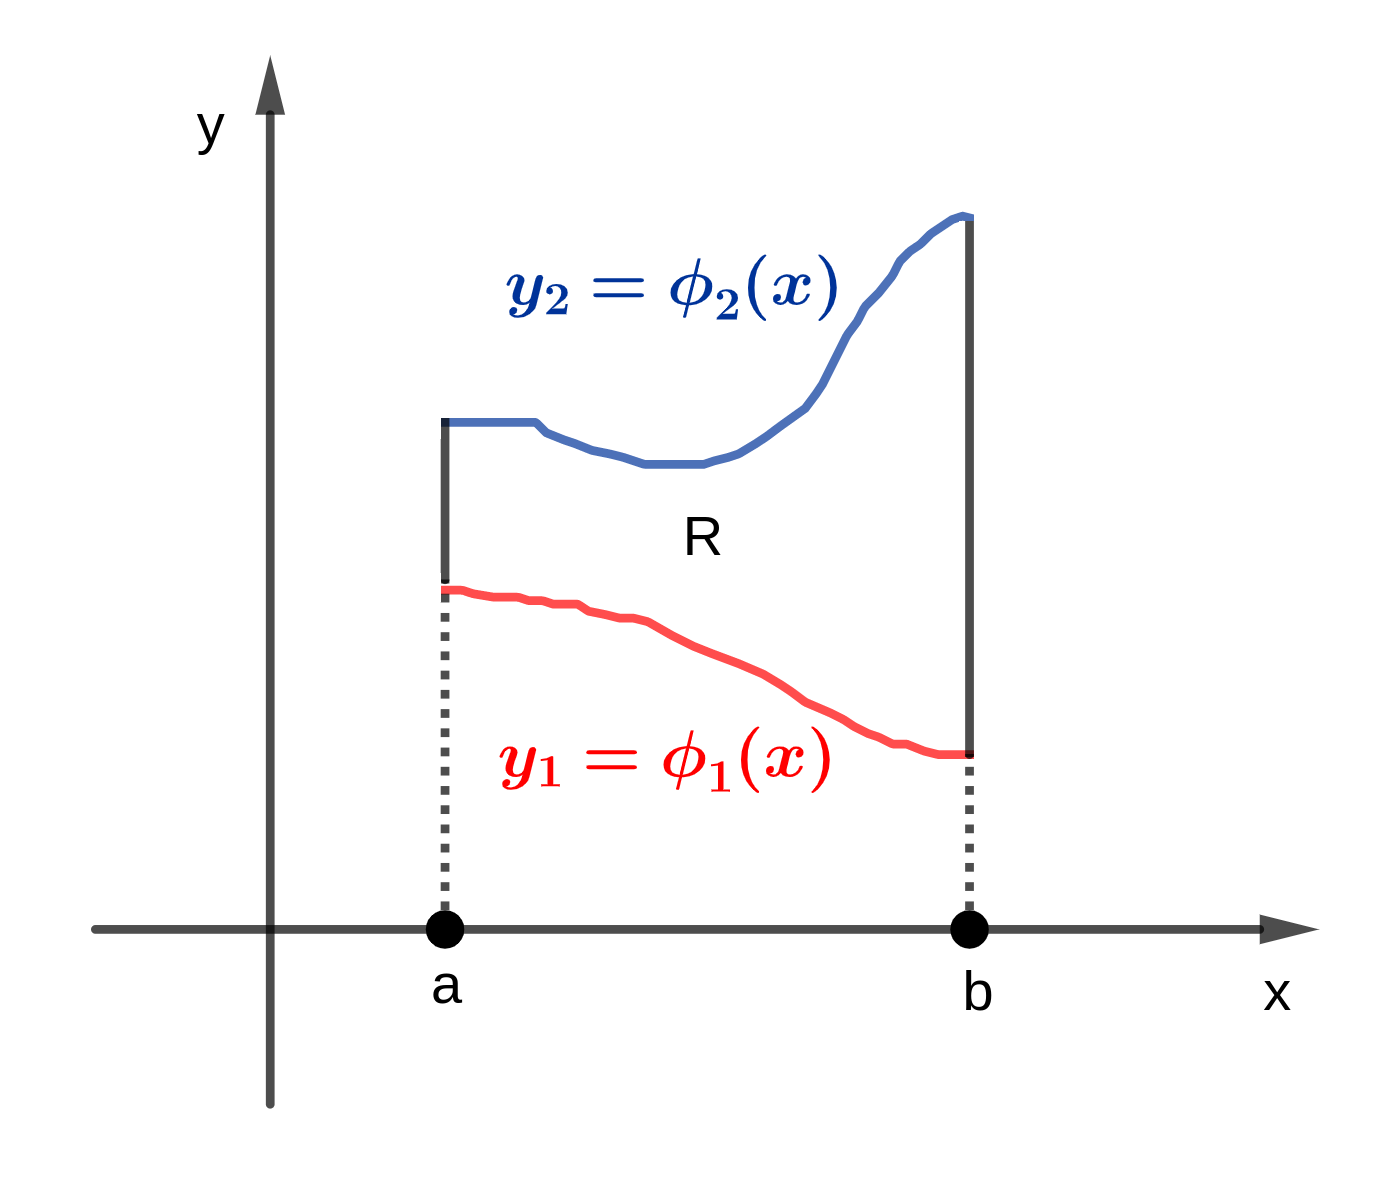
\includegraphics[scale=0.75]{img/teo_fig018_d1.png}
\label{fig:d1}
\end{figure}

\begin{align}
\iint_R f(x,y) \mathop{dx} \mathop{dy} &= \int_a^b \left( \int_{\phi_1(x)}^{\phi_2(x)} f(x,y) \mathop{dy} \right) \mathop{dx} \\
area(R) &= \int_a^b \left( \int_{\phi_1(x)}^{\phi_2(x)} \mathop{dy} \right) \mathop{dx}
\end{align}

\item Dos lados horizontales paralelos. Véase la figura~\ref{fig:d2}.

\begin{figure}[ht]
\centering
\caption{Recinto con dos lados horizontales paralelos}
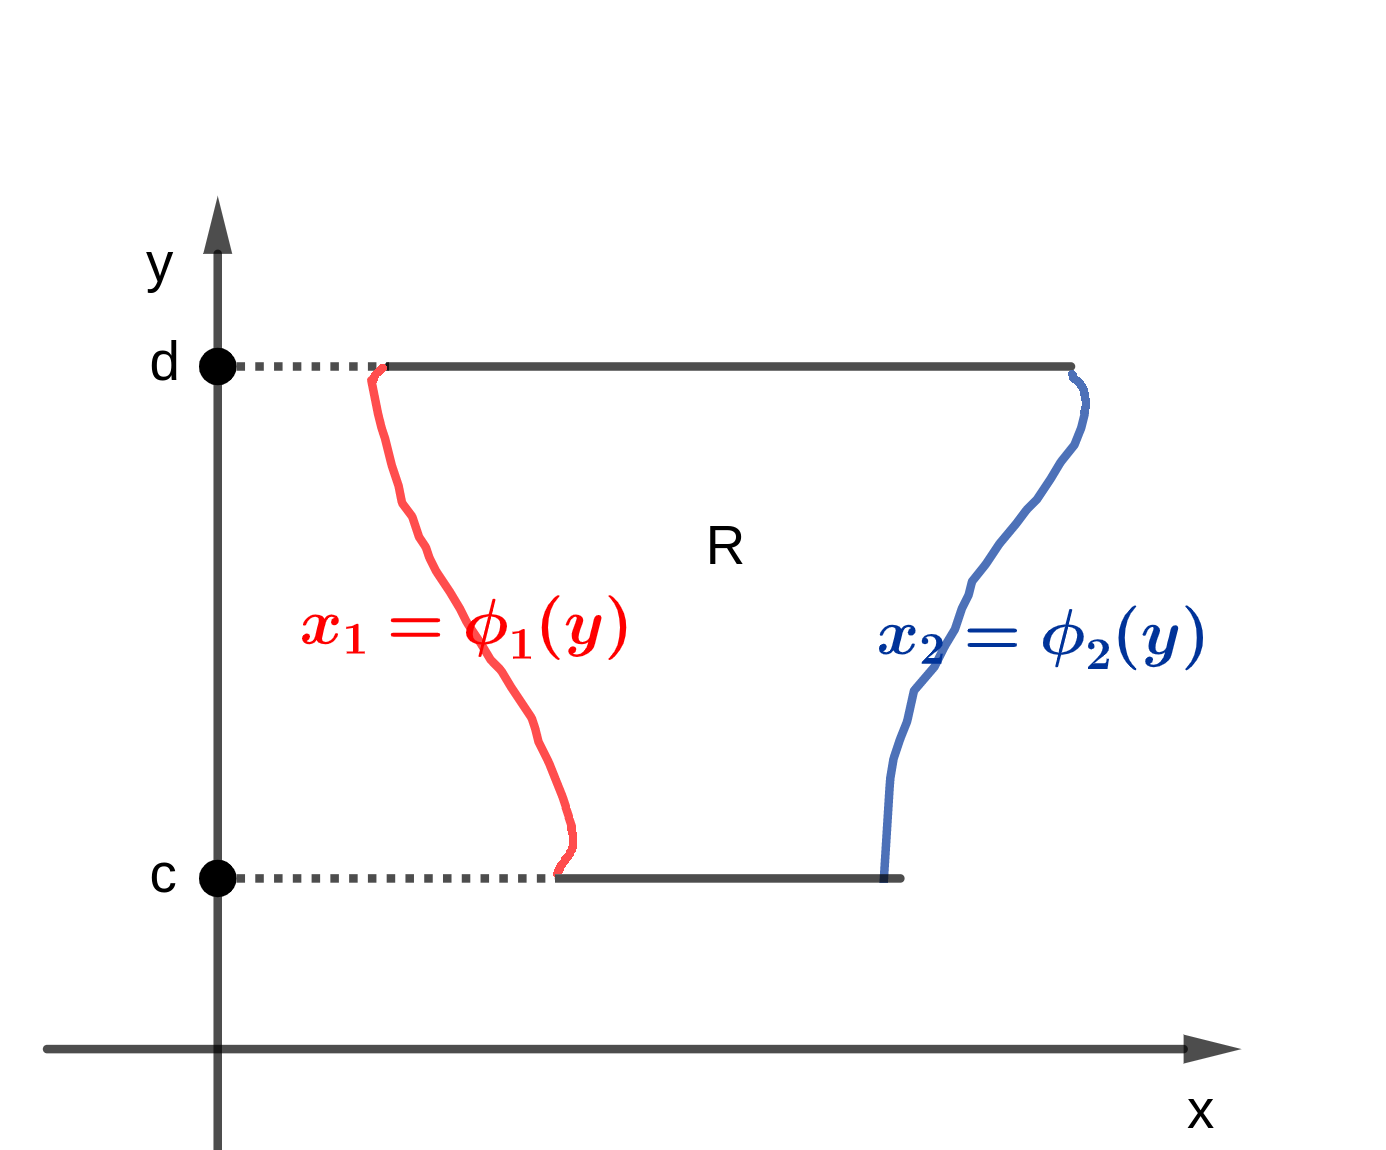
\includegraphics[scale=0.75]{img/teo_fig019_d2.png}
\label{fig:d2}
\end{figure}

\begin{align}
\iint_R f(x,y) \mathop{dx} \mathop{dy} &= \int_c^d \left( \int_{\phi_1(y)}^{\phi_2(y)} f(x,y) \mathop{dx} \right) \mathop{dy} \\
area(R) &= \int_c^d \left( \int_{\phi_1(y)}^{\phi_2(y)} \mathop{dx} \right) \mathop{dy}
\end{align}

\item 1 lado horizontal y 1 lado vertical: Puede tratarse como el caso a, o el caso b.
\end{enumerate}

\item Cambio de orden de integración

Por ejemplo, considérese la siguiente integral doble:

\begin{equation}
\int_{-5}^0 \left( \int_{-1-y^2}^{y^2} f(x,y) \mathop{dx} \right) \mathop{dy}
\end{equation}

Analizando los bordes del recinto:

\begin{align}
x = -1-y^2 &\Rightarrow y = -5 \Rightarrow x = -26 \wedge y = 0 \Rightarrow x = -1 \\
x = y^2 &\Rightarrow y = -5 \Rightarrow x =25 \wedge y = 0 \Rightarrow x = 0
\end{align}

Para invertir el orden de integración, hay que expresar las curvas que lo limitan como funciones de $x$ (ya que originalmente fueron definidas como funciones de $y$).

\begin{align}
x &= -1-y^2 \Rightarrow -x - 1 = y^2 \Rightarrow \sqrt{-x-1} = \pm y \\
x &= y^2 \Rightarrow \sqrt{x} = \pm y
\end{align}

Para saber si tomar la rama positiva o negativa de las funciones raíz cuadrada, considérese que $y$ toma los valores $-5$ y $0$. Por lo tanto, se toma la rama negativa en ambos casos. Graficar el recinto ayuda; ver la figura~\ref{fig:coi}.

\begin{figure}[ht]
\centering
\caption{Cambio de orden de integración}
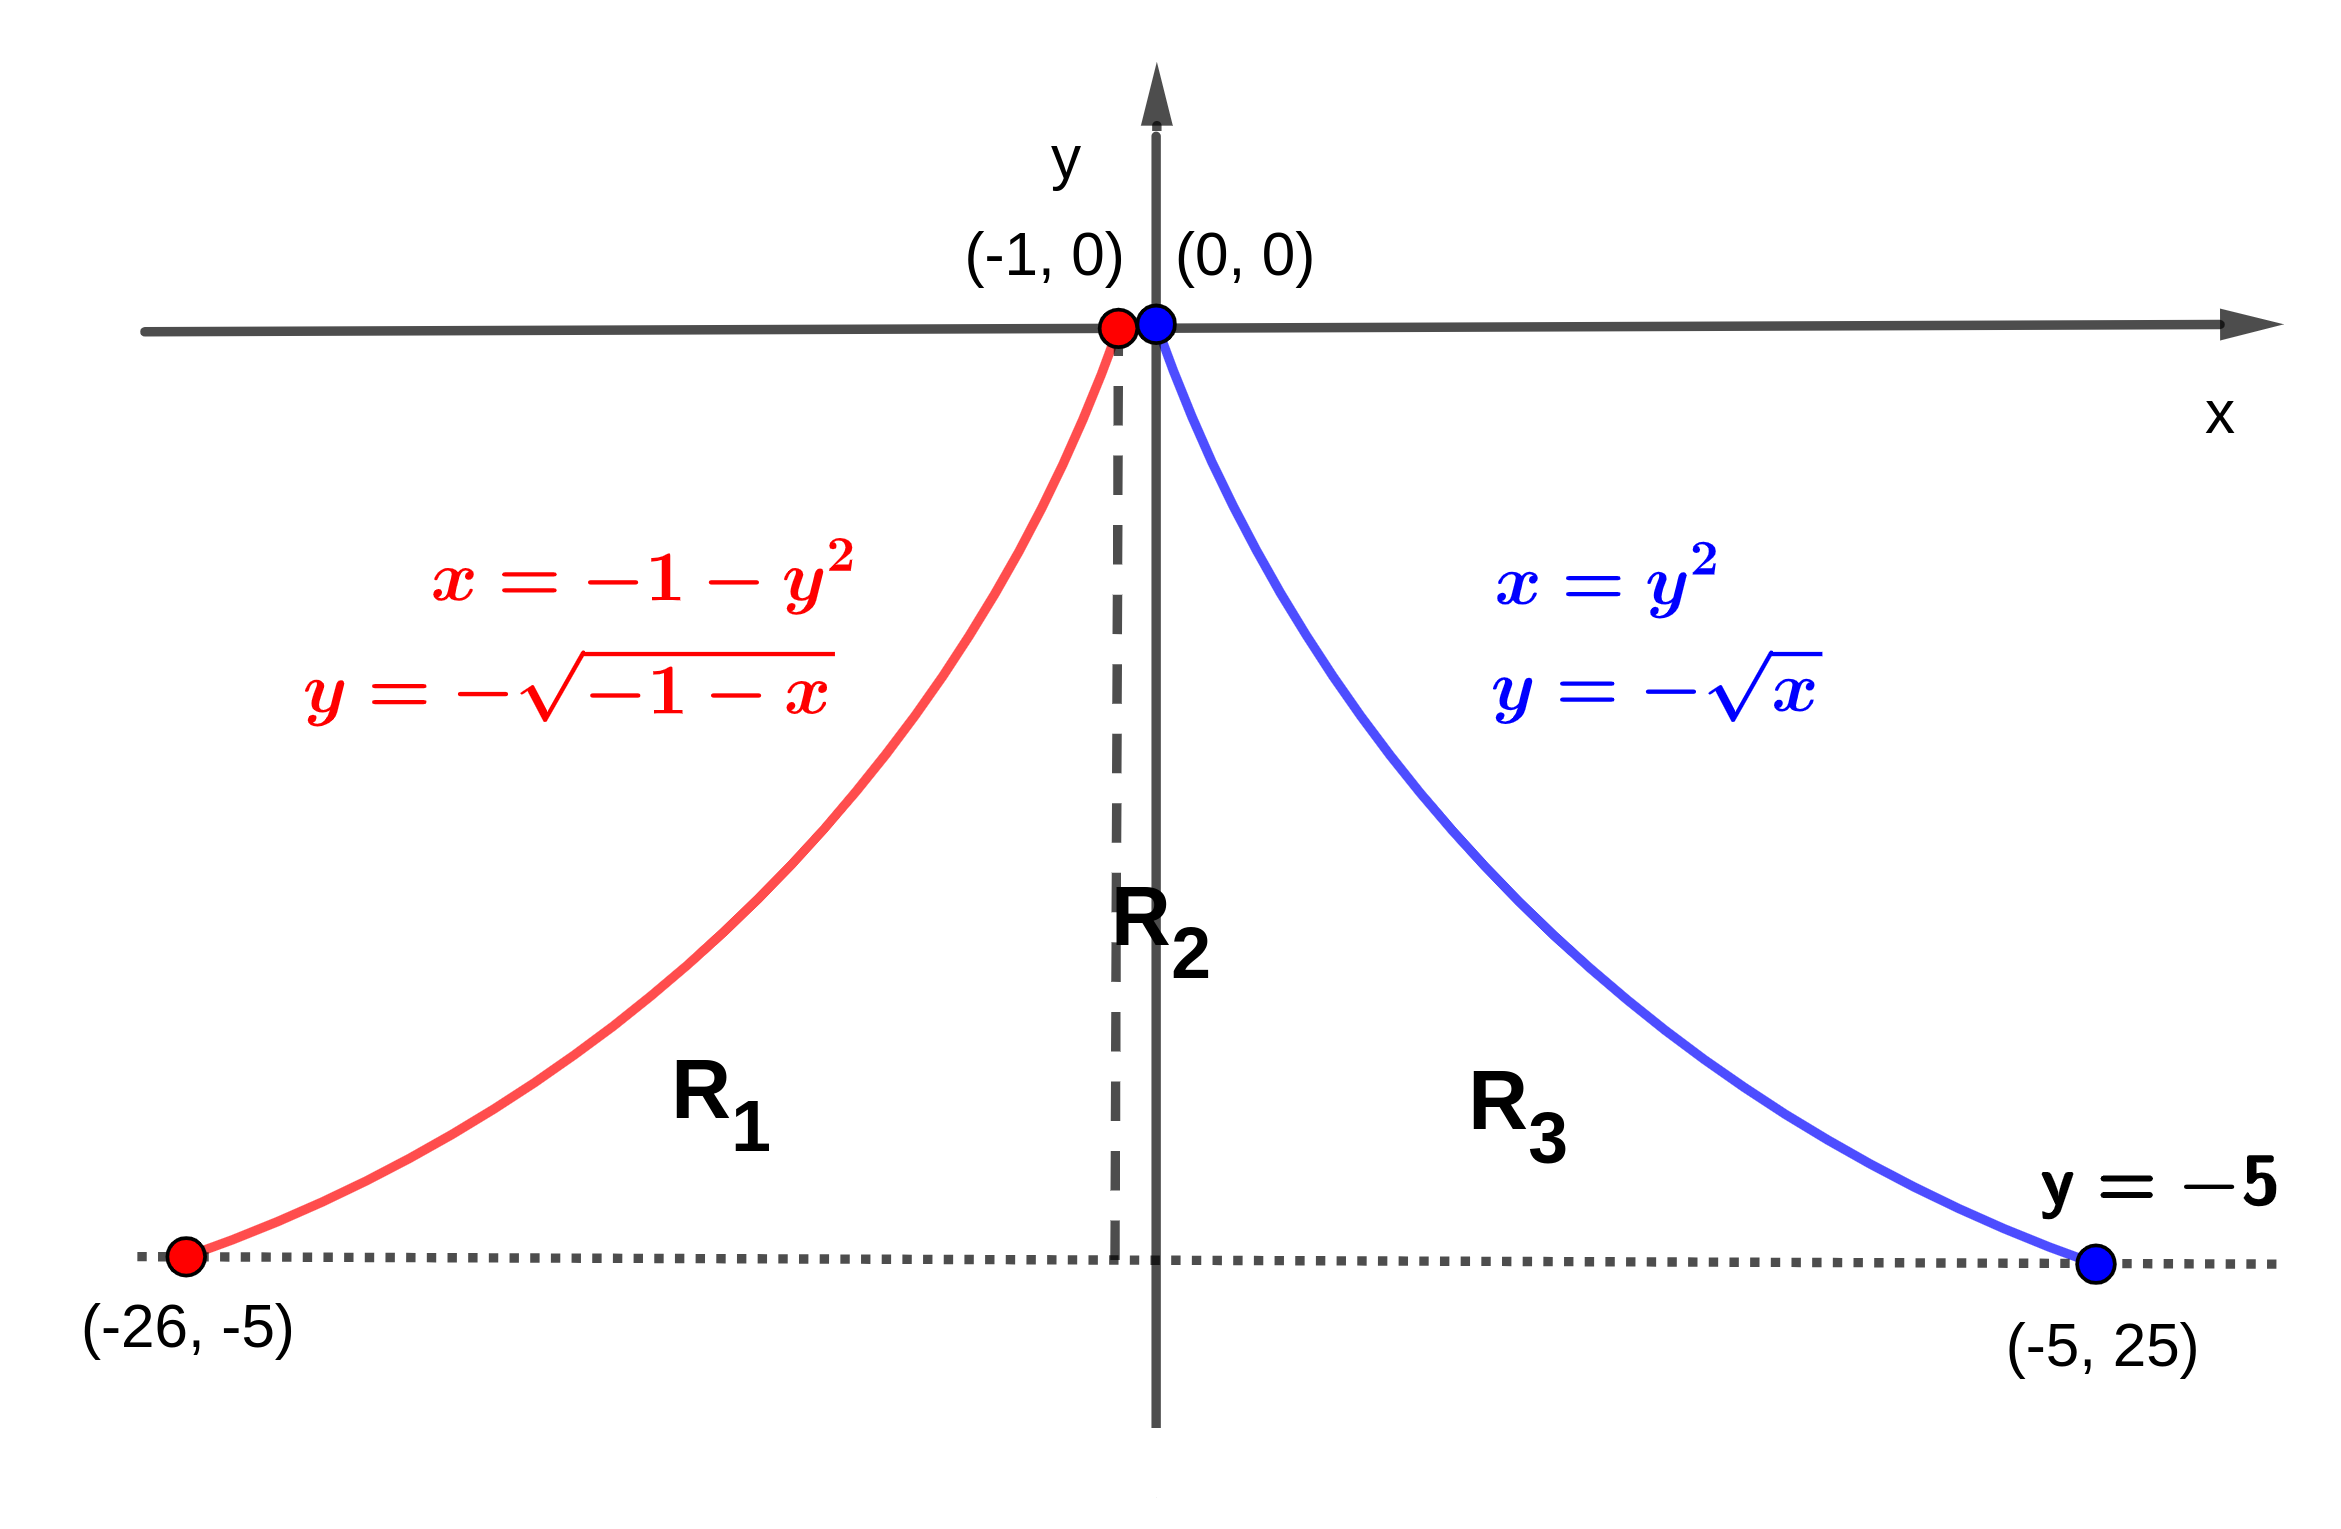
\includegraphics[scale=0.75]{img/teo_fig020_coi.png}
\label{fig:coi}
\end{figure}

Para integrar primero respecto a $y$, conviene dividir el recinto en 3 recintos $R_1, R_2$ y $R_3$ (marcados en la figura~\ref{fig:coi}), y aplicar la propiedad de linealidad de la integral, que es trivial demostrar que sigue valiendo para la integral doble. Resulta entonces:

\begin{align}
\int_{-5}^0 \left( f(x,y) \mathop{dx} \right) \mathop{dy} &= \iint_{R_1} (f(x,y) \mathop{dy}) \mathop{dx} + \iint_{R_2} (f(x,y) \mathop{dy}) \mathop{dx} + \iint_{R_3} (f(x,y) \mathop{dy}) \mathop{dx} \\
\iint_{R_1} (f(x,y) \mathop{dy}) \mathop{dx} &= \int_{-26}^{-1} \left( \int_{-5}^{-\sqrt{-1-x}} f(x,y) \mathop{dy}  \right) \mathop{dx} \\
\iint_{R_2} (f(x,y) \mathop{dy}) \mathop{dx} &= \int_{-1}^{0} \left( \int_{-5}^0 f(x,y) \mathop{dy} \right) \mathop{dx} \\
\iint_{R_3} (f(x,y) \mathop{dy}) \mathop{dx} &= \int_{0}^{25} \left( \int_{-5}^{-\sqrt{x}} f(x,y) \mathop{dy} \right) \mathop{dx}
\end{align}

\end{enumerate}

\subsection{Integral triple}

Es posible generalizar los conceptos de la integral doble partiendo de un recinto $R = [a,b] \times [c,d] \times [e,f]$, que consiste en un paralelepípedo en $\Bbb R^3$. Definiendo la integral triple sobre $R$ como $\iiint_R f(x,y,z) \mathop{dx} \mathop{dy} \mathop{dz}$, puede probarse que todos los resultados de la integral doble siguen valiendo: Fubbini, linealidad, etc.

Si $f(x,y,z) = 1$, $vol(R) = \iiint_R \mathop{dx} \mathop{dy} \mathop{dz}$

Tal como ocurría en el caso de dos dimensiones, la integral triple puede extenderse a recintos tridimensionales que no sean paralelepípedos. Por ende, la integral triple es una gran herramienta para calcular volúmenes.

Por ejemplo, sea el recinto $R$ en $\Bbb R^3$ delimitado por:

\begin{equation}
R = \{ (x,y,z) \in \Bbb R^3 / 0 \leq x \leq 1 \wedge 0 \leq y \leq 1 \wedge z = x^2 \}
\end{equation}

Gráficamente, R sería el volumen entre la superficie $z = x^2$ y el plano $(x, y)$. En la figura~\ref{fig:itv} se puede visualizar la superficie en el plano $\Bbb R^3$.

\begin{figure}[ht]
\centering
\caption{Integral triple}
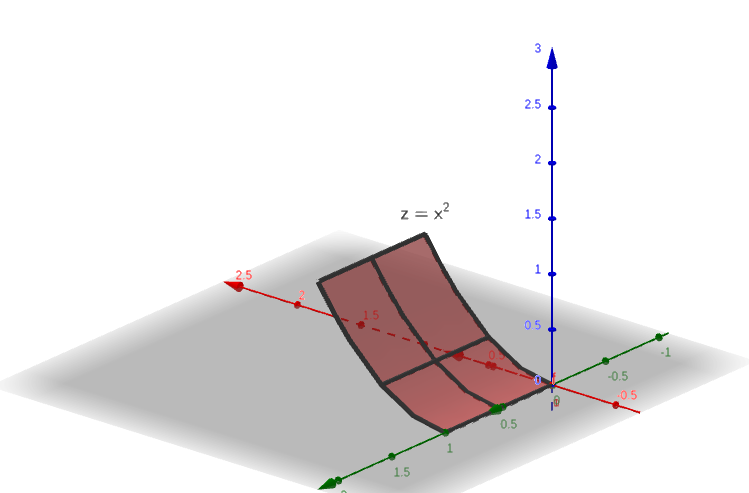
\includegraphics[scale=0.6]{img/teo_fig021_itv.png}
\label{fig:itv}
\end{figure}

Sea, arbitrariamente, $f(x,y,z) = xyz^2$:

\begin{equation}
\iiint_R f(x,y,z) \mathop{dx} \mathop{dy} \mathop{dz} = \int_0^1 \left( \int_0^1 \left( \int_0^{x^2} xyz^2 \mathop{dz} \right)  \right) \mathop{dy}) dx
\end{equation}

¿Qué representaría la integral triple de la función $f$ sobre el sólido $R$? Por ejemplo, si $f$ describiera la densidad punto a punto del sólido, la integral triple daría la masa.

\section{Clase T16}

\subsection{Coordenadas polares}

Un vector en el plano $\Bbb R^2$ puede expresarse en términos de las dos distancias $(x,y)$ a los respectivos ejes. Esta representación se conoce como coordenadas rectangulares o cartesianas y es la más usual. Alternativamente, el mismo vector puede representarse en términos del ángulo $\theta$ respecto al eje $x$, y la distancia $r$ desde el origen. El par $(r, \theta)$ son las coordenadas polares del vector.

\begin{figure}[ht]
\centering
\caption{Coordenas cartesianas y polares}
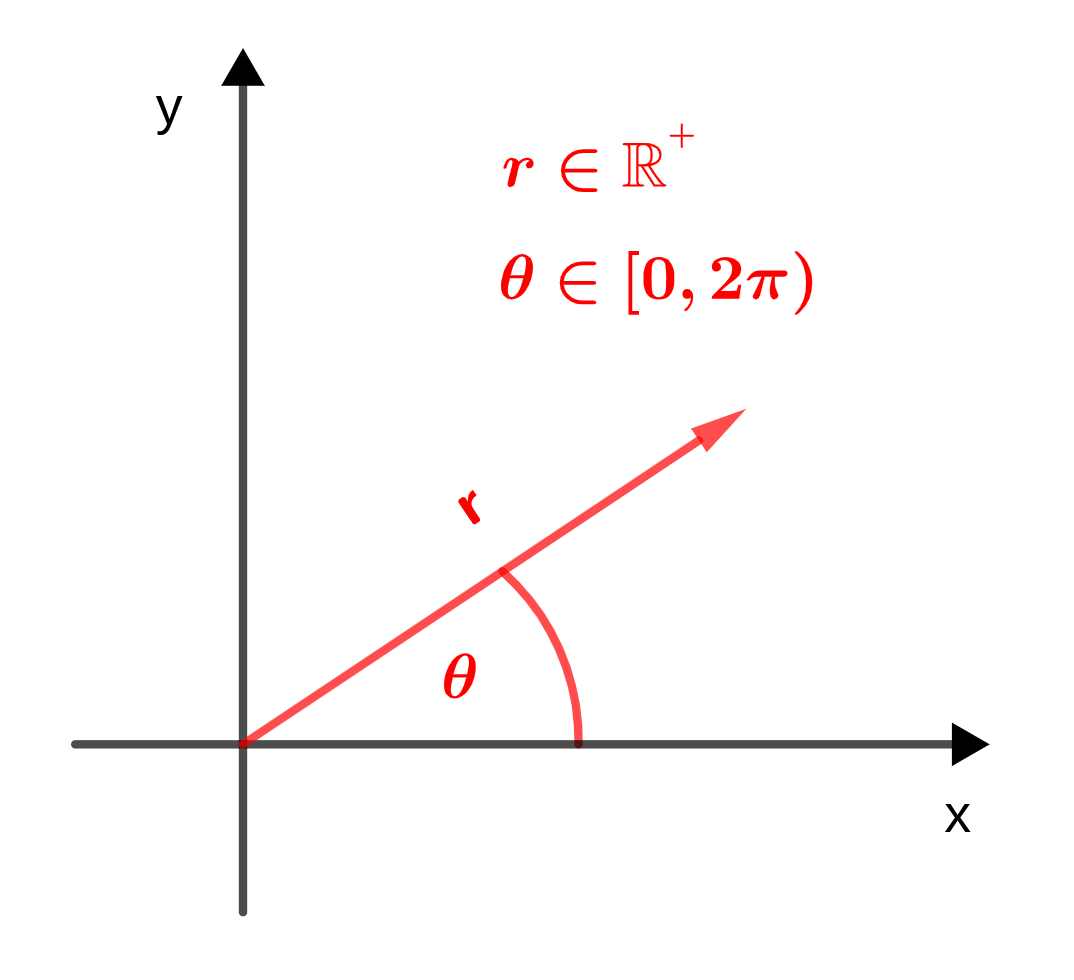
\includegraphics[scale=0.8]{img/teo_fig022_cp.png}
\label{fig:cp}
\end{figure}

La conversión de cartesianas a polares es:

\begin{equation}
(r, \theta) = \left( \sqrt{x^2 + y^2}, \arctan \left( \frac{y}{x} \right) \right)
\label{eq:cartapol}
\end{equation}

Dado el plano $(x,y)$ en coordenadas rectangulares/cartesianas, el mismo puede ser mapeado al plano $(r, \theta)$ a través de un campo vectorial $T:\Bbb R^2 \rightarrow \Bbb R^2$ como el de la ecuación~\ref{eq:cartapol}.

\begin{figure}[ht]
\centering
\caption{De polares a cartesianas}
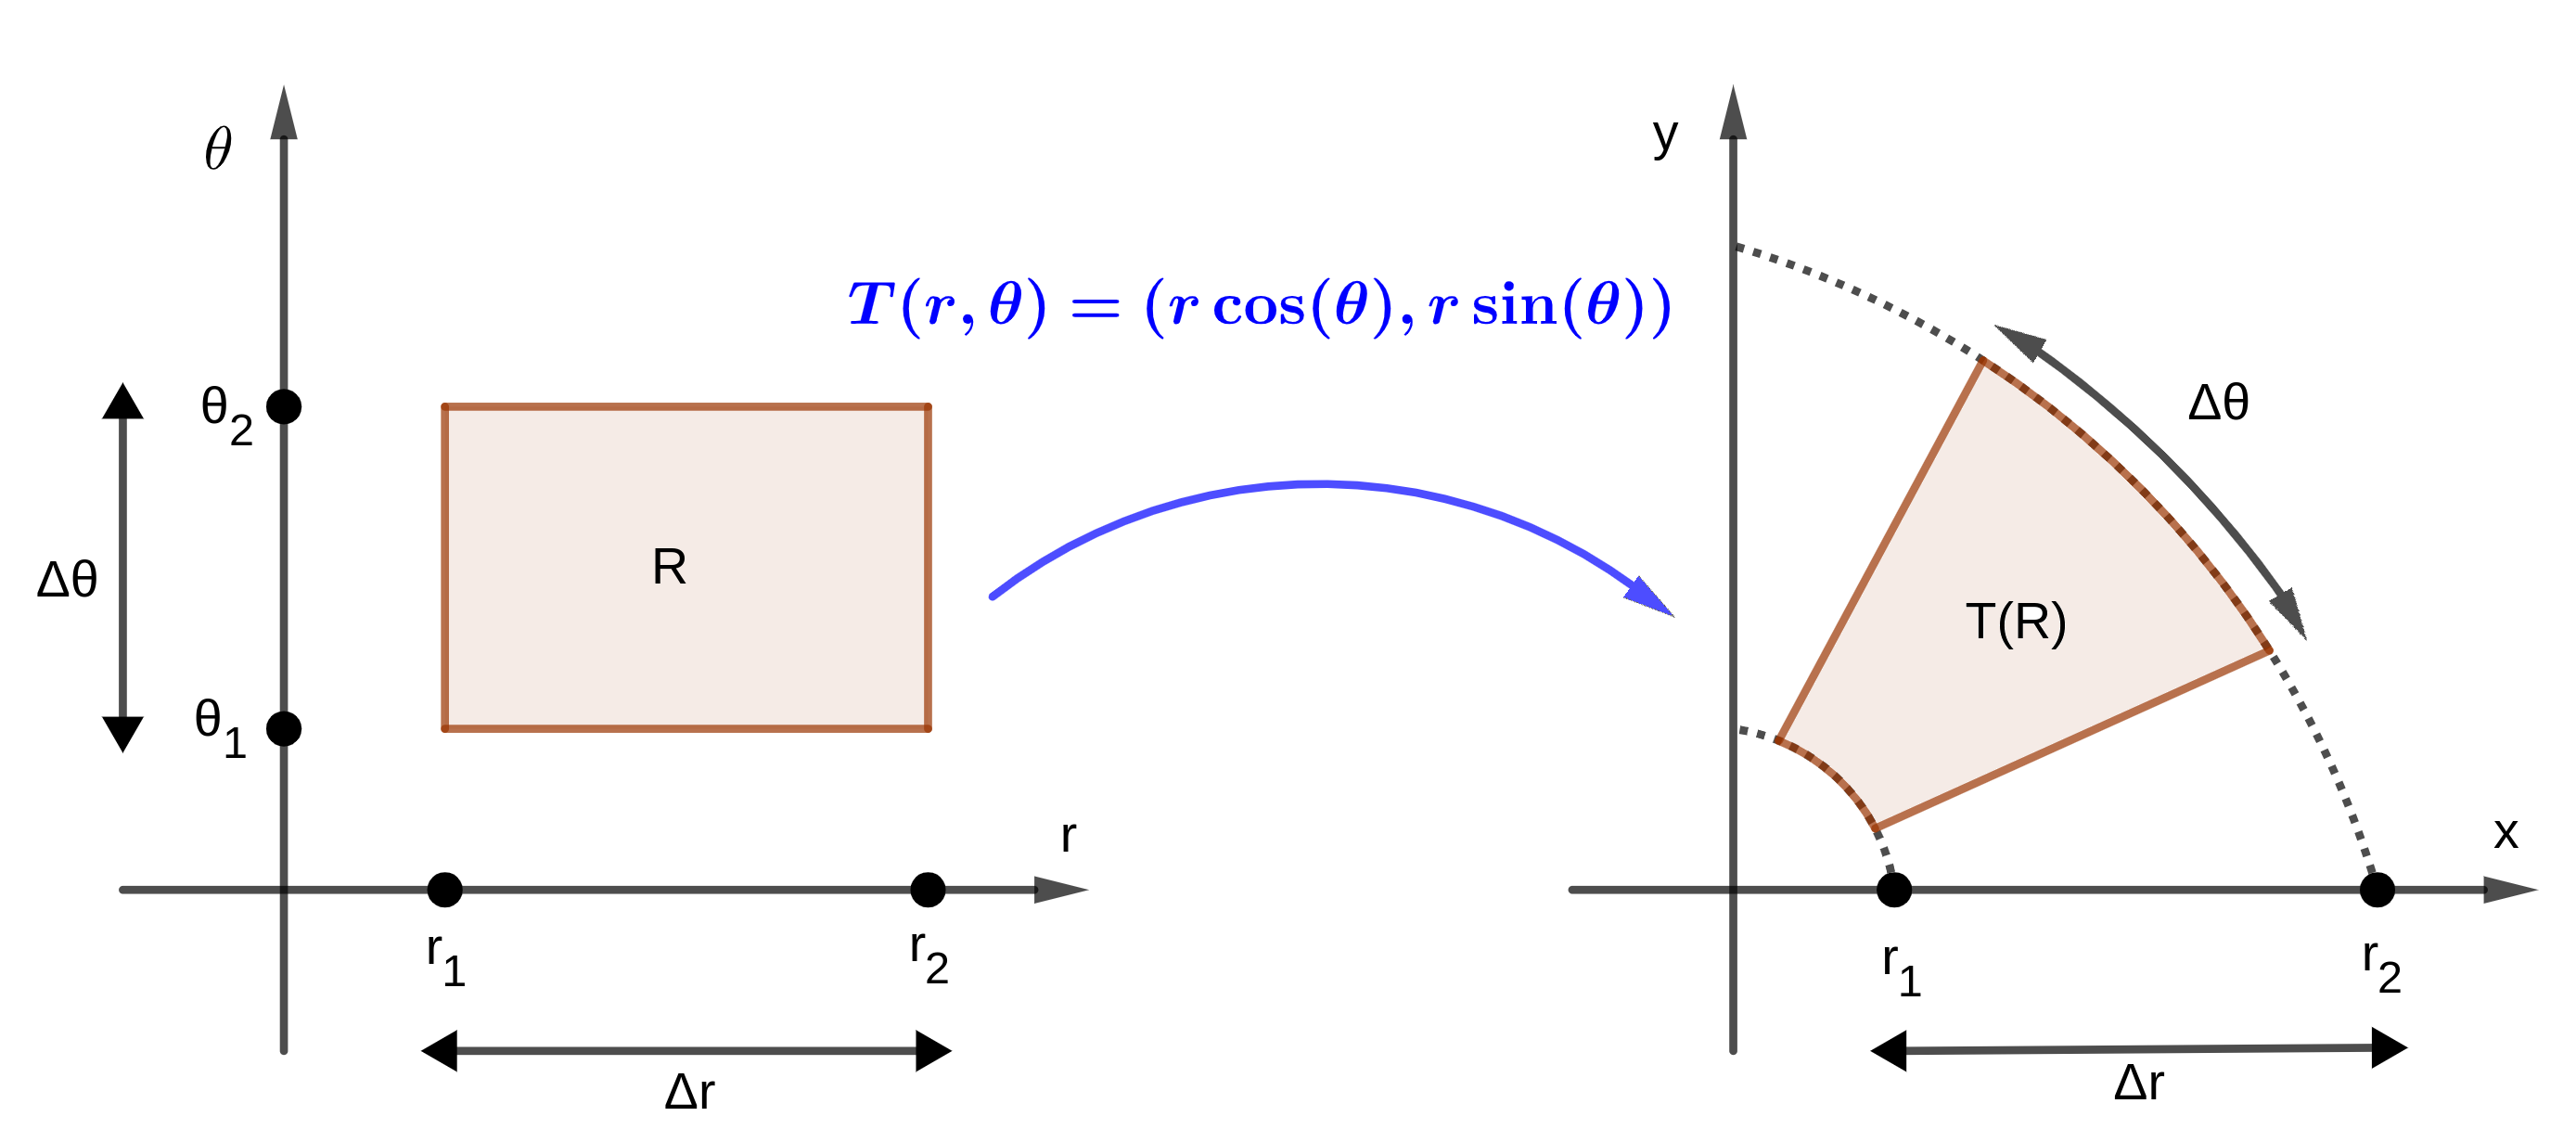
\includegraphics[scale=0.8]{img/teo_fig023_ccp.png}
\label{fig:polacart}
\end{figure}

La transformación inversa, del plano $(r, \theta)$ al plano $(x,y)$, sería como en la figura~\ref{fig:polacart}. Nótese cómo un rectángulo en coordenadas polares es transformado a un sector concéntrico de círculo. Analizando las áreas de ambas figuras (recordando que el área de un sector circular-una porción de pizza completa- es $ \frac{ \mathop{radio}^2 \mathop{longarco} }{2} $):

\begin{align}
\mathop{area}(R) &= \Delta r \Delta \theta \\
\mathop{area}(T(R)) &= \frac{r_2^2 \Delta \theta}{2} - \frac{r_1^2 \Delta \theta}{2} = \frac{(r_2^2 - r_1^2) \Delta \theta}{2} = \underbrace{ \frac{r_2 + r_1}{2} }_{\overline{r}, \text{ promedio}} \underbrace{ (r_2 - r_1) }_{\Delta r} \Delta \theta \\
\mathop{area}(T(R)) &= \overline{r} \Delta r \Delta \theta
\end{align}

Sea $T$ la transformación de coordenadas polares a cartesianas de la figura~\ref{fig:polacart}, y sea $R$ un compacto (conjunto cerrado y acotado) en el plano $(r,\theta)$. Sea $f$ un campo escalar continuo y acotado sobre el interior de R. Entonces, pensando en el cambio de coordenadas como una composición de funciones, aplicar la regla de la cadena genera la siguiente igualdad:

\begin{equation}
\iint_{T(R)} f(x,y) \mathop{dx} \mathop{dy} = \iint_R r f(r \cos(\theta), r \sin(\theta)) \mathop{d\theta} \mathop{dr}
\end{equation}

El factor $r$ en el integrando del lado derecho está asociado al jacobiano de la transformación $T$:

\begin{equation}
|J_T| = \det \begin{bmatrix}
\cos(\theta) & -r \sin(\theta) \\
\sin(\theta) & r \cos(\theta)
\end{bmatrix} = r
\end{equation}

Generalizando este resultado a la integral triple, y a una transformación $T$ genérica: si $T$ es un campo vectorial biyectivo en el interior de un compacto en la región $(u,v,w)$ cuya imagen por $T$ es $T(K)$ en el plano $(x,y,z)$, para $f$ continuo y acotado en $T(K)$, será:

\begin{equation}
\iiint_{T(K)} f(x,y,z) \mathop{dx} \mathop{dy} \mathop{dz} = \iiint_K f[x(u,v,w), y(u,v,w), z(u,v,w)] \left| \frac{\partial(x,y,z)}{\partial(u,v,w)} \right| \mathop{du} \mathop{dv} \mathop{dw}
\end{equation}

\subsection{Coordenadas cilíndricas: $(r, \theta, z)$}

Son una extensión posible de la idea de las coordenadas polares a $\Bbb R^3$. Además de $r$ y $\theta$, se agrega la coordenada $z$ para indicar la altura del punto. Ver figura~\ref{fig:ccil}.

\begin{figure}[ht]
\centering
\caption{Coordenadas cilíndricas}
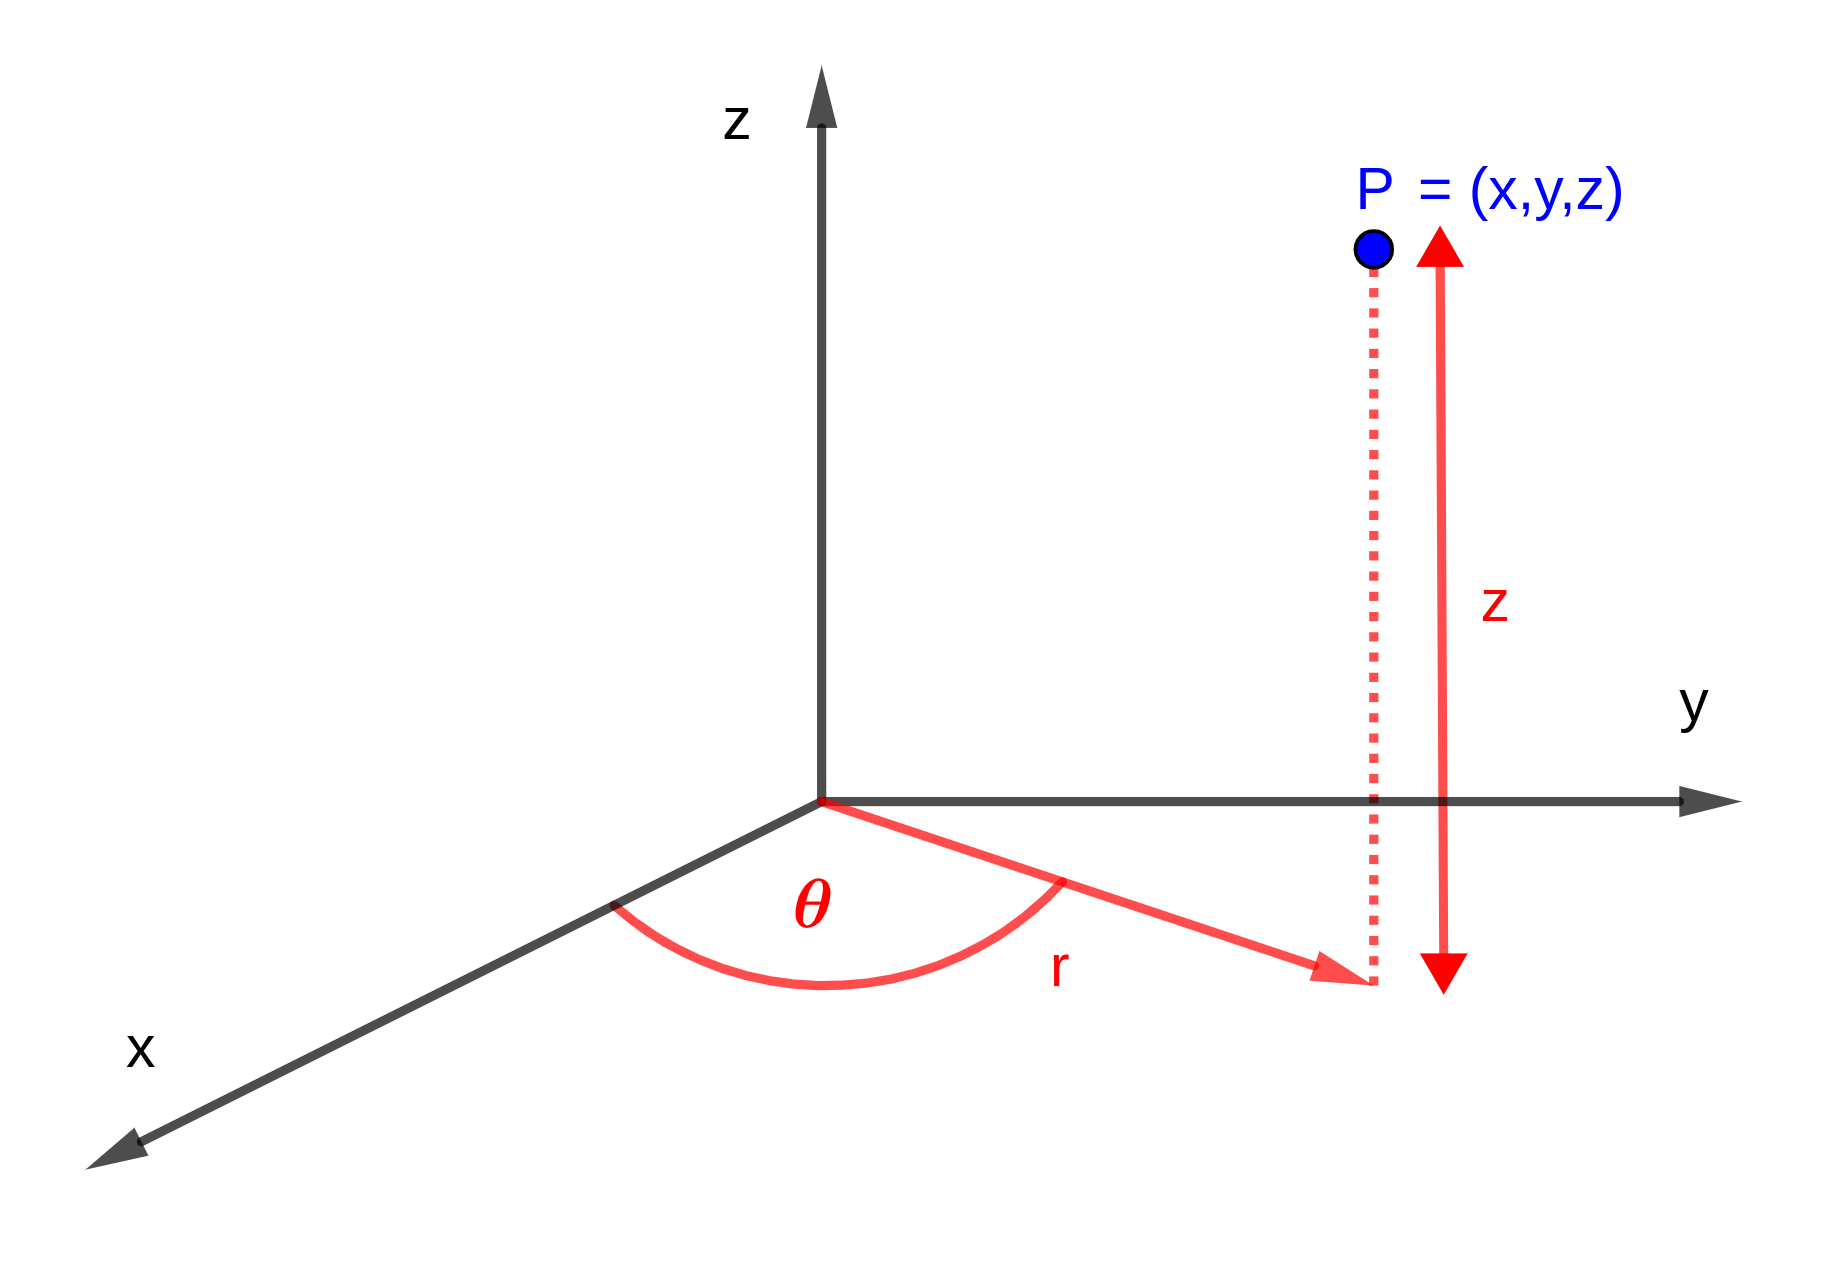
\includegraphics[scale=0.8]{img/teo_fig024_ccil.png}
\label{fig:ccil}
\end{figure}

La transformación de cilíndricas a cartesianas es $T(r, \theta, z) = (r \cos(\theta), r \sin(\theta), z)$, y su factor jacobiano es $r$.

\subsection{Coordenadas esféricas: $(\rho, \theta, \phi)$}

Estas coordenadas son un poco menos intuitivas, pero tienen su utilidad. Para visualizarlas, considérese una esfera de radio $\rho$. Para ubicar un punto en su superficie, hacen falta el ángulo respecto al eje $x$ ($\theta$) y el ángulo respecto al eje $z$ ($\phi$).

\begin{figure}[ht]
\centering
\caption{Coordenadas esféricas}
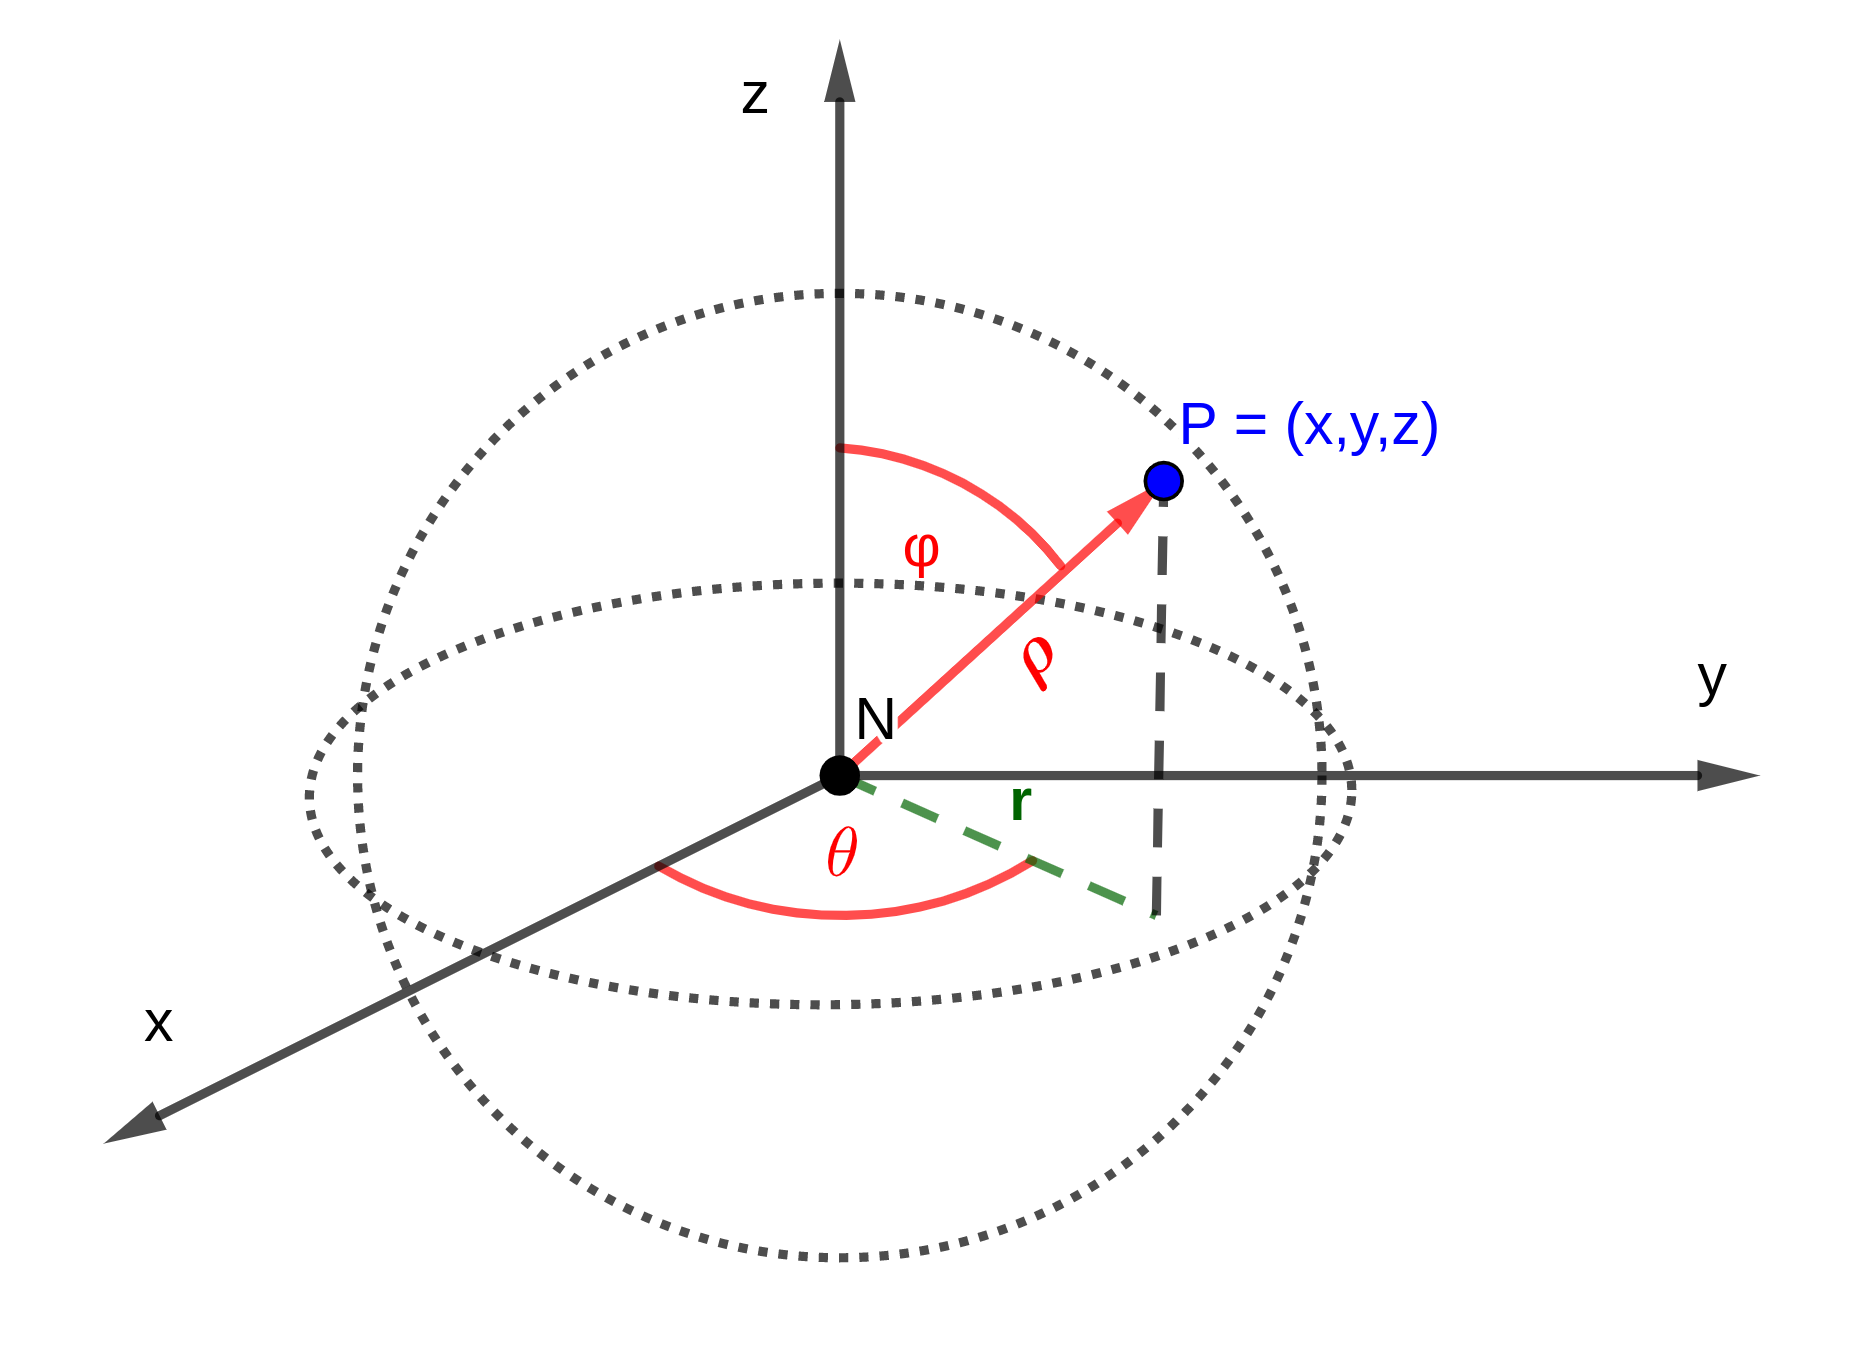
\includegraphics[scale=0.8]{img/teo_fig025_cesf.png}
\label{fig:cesf}
\end{figure}

Observando la figura~\ref{fig:cesf}, una forma práctica de conceptualizar las coordenadas esféricas de un punto $P$ en $\Bbb R^3$ es mediante los siguientes pasos:

\begin{enumerate}
\item Dibujar una esfera de radio $\rho$ igual a la norma del vector del origen al punto $P$. El punto estará sobre la superficie de la esfera.
\item Observando a $P$ desde el origen, medir el ángulo $\theta$ respecto al eje x alineado con $P$.
\item Observando a $P$ desde el origen, medir el ángulo $\phi$ respecto al eje z alineado con $P$.
\end{enumerate}

La transformación de esféricas a cartesianas es:

\begin{equation}
T(\rho, \theta, \phi) = (\rho \sin(\phi) \cos(\theta), \rho \sin(\phi) \sin(\theta), \rho \cos(\phi))
\end{equation}

El factor jacobiano es $\rho^2 \sin(\phi)$. Se verifica además:

\begin{align}
r = \rho \sin(\phi) \\
x^2 + y^2 + z^2 = \rho^2 \\
\rho^2 = r^2 + z^2
\end{align}

\subsection{Masa, centro de masa y momentos de inercia}

Dado un sólido $K$ en $\Bbb R^3$, si $\rho(x,y,z)$ es un campo escalar que describe la densidad punto a punto, resulta:

\begin{itemize}
\item $M$: masa del sólido.
\item $(\overline{x}, \overline{y}, \overline{z})$: Coordenadas del centro de masa.
\item $I_x, I_y, I_z$: Momentos de inercia.
\end{itemize}

\begin{align}
M = \iiint_K \rho(x,y,z) \mathop{dx} \mathop{dy} \mathop{dz} \\
\overline{x} = \frac{ \iiint_K x \rho(x,y,z) \mathop{dx} \mathop{dy} \mathop{dz} }{M} \\
\overline{y} = \frac{ \iiint_K y \rho(x,y,z) \mathop{dx} \mathop{dy} \mathop{dz} }{M} \\
\overline{z} = \frac{ \iiint_K z \rho(x,y,z) \mathop{dx} \mathop{dy} \mathop{dz} }{M} \\
I_x = \iiint_K (y^2 + z^2) \rho(x,y,z) \mathop{dx} \mathop{dy} \mathop{dz} \\
I_y = \iiint_K (x^2 + z^2) \rho(x,y,z) \mathop{dx} \mathop{dy} \mathop{dz} \\
I_z = \iiint_K (x^2 + y^2) \rho(x,y,z) \mathop{dx} \mathop{dy} \mathop{dz}
\end{align}

\section{Clase T17}

\subsection{Área de una superficie en $\Bbb R^3$}

Así como una curva puede parametrizarse con una variable, una superficie requiere dos variables. Ejemplos:

\begin{align}
& x^2 + y^2 = z \Rightarrow \overline{T}(u,v) = (u, v, u^2 + v^2) \\
& x^2 + y^2 + z^2 = R^2 \Rightarrow \overline{T}(\theta, \phi) = (R \sin(\phi) \cos(\theta), R \sin(\phi) \sin(\theta), R \cos(\phi)) \label{eq:supesf} \\
& \frac{x^2}{a^2} + \frac{y^2}{b^2} - \frac{z^2}{c^2} = 0 \Rightarrow \overline{T}(\theta, \phi) = (a \phi \cos(\theta), b \phi \sin(\theta), c \phi) \label{eq:supcon}
\end{align}

Nótese que las ecuaciones~\ref{eq:supesf} y~\ref{eq:supcon} están expresadas en coordenadas polares (de hecho, es bastante incómodo usar las cartesianas para dichos casos).

Sea $\overline{T}$ un campo vectorial en un conjunto abierto que contiene a $D$. $\overline{T}$ debe ser biyectivo en todo $D$, con la posible excepción de su frontera. Sean los vectores $\overline{T_u} = \frac{\partial \overline{T}}{\partial u}$ y $\overline{T_v} = \frac{\partial \overline{T}}{\partial v}$. Supóngase que dichos vectores son l.i. Si se cumplen todas estas condiciones, la superfice $S = Img(\overline{T})$ es \textbf{suave}. Puede ocurrir que la independencia lineal de $\overline{T_u}$ y $\overline{T_v}$ no se cumpla en subconjuntos de contenido nulo, y el resultado sigue valiendo.

Una forma práctica de exigir que dos vectores sean l.i. es plantear que su producto vectorial sea no nulo: $\overline{T_u} \times \overline{T_v} \neq \overline{0}$.

Entonces, para $S$ suave como en la figura~\ref{fig:asuf}, se define:

\begin{figure}[ht]
\centering
\caption{Área de una superficie}
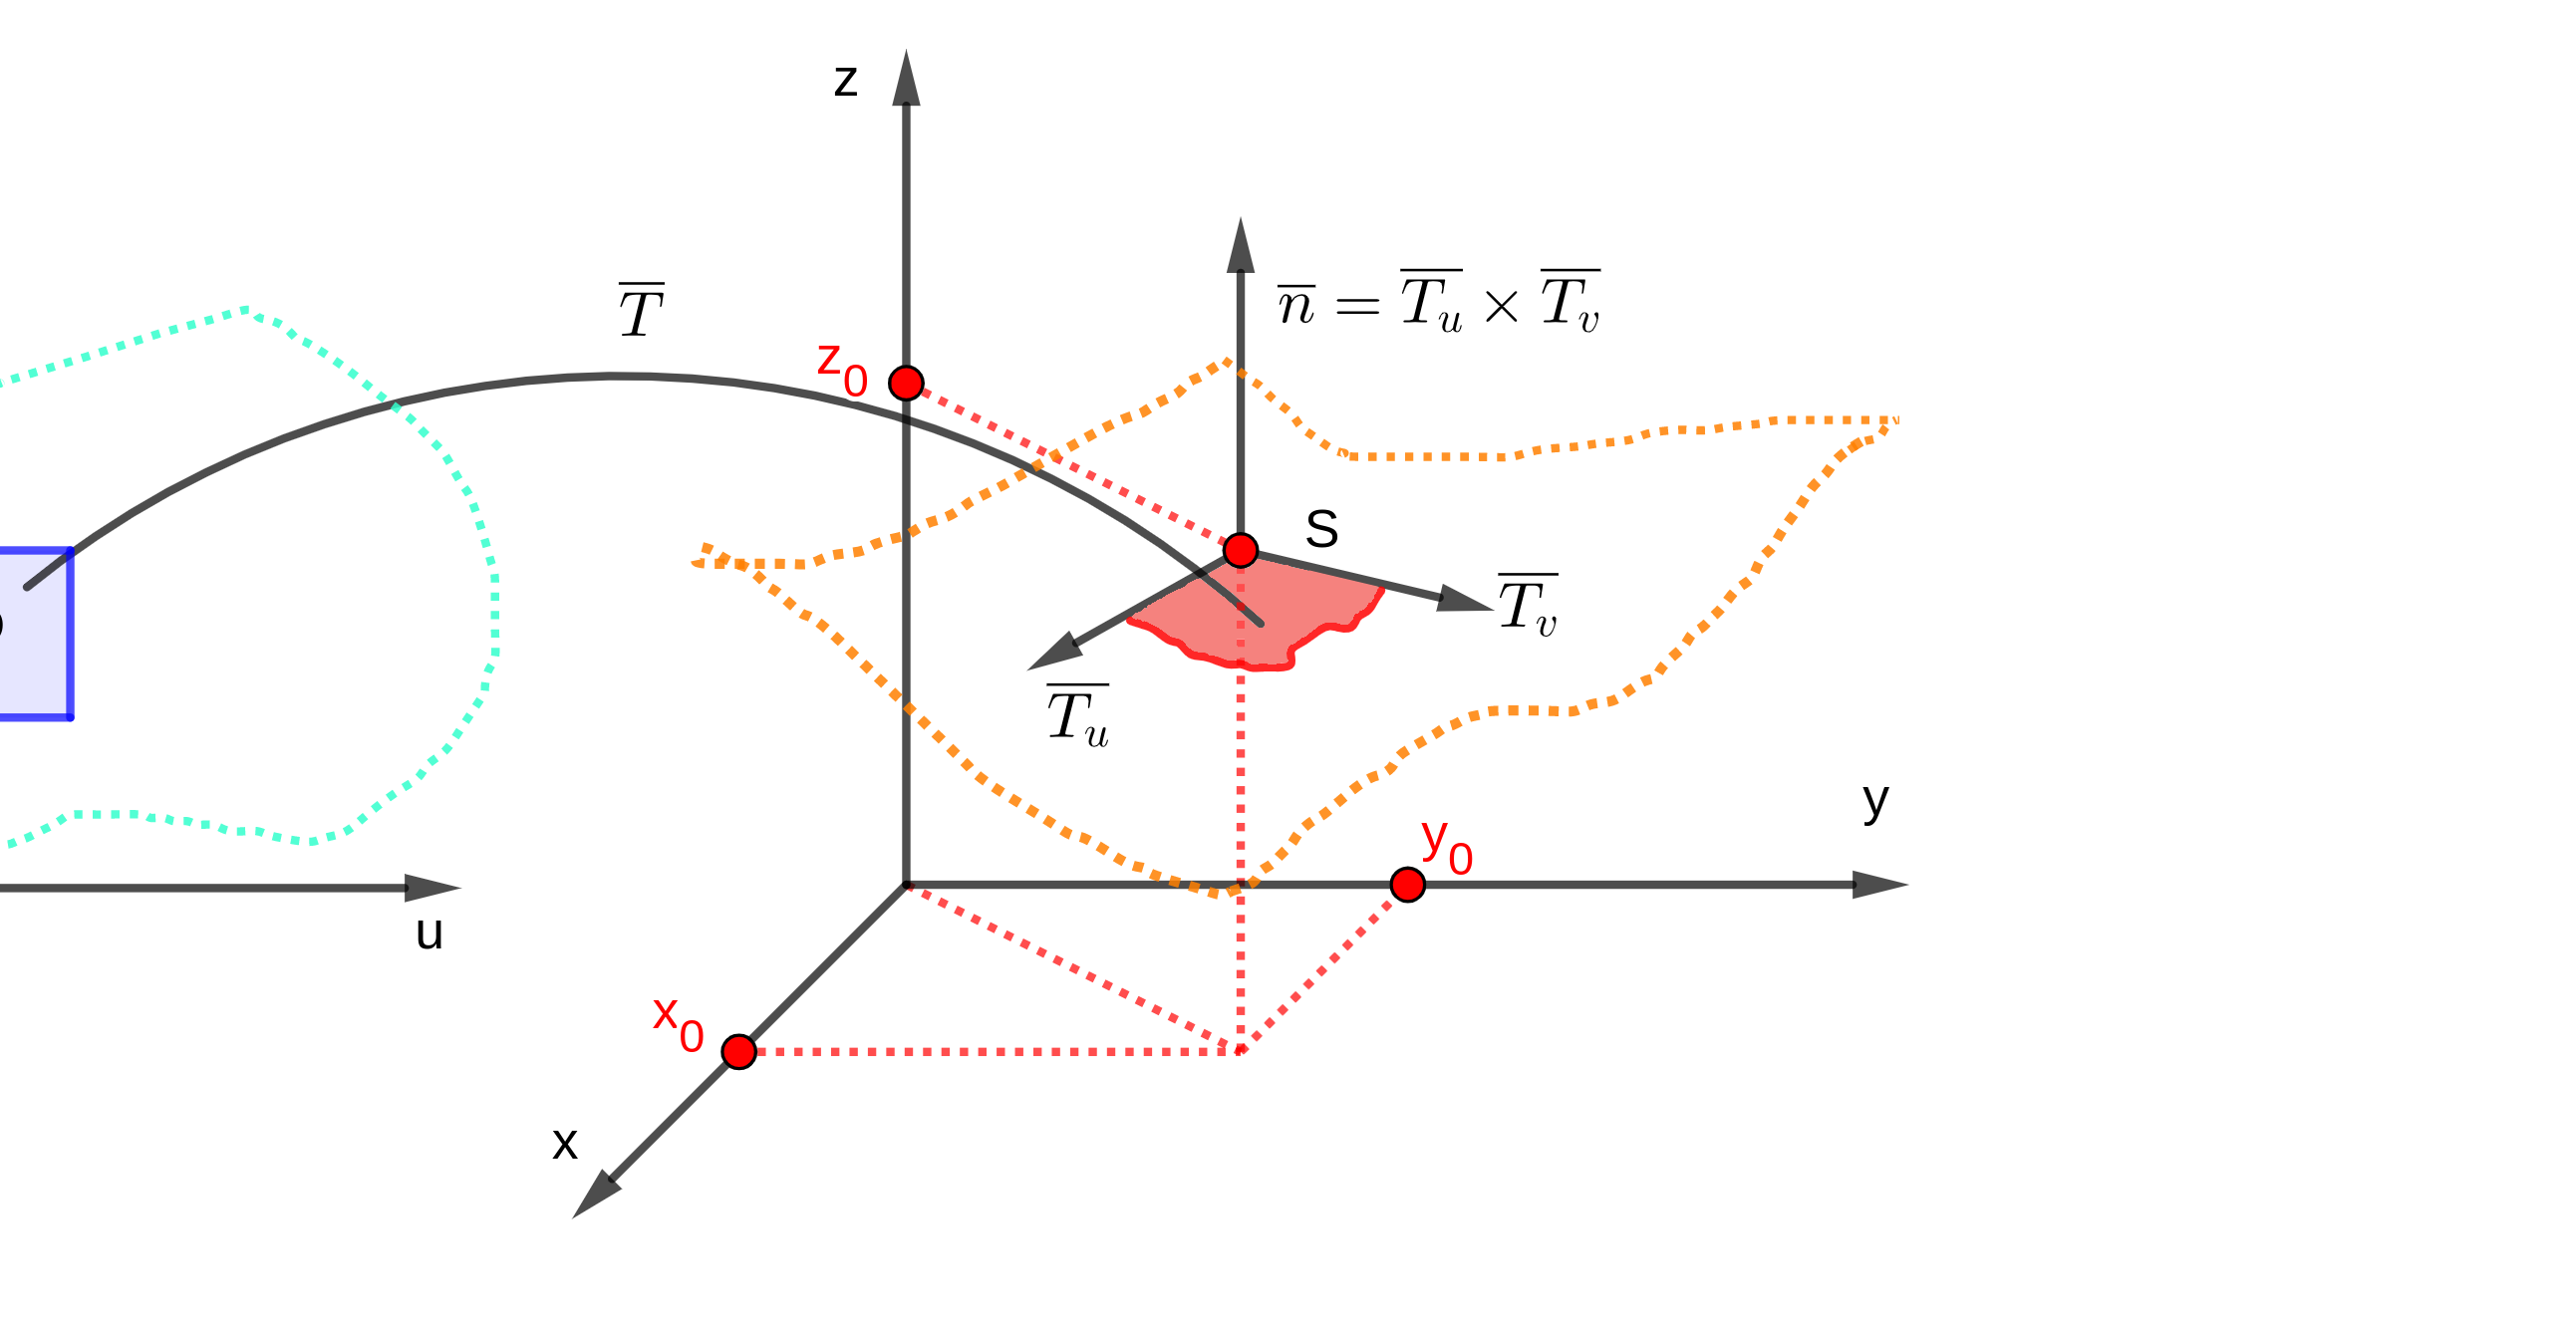
\includegraphics[scale=0.8]{img/teo_fig026_asuf.png}
\label{fig:asuf}
\end{figure}

\begin{equation}
\tcboxmath[colback=orange!25!white,colframe=orange, title=Área de una superficie]
{ \mathop{area}(S) = \iint_S dS, \text{ con } dS = \underbrace{ \left|\left| \overline{T_u} \times \overline{T_v} \right|\right| }_{J_{\overline{T}}} \mathop{du} \mathop{dv} }
\end{equation}

\subsection{Integral de un CE sobre una superficie}

Dadas una superficie $S$ suave en $\Bbb R^3$, y un campo escalar $f:\Bbb R^3 \rightarrow \Bbb R$ continuo sobre un conjunto abierto que contiene a $S$:

\begin{equation}
\tcboxmath[colback=orange!25!white,colframe=orange, title=Integral de un CE sobre una superficie]
{ \iint_S f \mathop{dS} = \iint_{D_{uv}} f(T(u,v)) \left|\left| \overline{T_u} \times \overline{T_v} \right|\right| \mathop{du} \mathop{dv} }
\end{equation}

En esta notación, $D_{uv}$ se refiere a los límites superiores e inferiores de los parámetros $u$ y $v$ que definen la superficie $S$ en su versión parametrizada $T(u,v)$.

\subsection{Integral de un CV sobre una superficie}

Con las mismas condiciones que para un CE, dado $\overrightarrow{f}:\Bbb R^3 \rightarrow \Bbb R$ continuo en un abierto que contiene a $S$, se define:

\begin{equation}
\tcboxmath[colback=orange!25!white,colframe=orange, title=Integral de un CV sobre una superficie: flujo]
{ \iint_S \overrightarrow{f} \cdot \mathop{\overrightarrow{dS}} = \iint_{D_{uv}} \overrightarrow{f}(T(u,v)) \underbrace{\cdot}_{\text{prod. escalar}} \underbrace{ \left( \overline{T_u} \times \overline{T_v} \right) \mathop{du} \mathop{dv}}_{\mathop{\overrightarrow{dS}}} }
\end{equation}

Este tipo de integral suele denominarse el \textbf{flujo} del campo vectorial $f$ sobre la superficie $S$.

\subsection{Expresión del área para una superficie definida en forma implícita}

Sea $F(x,y,z) = 0$. Dadas las condiciones del TFI, existe $z = f(x,y)$, y además $z_x = -\frac{F_x}{F_z} \wedge z_y = -\frac{F_y}{F_z}$. Si $S$ es la superficie asociada a $z = f(x,y)$, puede probarse que, dadas las condiciones:

\begin{equation}
\mathop{area}(S) = \iint_{R} \frac{ || \overrightarrow{\nabla F}|| }{ | \overrightarrow{ \nabla F } \cdot \overrightarrow{n} | } \mathop{dA}
\end{equation}

En esta expresión, $R$ es la proyección de la superficie $S$ sobre un plano elegido convenientemente. El vector $\overrightarrow{n}$ es el versor $\hat{i}, \hat{j}$ o $\hat{k}$ que sea normal a $R$ y cumpla $\overrightarrow{ \nabla F } \cdot \overrightarrow{n} \neq 0$. Por ejemplo, si $R$ está en el plano $xy$, $\overrightarrow{p} = \hat{k}$, porque $\hat{k}$ está asociado al eje $z$, que es normal al plano $xy$. En cuanto a $dA$, será $\mathop{du} \mathop{dv}$ para coordenadas cartesianas, y $r \mathop{dr} \mathop{d\theta}$ para coordenadas polares. Para visualizar la relación entre $S$ y $R$, obsérvese la figura~\ref{fig:isi}.

\begin{figure}[ht]
\centering
\caption{La superficie S y su proyección R}
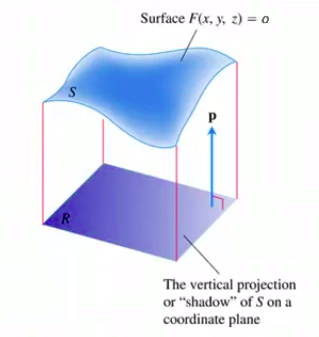
\includegraphics[scale=0.8]{img/teo_fig027_isi.png}
\label{fig:isi}
\end{figure}

Por ejemplo, dada la esfera de radio 2, con ecuación implícita $x^2 + y^2 + z^2 = 2$, se desea calcular el área de la superficie superior delimitada al cortarla con el plano $z = 1$. Un gráfico de dicha superficie puede apreciarse en la figura~\ref{fig:isiej}

\begin{figure}[ht]
\centering
\caption{Superficie S}
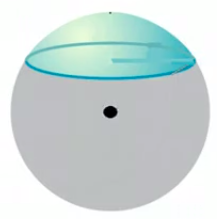
\includegraphics[scale=0.8]{img/teo_fig028_isi.png}
\label{fig:isiej}
\end{figure}

En este caso:

\begin{align}
F(x,y,z) &= x^2 + y^2 + z^2 - 2 \\
\overrightarrow{\nabla F}(x,y,z) &= (2x, 2y, 2z) \\
||\overrightarrow{\nabla F}(x,y,z)|| &= \sqrt{4x^2 + 4y^2 + 4z^2} = \sqrt{4 \underbrace{(x^2 + y^2 + z^2)}_{2}} = 2 \sqrt{2}
\end{align}

Para calcular la proyección $R$, considérese que es la intersección entre $x^2 + y^2 + z^2 = 2$ y $z = 1$. Reemplazando $z = 1$ en la ecuación de la esfera, resulta $x^2 + y^2 = 1$, que es un círculo en el plano $xy$. Esto ya establece que $\overrightarrow{n} = \hat{k} \Rightarrow | \overrightarrow{ \nabla F } \cdot \hat{k}| = |2z| = 2z$. El módulo se elimina porque en el intervalo de interés, $z$ es siempre positivo. Entonces:

\begin{equation}
\mathop{area}(S) = \iint_R \frac{2 \sqrt{2}}{2z} \mathop{dA} = \sqrt{2} \iint_R \frac{1}{z} dA 
\end{equation}

$R$ es un círculo, por lo cual lo más sensato es utilizar coordenadas polares. Por lo tanto, tener $z$ en el integrando no sirve. Despejando $z$ en la ecuación de la esfera, resulta:

\begin{equation}
z = \sqrt{2 - \underbrace{ (x^2 + y^2) }_{r^2}} = \sqrt{2 - r^2}
\end{equation}

Dado que se usan coordenadas polares, $dA = r \mathop{dr} \mathop{d\theta}$. Dado que $R$ es un círculo unidad, $r$ va de $0$ a $1$, y $\theta$ va de $0$ a $2\pi$. Ergo:

\begin{equation}
\mathop{area}(S) = \sqrt{2} \int_0^{2\pi} \int_0^1 \frac{1}{\sqrt{2 - r^2}} r \mathop{dr} \mathop{d\theta}
\end{equation}

Con la sustitución $u = 2 - r^2$, se simplifica la integral y resulta $\mathop{area}(S) = 2\pi (2 - \sqrt(2)) \approx 3.68$

\subsection{Superficie orientable}

Una superficie es orientable $\Leftrightarrow$ tiene sólo dos normales posibles en cada punto. Se dice que en una superficie de ese tipo se ha definido una orientación si se ha adoptado un campo de normales dado por $( \overrightarrow{T_u} \times \overrightarrow{T_v} )$

En el caso particular de superficies cerradas (como una esfera), se define la orientación positiva como aquella donde las normales apuntan hacia la región no acotada, o externa, de la superficie. Por descarte, la otra orientación es la negativa. Por ejemplo, en la figura~\ref{fig:son}, la normal positiva es la negra, y la negativa es la roja.

\begin{figure}[ht]
\centering
\caption{Orientación positiva y negativa}
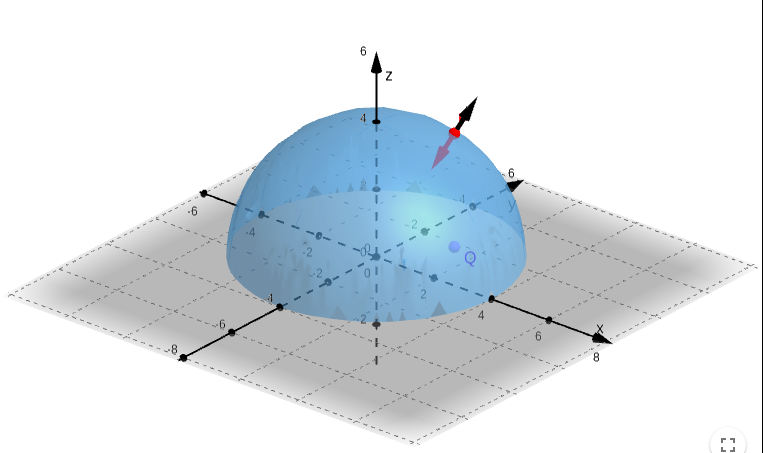
\includegraphics[scale=0.6]{img/teo_fig029_son.png}
\label{fig:son}
\end{figure}

\subsection{Divergencia y rotor}

Dado un CV $C^1$, $\overline{f}: \Bbb R^n \rightarrow \Bbb R^n$, se define su \textbf{divergencia} como:

\begin{equation}
\tcboxmath[colback=orange!25!white,colframe=orange, title=Divergencia de un CV]
{ \mathop{div} \overline{f} = \frac{\partial f_1}{x_1} + \frac{\partial f_2}{x_2} + \ldots + \frac{\partial f_n}{x_n} }
\end{equation}

Nótese que es un CE de $n$ variables.

Sólo para el caso de $\Bbb R^3$, se define el \textbf{rotor} como:

\begin{align}
&\overline{f}:\Bbb R^3 \rightarrow \Bbb R^3 / \overline{f}(x,y,z) = (f_1(x,y,z), f_2(x,y,z), f_3(x,y,z)) \\
&\mathop{\overline{rot}} \overline{f} = \left( \frac{\partial f_3}{\partial y} - \frac{\partial f_2}{\partial z}, \frac{\partial f_1}{\partial z} - \frac{\partial f_3}{\partial x}, \frac{\partial f_2}{\partial x} - \frac{\partial f_1}{\partial y}  \right)
\end{align}

Una forma simbólica de recordar esta definición es, mediante un abuso de notación, asociarla a un producto vectorial:

\begin{equation}
\mathop{\overline{rot}} \overline{f} = \overrightarrow{\nabla} \times \overline{f} = \begin{vmatrix}
\hat{i} & \hat{j} & \hat{k} \\
\frac{\partial}{\partial x} & \frac{\partial}{\partial y} & \frac{\partial}{\partial z} \\
f_1 & f_2 & f_3
\end{vmatrix}
\end{equation}

El rotor del gradiente de un CE $C^2$, por Schwartz, es nulo.

Los CV de rotor nulo se llaman \textbf{irrotacionales}. Un campo de gradientes, para el cual existe $\Phi$, es siempre irrotacional.

\subsection{Laplaciano}

Sea $f$ un CE $C^2$. Se define entonces el laplaciano de $f$ como la suma de las derivadas parciales segundas repetidas:

\begin{equation}
\nabla^2 f = f_{x_1 x_1} + f_{x_2 x_2} + \ldots + f_{x_n x_n}
\end{equation}

Los CE con laplaciano nulo se denominan \textbf{armónicos}.

\subsection{Teorema de Green}

\begin{figure}[ht]
\centering
\caption{Teorema de Green}
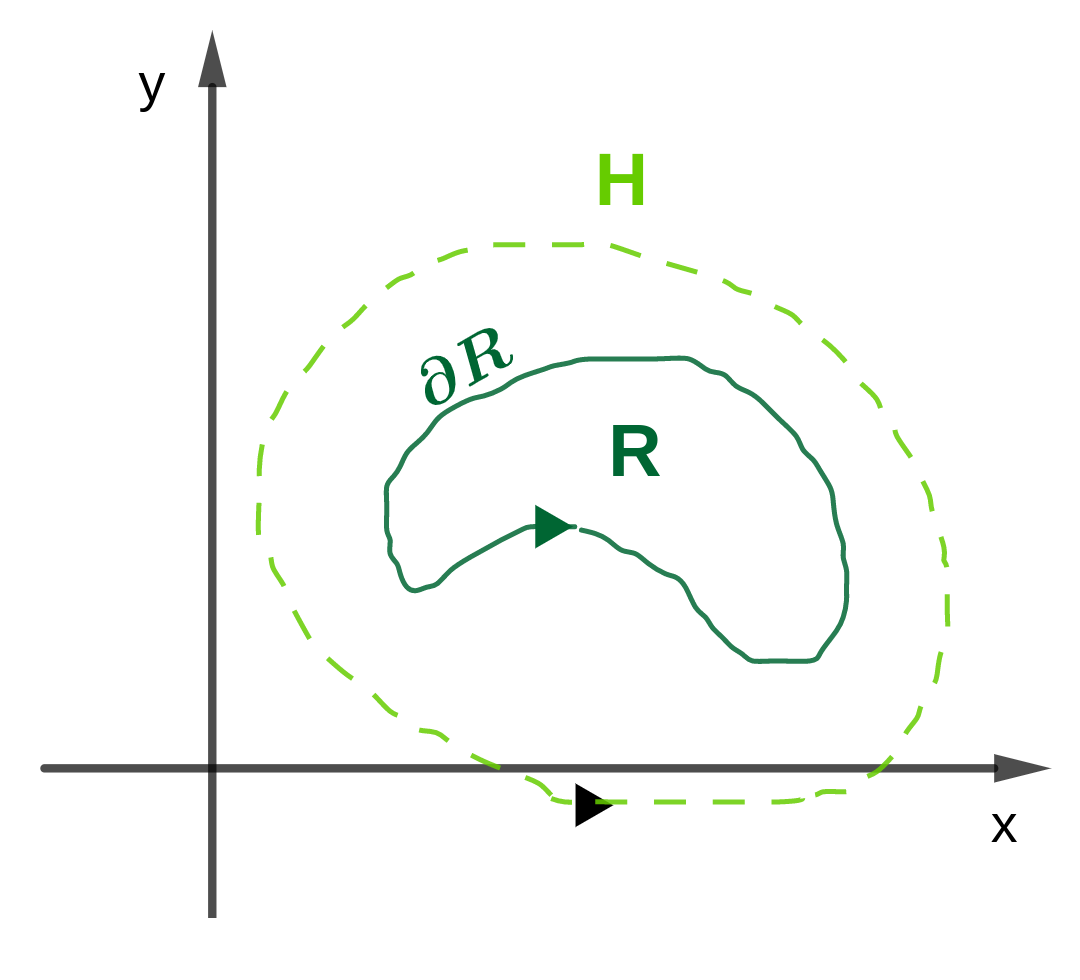
\includegraphics[scale=0.85]{img/teo_fig030_green.png}
\label{fig:green}
\end{figure}

Obsérvese la figura~\ref{fig:green}. En el contexto de la misma, sean:

\begin{align}
& \overline{f}:H \subset \Bbb R^2 \rightarrow \Bbb R^2 / f(x,y) = (P(x,y), Q(x,y)) \\
& \partial^+ R = C \text{ (la frontera de } R \text{ es una curva)}
\end{align}

Si el CV $\overline{f}$ es $C^1$ en un conjunto abierto $H \subset \Bbb R^2$ que contiene a un lazo simple $\partial^+ R$ $C^1$ y con derivadas primeras no nulas, entonces:

\begin{equation}
\tcboxmath[colback=orange!25!white,colframe=orange, title=Teorema de Green]
{ \ointctrclockwise_{\partial^+ R} \overline{f} \cdot \mathop{d(\partial^+R)} = \iint_R [Q_x(x,y) - P_y(x,y)] \mathop{dx} \mathop{dy} }
\end{equation}

\section{Clase T18}

\subsection{Observaciones sobre el teorema de Green}

\begin{enumerate}
\item El teorema es igualmente válido cuando el lazo $R$ es construido mediante la unión de varias curvas suaves.

\item Dadas las condiciones del teorema, con $H$ simplemente conexo, las siguientes afirmaciones son equivalentes entre sí:
\begin{enumerate}
\item $\exists \Phi / \overline{f} = \nabla \Phi$, o sea que $\overline{f}$ es un CG.
\item $\forall P \in H, P_y(P) = Q_x(P)$
\item La integral curvilínea de $\overline{f}$ entre dos puntos dentro de $H$ no depende de la trayectoria, y la integral curvilínea sobre el lazo $R$ es nula. Esto se demuestra justamente con el teorema de Green.
\end{enumerate}

\item Sea $\overline{f} = (P(x,y), Q(x,y))$ con $P_y = Q_x$ en el conjunto $H$, y sean las curvas $C_1, C_2 y C_3$ como se ven en la figura~\ref{fig:green31}.

\begin{figure}[ht]
\centering
\caption{Green en región conexa}
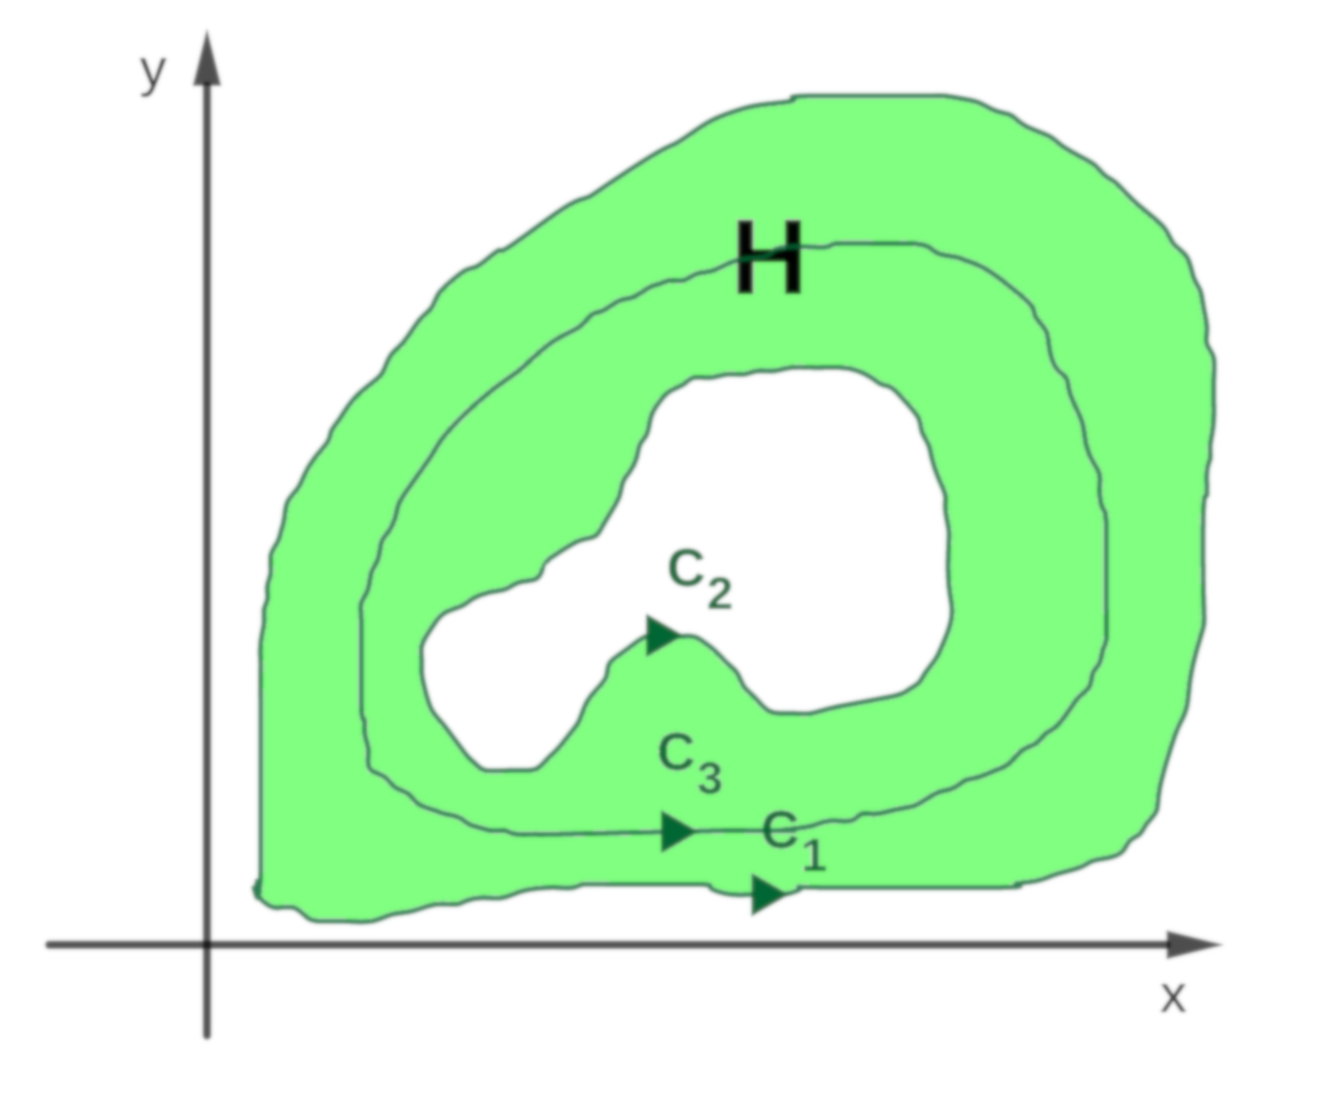
\includegraphics[scale=0.85]{img/teo_fig031_green.png}
\label{fig:green31}
\end{figure}

Dado que $C_1$ y $C_2$ están en la frontera de $H$, no se puede asegurar que la integral sobre ellas sea cero. Sin embargo, el teorema de Green garantiza la siguiente igualdad:

\begin{equation}
\int_{C_1^+} \overline{f} \cdot \mathop{\overline{dC_1}} = \int_{C_2^+} \overline{f} \cdot \mathop{\overline{dC_2}} = \int_{C_3^+} \overline{f} \cdot \mathop{\overline{dC_3}}
\end{equation}

Esbozo de demostración: considérese la curva $\gamma_1$, que conecta $C_1$ y $C_2$ en la figura~\ref{fig:green32}.

\begin{figure}[ht]
\centering
\caption{Green en región conexa}
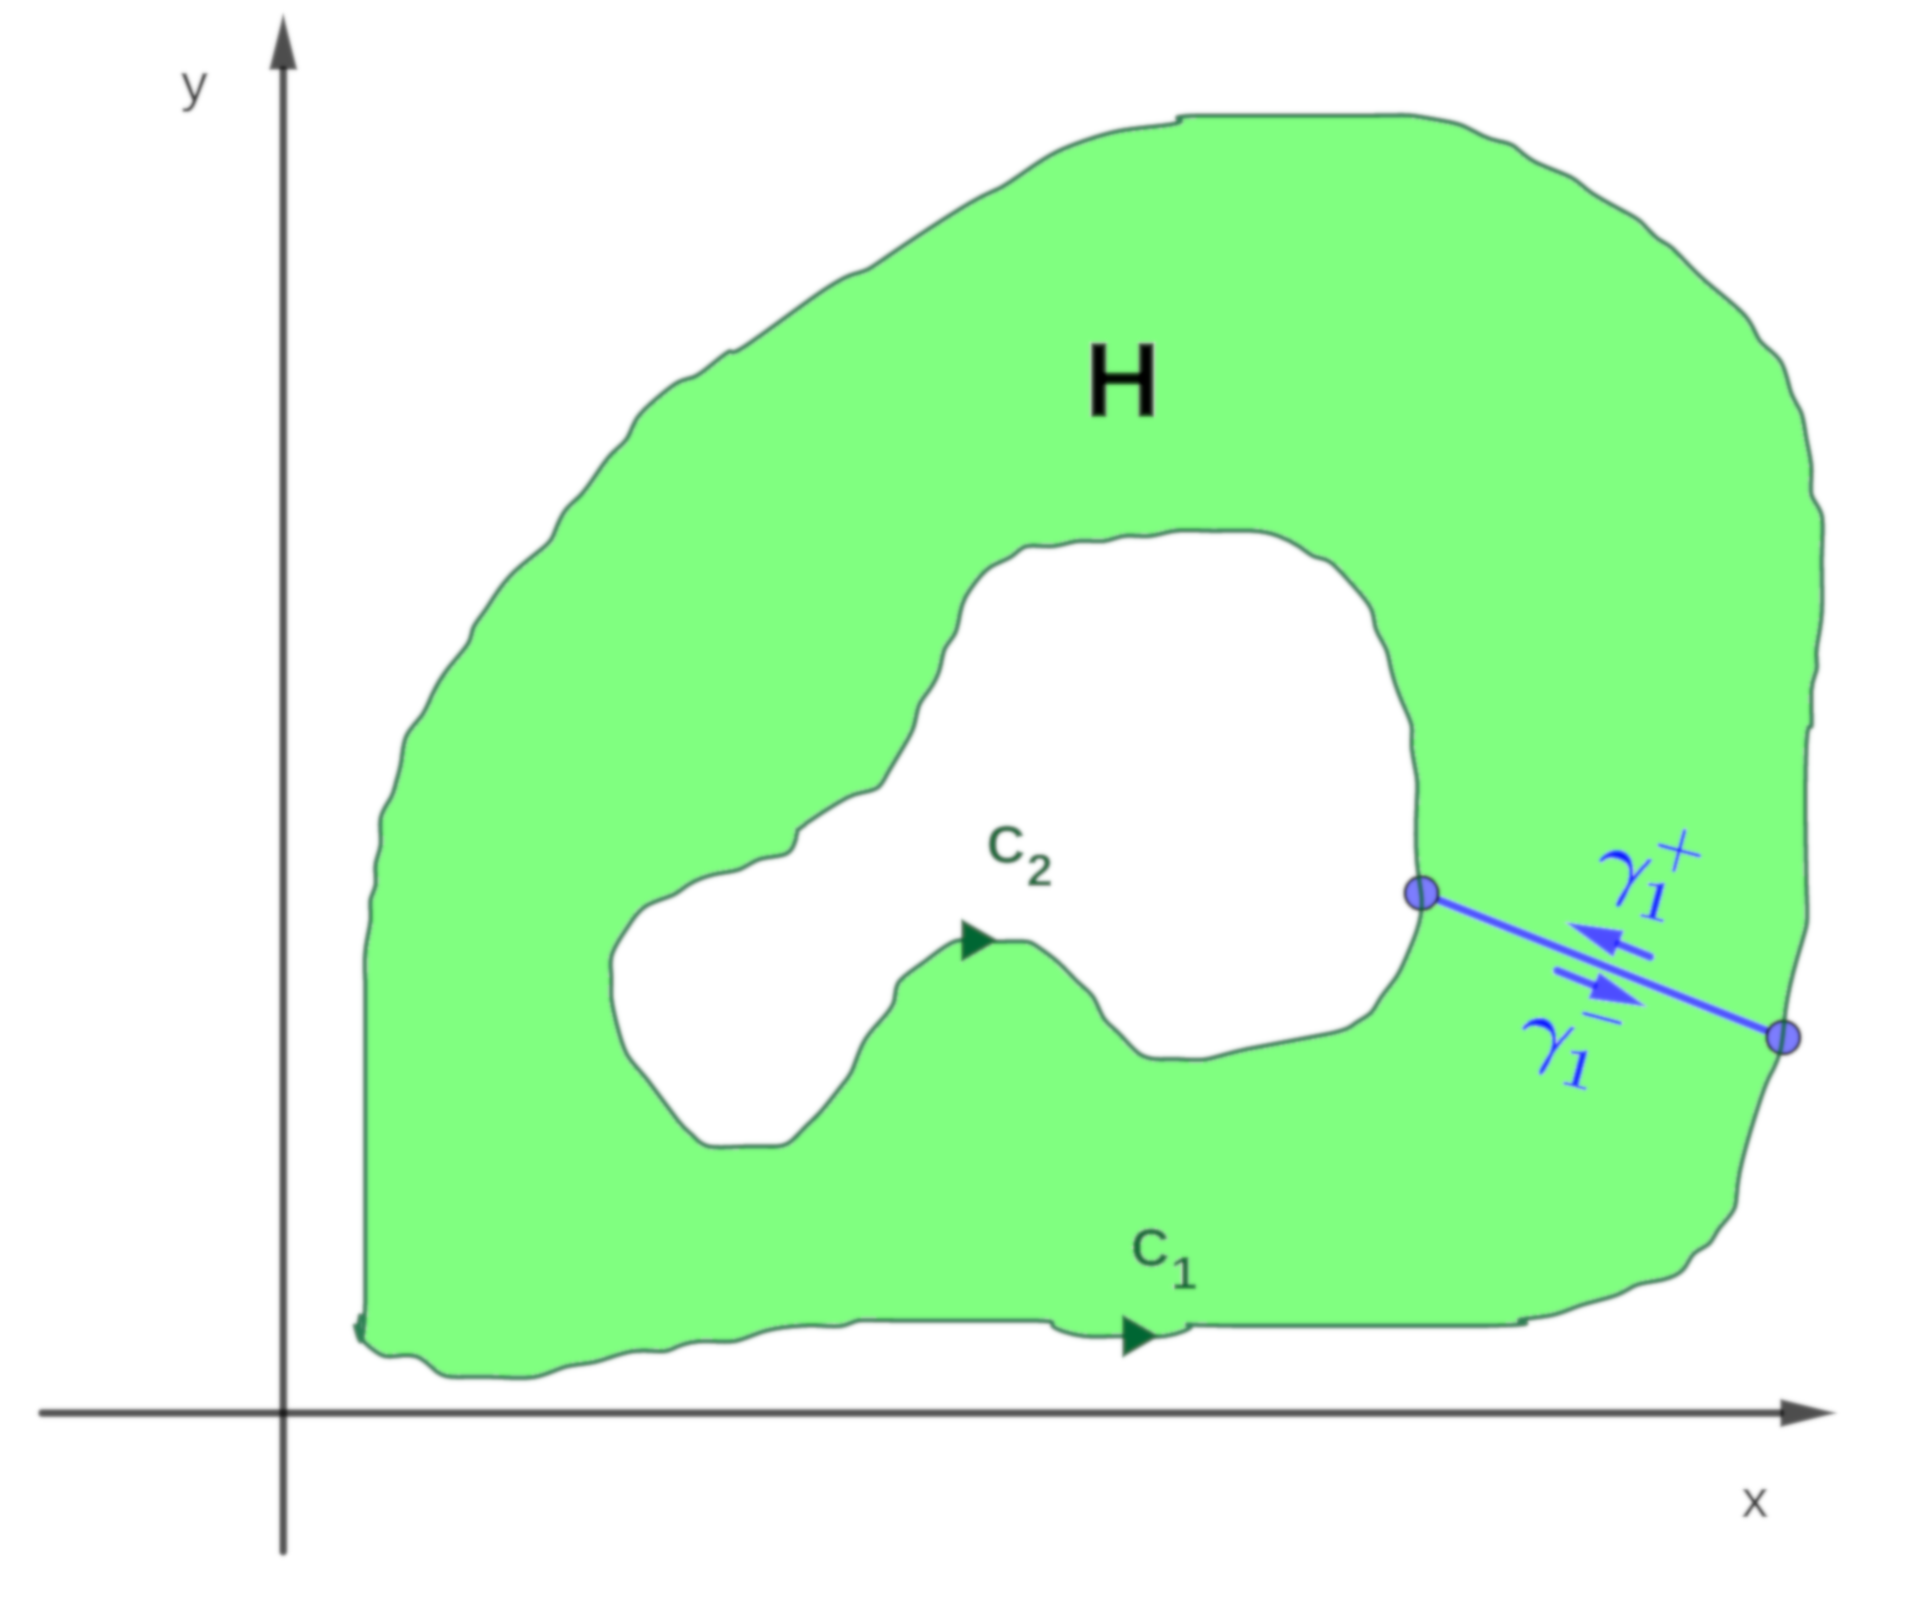
\includegraphics[scale=1]{img/teo_fig032_green.png}
\label{fig:green32}
\end{figure}

Sea entonces $\sigma = C_1^+ \cup \gamma_1^+ \cup C_2^- \cup \gamma_1^-$, donde los sentidos positivos de $C_1$ y $C_2$ son los de la figura ~\ref{fig:green32}, y los sentidos de $\gamma_1$ son los de la figura ~\ref{fig:green32}. Por lo tanto:

\begin{equation}
\ointctrclockwise_{\sigma} \overline{f} \cdot \mathop{\overline{d\sigma}} = \int_{C_1^+} \overline{f} \cdot \mathop{\overline{dC_1}} + \bcancel{ \int_{\gamma_1^+} \overline{f} \cdot \mathop{\overline{d\gamma_1}} } + \int_{C_2^-} \overline{f} \cdot \mathop{\overline{dC_2}} + \bcancel{ \int_{\gamma_1^-} \overline{f} \cdot \mathop{\overline{d\gamma_1}} }
\end{equation}

Las integrales sobre $\gamma_1$ se cancelan por ser el mismo recorrido con sentido opuesto, con $f \in C^1$ y $\gamma_1$ suave. Por Green, $\sigma$ es un lazo donde vale la simetría de las derivadas y el interior de $\sigma$ está contenido en $H$, por lo tanto:

\begin{equation}
\ointctrclockwise_{\sigma} \overline{f} \cdot \mathop{\overline{d\sigma}} = 0 \Rightarrow 0 = \int_{C_1^+} \overline{f} \cdot \mathop{\overline{dC_1}} + \int_{C_2^-} \overline{f} \cdot \mathop{\overline{dC_2}} \Rightarrow \int_{C_1^+} \overline{f} \cdot \mathop{\overline{dC_1}} = \int_{C_2^+} \overline{f} \cdot \mathop{\overline{dC_2}}
\end{equation}

La igualdad con $C_3$ puede probarse de forma similar.

\item Cualquier CV que satisfaga $-P_y + Q_x = k$ sirve para calcular áreas de regiones planas. En particular, son de utilidad los CVs $\overline{f} = (0, x)$, $\overline{f} = (-y, 0)$ y $\overline{f} = (-y, x)$.

\end{enumerate}

\section{Clase T19}

\subsection{Teorema de Stokes}

Este teorema es una extensión del teorema de Green, pasando de 2 a 3 dimensiones.

\begin{figure}[ht]
\centering
\caption{Teorema de Stokes}
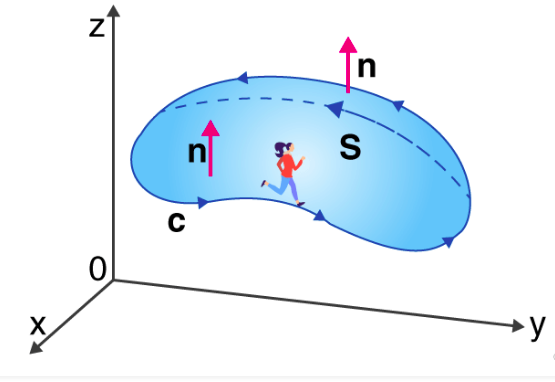
\includegraphics[scale=0.5]{img/teo_fig033_stokes.png}
\label{fig:stokes}
\end{figure}

Como se observa en la figura~\ref{fig:stokes}, se tiene una curva cerrada tridimensional $C \in C^1$ en la región de interés. Dicha curva es, geométricamente la base de una superficie $S$, cuya parametrización en dos variables, $T(u,v) \in C^1$ en la región de interés. Además, el sentido de circulación de la curva  es positivo: si se imagina una persona caminando sobre la curva, su cabeza apuntará en el sentido en que la superficie "emerge" de la curva, como se observa en la figura ~\ref{fig:stokes}.

Dadas todas estas condiciones, el teorema de Stokes garantiza que, para un campo vectorial $\overline{f}: A \subset \Bbb R^3 \rightarrow \Bbb R^3 \in C^1(A)$:

\begin{equation}
\tcboxmath[colback=orange!25!white,colframe=orange, title=Teorema de Stokes]
{ \ointctrclockwise_C \overline{f} \cdot \mathop{\overline{dC}} = \iint_S \mathop{rot}\overline{f} \cdot \mathop{\overline{dS}}
 }
\label{eq:stokes}
\end{equation}

En esta expresión, $\mathop{\overline{dS}} = \hat{n} \mathop{dS}$, siendo $\hat{n}$ un vector de norma 1 en la dirección normal a la superfice $S$, punto a punto.

El lado izquierdo de la igualdad en la ecuación~\ref{eq:stokes} es la circulación del campo $\overline{f}$ sobre la curva $C$. El lado derecho es el flujo del rotor de dicho campo sobre la superficie orientada $S$. Claramente, la elección de $S$ es irrelevante: esto se cumple para cualquier $S$ cuya parametrización sea $C^1$ en la región de interés. Por lo tanto, elegir $S$ inteligemente puede simplificar mucho los cálculos.

\subsubsection{Observaciones}

\begin{enumerate}
\item El flujo del rotor de un campo $C^1$ sobre una superficie cerrada y $C^1$ siempre es cero. Intuitivamente, una superficie cerrada siempre puede seccionarse en dos partes con una curva. Si dicha curva, suave, juega el rol de $C$ en el teorema de Stokes, el flujo total del rotor sobre la superficie puede calcularse como la suma del flujo en cada mitad. Como ambas mitadas tienen como base la misma curva $C$, pero con sentido de circulación opuesto, siempre se cancelarán entre sí, como se aprecia en la figura~\ref{fig:stokes2}.

\begin{figure}[ht]
\centering
\caption{Stokes sobre superficie cerrada}
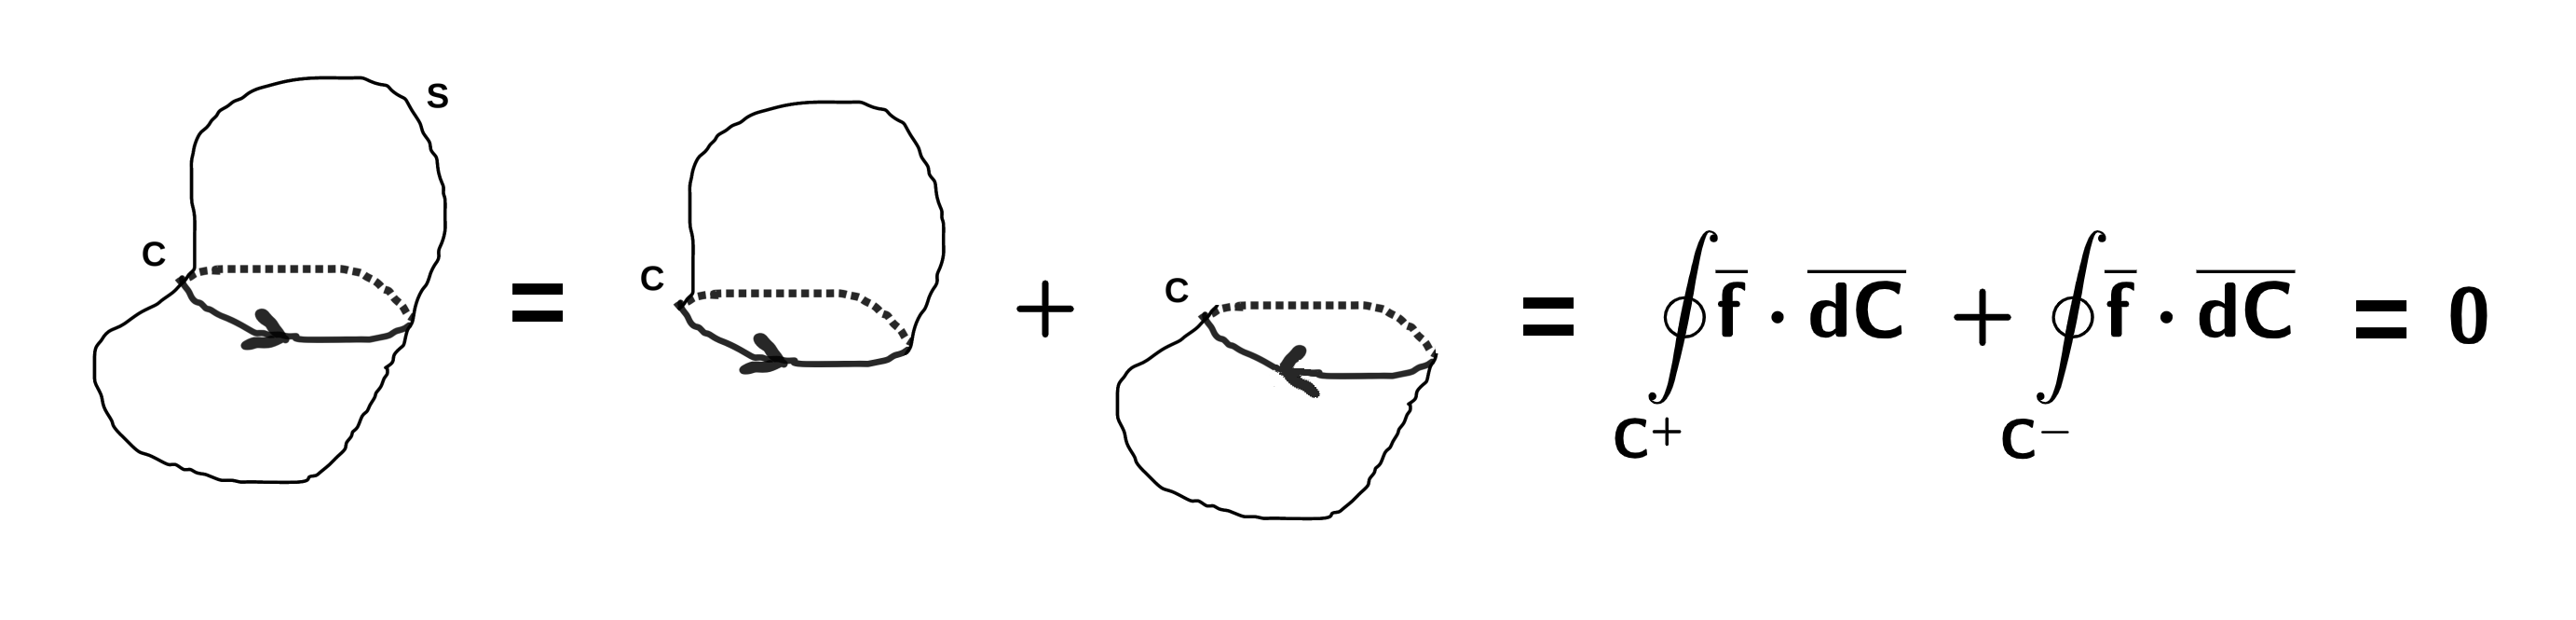
\includegraphics[scale=0.7]{img/teo_fig034_stokes.png}
\label{fig:stokes2}
\end{figure}

\item El teorema de Green es un caso particular del teorema de Stokes. Si $C$ es plana y se ubica en el plano $xy$, se elige $S$ como la superficie también plana delimitada por $C$, y se anula la componente $z$ del CV tal que $\overline{f} = (P, Q, 0)$, aplicando el teorema de Stokes se obtiene:

\begin{align}
& \ointctrclockwise_C \overline{f} \cdot \mathop{\overline{dC}} = \iint_S \mathop{rot} \overline{f} \cdot (0,0,1) \mathop{dx} \mathop{dy} = \iint_S \begin{vmatrix}
\hat{i} & \hat{j} & \hat{k} \\
\frac{\partial}{\partial x} & \frac{\partial}{\partial y} & \frac{\partial}{\partial z} \\
P & Q & 0
\end{vmatrix} \cdot (0,0,1) \mathop{dx} \mathop{dy} = \\
& \iint_S (0, 0, Q_x - P_y) \cdot (0,0,1) \mathop{dx} \mathop{dy} = \iint_S (Q_x - P_y) \mathop{dx} \mathop{dy} 
\end{align}

\item Ejemplo: se desea calcular el flujo del rotor del campo $\overline{F} = (xz, yz, xy)$ sobre la superficie $S$ definida por la parte de la esfera $x^2 + y^2 + z^2 = 4$ contenida en el cilindro $x^2 + y^2 = 1$.

Como primer paso, se grafica $S$ en la figura~\ref{fig:stokesex}.

\begin{figure}[ht]
\centering
\caption{Ejemplo Stokes}
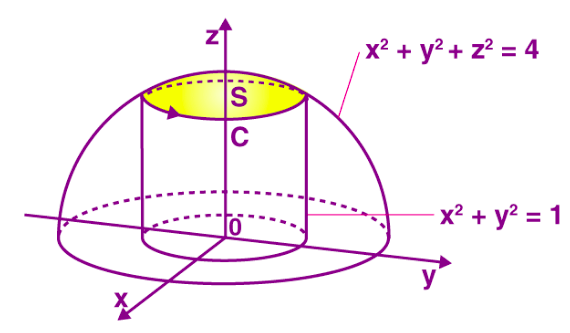
\includegraphics[scale=0.7]{img/teo_fig035_stokesex.png}
\label{fig:stokesex}
\end{figure}

La curva $C$ más conveniente es el círculo de radio 1 donde se intersectan la esfera y el círculo. Para hallar el valor de $z$ asociado, considérese las ecuaciones de ambas cónicas a la vez:

\begin{equation}
\left\{
\begin{array}{ll}
x^2 + y^2 + z^2 = 4 \\
x^2 + y^2 = 1
\end{array}
\right. \Rightarrow (1) - (2): z^2 = 3 \Rightarrow z = \sqrt{3}
\end{equation}

Ahora bien, siendo $S, \overline{F}$ y $C$ todos $C^1$, vale Stokes:

\begin{equation}
\ointctrclockwise_C \overline{F} \cdot \mathop{\overline{dC}} = \iint_S \mathop{rot}\overline{F} \cdot \mathop{\overline{dS}}
\end{equation} 

Lo más sencillo de calcular en este caso es el lado izquierdo. Recordando el cálculo de la integral de línea en base a una curva monoparamétrica:

\begin{equation}
\ointctrclockwise_C \overline{F} \cdot \mathop{\overline{dC}} = \int_a^b \overline{F}(\overline{r(t)}) \cdot r'(t) dt
\end{equation}

Para este ejemplo, $r(t)$ sería:

\begin{align}
\overline{r}(t) &= \left( \cos (t), \sin (t), \sqrt{3} \right), 0 \leq t \leq 2\pi \\
\overline{r'}(t) &= \left( -\sin (t), \cos (t), 0 \right)
\end{align}

Evaluando el CV en la curva:

\begin{equation}
\overline{F}(\overline{r(t)}) = \left( \cos(t) \sqrt(3), \sin(t) \sqrt(3), \cos(t) \sin(t) \right)
\end{equation}

Finalmente:

\begin{align}
& \iint_S \mathop{rot}\overline{F} \cdot \mathop{\overline{dS}} = \int_0^{2\pi} \left( \cos(t) \sqrt(3), \sin(t) \sqrt(3), \cos(t) \sin(t) \right) \cdot \left( -\sin (t), \cos (t), 0 \right) dt = \\
& \int_0^{2pi} \left( -\sqrt{3} \cos(t) \sin(t) + \sqrt{3} \cos(t) \sin(t) \right) dt = \sqrt{3} \int_0^{2\pi} 0 dt = 0
\end{align}

Cabía esperar este resultado por la simetría de $S$ y del campo $F$.

\end{enumerate}

\end{document}